% !TeX spellcheck = en_GB
%----------
%   IMPORTANTE
%----------

% Si nunca has utilizado LaTeX es conveniente que aprendas una serie de conceptos básicos antes de utilizar esta plantilla. Te aconsejamos que leas previamente algún tutorial (puedes encontar muchos en Internet).

% Esta plantilla está basada en las recomendaciones de la guía "Trabajo fin de Grado: Escribir el TFG", que encontrarás en http://uc3m.libguides.com/TFG/escribir
% contiene recomendaciones de la Biblioteca basadas principalmente en estilos APA e IEEE, pero debes seguir siempre las orientaciones de tu Tutor de TFG y la normativa de TFG para tu titulación.

% Encontrarás un ejemplo de TFG realizado con esta misma plantilla en la carpeta "_ejemplo_TFG_2019". Consúltalo porque contiene ejemplos útiles para incorporar tablas, figuras, listados de código, bibliografía, etc.


%----------
%	CONFIGURACIÓN DEL DOCUMENTO
%----------

% Definimos las características del documento y añadimos una serie de paquetes (\usepackage{package}) que agregan funcionalidades a LaTeX.

\documentclass[12pt]{report} %fuente a 12pt

% MÁRGENES: 2,5 cm sup. e inf.; 3 cm izdo. y dcho.
\usepackage[
a4paper,
vmargin=2.5cm,
hmargin=3cm
]{geometry}
\usepackage{lipsum}

% INTERLINEADO: Estrecho (6 ptos./interlineado 1,15) o Moderado (6 ptos./interlineado 1,5)
\renewcommand{\baselinestretch}{1.15}
\parskip=6pt

% DEFINICIÓN DE COLORES para portada y listados de código
\usepackage[table]{xcolor}
\definecolor{azulUC3M}{RGB}{0,0,102}
\definecolor{gray97}{gray}{.97}
\definecolor{gray75}{gray}{.75}
\definecolor{gray45}{gray}{.45}

% Soporte para GENERAR PDF/A --es importante de cara a su inclusión en e-Archivo porque es el formato óptimo de preservación y a la generación de metadatos, tal y como se describe en http://uc3m.libguides.com/ld.php?content_id=31389625. En la carpeta incluímos el archivo plantilla_tfg_2017.xmpdata en el que puedes incluir los metadatos que se incorporarán al archivo PDF cuando lo compiles. Ese archivo debe llamarse igual que tu archivo .tex. Puedes ver un ejemplo en esta misma carpeta.
\usepackage[a-1b]{pdfx}

% ENLACES
\usepackage{hyperref}
\hypersetup{colorlinks=true,
	linkcolor=black, % enlaces a partes del documento (p.e. índice) en color negro
	urlcolor=blue} % enlaces a recursos fuera del documento en azul

% EXPRESIONES MATEMATICAS
\usepackage{amsmath,amssymb,amsfonts,amsthm}

\usepackage{txfonts} 
\usepackage[T1]{fontenc}
\usepackage[utf8]{inputenc}

% GLOSARIO Y ACRÓNIMOS
\usepackage[acronym]{glossaries}
\makenoidxglossaries

% Generate the glossary
% !TeX spellcheck = en_GB

% Generate the glossary
\newacronym{uc3m}{UC3M}{Universidad Carlos III de Madrid}
\newacronym{asc}{ASC}{Acoustic Scene Classification}
\newacronym{aedc}{AED/C}{Acoustic Event Detection and Classification}
\newacronym{aed}{AED}{Acoustic Event Detection}
\newacronym{mfcc}{MFCC}{Mel-frequency Cepstrum Coefficients}
\newacronym{ipv}{IPV}{Intimate Partner Violence}
\newacronym{dcase}{DCASE}{Detection and Classification of Acoustic Scenes and Events}
\newacronym{casa}{CASA}{Computational Acoustic Scenes Analysis}
\newacronym{chil}{CHIL}{Computers in the Human Interaction Loop}
\newacronym{mid}{MID}{Machine ID}
\newacronym{csv}{.csv}{Comma-separated values}
\newacronym{vgg}{VGG}{Visual Geometry Group}
\newacronym{dnn}{DNN}{Deep Neural Networks}
\newacronym{cnn}{CNN}{Convolutional Neural Networks}
\newacronym{convnet}{ConvNet}{Convolutional Network}
\newacronym{cv}{CV}{Computer Vision}
\newacronym{ilsvrc}{ILSVRC}{ImageNew Large Scale Visual Recognition Challenge}
\newacronym{rgb}{RGB}{red, green and blue}
\newacronym{fc}{FC}{Fully-Connected}
\newacronym{relu}{ReLU}{Rectified Linear Unit}
\newacronym{lrn}{LRN}{Local Response Normalisation}
\newacronym{stft}{STFT}{Short-Time Fourier Transform}
\newacronym{fn}{F\textsubscript{n}}{Nyquist frequency}
\newacronym{pca}{PCA}{Principal Components Analysis}
\newacronym{wav}{.wav}{Waveform Audio File Format}
\newacronym{tf}{TF}{TensorFlow}
\newacronym{f0}{F0}{fundamental frequency}
\newacronym{zcr}{ZCR}{zero crossing rate}
\newacronym{sf}{SF}{spectral flux}
\newacronym{gmm}{GMM}{Gaussian Mixture Models}
\newacronym{hmm}{HMM}{Hidden Markov Models}
\newacronym{svm}{SVM}{Support Vector Machine}
\newacronym{l3}{L\textsuperscript{3}}{Look, Listen and Learn}
\newacronym{baa}{BAA}{Broad Agency Announcement}
\newacronym{darpa}{DARPA}{Defense Advanced Research Projects Agency}
\newacronym{ipto}{IPTO}{Information Processing Technology Office}
\newacronym{nn}{NN}{Neural Networks}
\newacronym{tsne}{t-SNE}{t-distributed Stochastic Neighbor Embedding}
\newacronym{sne}{SNE}{Stochastic Neighbor Embedding}
\newacronym{d}{D}{Dimensions}
\newacronym{url}{URL}{Uniform Resource Locator}




\usepackage[english]{babel} 
\usepackage[babel, english=american]{csquotes}
\AtBeginEnvironment{quote}{\small}

% diseño de PIE DE PÁGINA
\usepackage{fancyhdr}
\pagestyle{fancy}
\fancyhf{}
\renewcommand{\headrulewidth}{0pt}
\rfoot{\thepage}
\fancypagestyle{plain}{\pagestyle{fancy}}

% DISEÑO DE LOS TÍTULOS de las partes del trabajo (capítulos y epígrafes o subcapítulos)
\usepackage{titlesec}
\usepackage{titletoc}
\titleformat{\chapter}[block]
{\large\bfseries\filcenter}
{\thechapter.}
{5pt}
{\MakeUppercase}
{}
\titlespacing{\chapter}{0pt}{0pt}{*3}
\titlecontents{chapter}
[0pt]                                               
{}
{\contentsmargin{0pt}\thecontentslabel.\enspace\uppercase}
{\contentsmargin{0pt}\uppercase}                        
{\titlerule*[.7pc]{.}\contentspage}                 

\titleformat{\section}
{\bfseries}
{\thesection.}
{5pt}
{}
\titlecontents{section}
[5pt]                                               
{}
{\contentsmargin{0pt}\thecontentslabel.\enspace}
{\contentsmargin{0pt}}
{\titlerule*[.7pc]{.}\contentspage}

\titleformat{\subsection}
{\normalsize\bfseries}
{\thesubsection.}
{5pt}
{}
\titlecontents{subsection}
[10pt]                                               
{}
{\contentsmargin{0pt}                          
	\thecontentslabel.\enspace}
{\contentsmargin{0pt}}                        
{\titlerule*[.7pc]{.}\contentspage}  


% DISEÑO DE TABLAS. Puedes elegir entre el estilo para ingeniería o para ciencias sociales y humanidades. Por defecto, está activado el estilo de ingeniería. Si deseas utilizar el otro, comenta las líneas del diseño de ingeniería y descomenta las del diseño de ciencias sociales y humanidades
\usepackage{multirow} %permite combinar celdas 
\usepackage{caption} %para personalizar el título de tablas y figuras
\usepackage{floatrow} %utilizamos este paquete y sus macros \ttabbox y \ffigbox para alinear los nombres de tablas y figuras de acuerdo con el estilo definido. Para su uso ver archivo de ejemplo 
\usepackage{array} % con este paquete podemos definir en la siguiente línea un nuevo tipo de columna para tablas: ancho personalizado y contenido centrado
\newcolumntype{P}[1]{>{\centering\arraybackslash}p{#1}}
\DeclareCaptionFormat{upper}{#1#2\uppercase{#3}\par}

% Diseño de tabla para ingeniería
\captionsetup[table]{
	format=upper,
	justification=centering,
	labelsep=period,
	width=.75\linewidth,
	labelfont=small,
	font=small,
}

%Diseño de tabla para ciencias sociales y humanidades
%\captionsetup[table]{
%	justification=raggedright,
%	labelsep=period,
%	labelfont=small,
%	singlelinecheck=false,
%	font={small,bf}
%}


% DISEÑO DE FIGURAS. Puedes elegir entre el estilo para ingeniería o para ciencias sociales y humanidades. Por defecto, está activado el estilo de ingeniería. Si deseas utilizar el otro, comenta las líneas del diseño de ingeniería y descomenta las del diseño de ciencias sociales y humanidades
\usepackage{graphicx}
\usepackage{subcaption}
\graphicspath{{imagenes/}} %ruta a la carpeta de imágenes
\DeclareGraphicsExtensions{.png}

% Diseño de figuras para ingeniería
\captionsetup[figure]{
	format=hang,
	name=Fig.,
	singlelinecheck=off,
	labelsep=period,
	labelfont=small,
	font=small		
}

% Diseño de figuras para ciencias sociales y humanidades
%\captionsetup[figure]{
%	format=hang,
%	name=Figure,
%	singlelinecheck=off,
%	labelsep=period,
%	labelfont=small,
%	font=small		
%}


% NOTAS A PIE DE PÁGINA
\usepackage{chngcntr} %para numeración contínua de las notas al pie
\counterwithout{footnote}{chapter}

% LISTADOS DE CÓDIGO
% soporte y estilo para listados de código. Más información en https://es.wikibooks.org/wiki/Manual_de_LaTeX/Listados_de_código/Listados_con_listings
\usepackage{listings}

% definimos un estilo de listings
\lstdefinestyle{estilo}{ frame=Ltb,
	framerule=0pt,
	aboveskip=0.5cm,
	framextopmargin=3pt,
	framexbottommargin=3pt,
	framexleftmargin=0.4cm,
	framesep=0pt,
	rulesep=.4pt,
	backgroundcolor=\color{gray97},
	rulesepcolor=\color{black},
	%
	basicstyle=\ttfamily\footnotesize,
	keywordstyle=\bfseries,
	stringstyle=\ttfamily,
	showstringspaces = false,
	commentstyle=\color{gray45},     
	%
	numbers=left,
	numbersep=15pt,
	numberstyle=\tiny,
	numberfirstline = false,
	breaklines=true,
	xleftmargin=\parindent
}

\captionsetup[lstlisting]{font=small, labelsep=period}
% fijamos el estilo a utilizar 
\lstset{style=estilo}
\renewcommand{\lstlistingname}{\uppercase{Código}}


%BIBLIOGRAFÍA - PUEDES ELEGIR ENTRE ESTILO IEEE O APA. POR DEFECTO ESTÁ CONFIGURADO IEEE. SI DESEAS USAR APA, COMENTA LAS LÍNEA DE IEEE Y DESCOMENTA LAS DE APA. Si haces cambios en la configuración de la bibliografía y no obtienes los resultados esperados, es recomendable limpiar los archivos auxiliares y volver a compilar en este orden: COMPILAR-BIBLIOGRAFIA-COMPILAR
% Tienes más información sobre cómo generar bibliografía en http://tex.stackexchange.com/questions/154751/biblatex-with-biber-configuring-my-editor-to-avoid-undefined-citations , https://es.sharelatex.com/learn/Bibliography_management_in_LaTeX y en http://www.ctan.org/tex-archive/macros/latex/exptl/biblatex-contrib
% También te recomendamos consultar la guía temática de la Biblioteca sobre citas bibliográficas: http://uc3m.libguides.com/guias_tematicas/citas_bibliograficas/inicio

% CONFIGURACIÓN PARA LA BIBLIOGRAFÍA IEEE
\usepackage[backend=biber, style=ieee, isbn=false,sortcites, maxbibnames=5, minbibnames=1]{biblatex} % Configuración para el estilo de citas de IEEE, recomendado para el área de ingeniería. "maxbibnames" indica que a partir de 5 autores trunque la lista el primero (minbibnames) y añada "et al." tal y como se utiliza en el estilo IEEE.

%CONFIGURACIÓN PARA LA BIBLIOGRAFÍA APA
%\usepackage[style=apa, backend=biber, natbib=true, hyperref=true, uniquelist=false, sortcites]{biblatex}
%\DeclareLanguageMapping{spanish}{spanish-apa}

%\addbibresource{bibliografia/bibliografia.bib} % llama al archivo bibliografia.bib que utilizamos de ejemplo
%\addbibresource{bibliografia/refs.bib}
\bibliography{bibliografia/refs.bib}

% NEW COMMANDS
\usepackage{wrapfig}
\usepackage{todonotes}
\usepackage{blindtext}
\usepackage{lscape}
\usepackage[export]{adjustbox}
\usepackage{float}
\usepackage{appendix}

\DeclareCaptionLabelFormat{cont}{#1~#2\alph{ContinuedFloat}}
\captionsetup[ContinuedFloat]{labelformat=cont}

\newcommand{\doubt}[1]{\textbf{\color{red}{#1}}}
%-------------
%	DOCUMENTO
%-------------

\begin{document}
\pagenumbering{roman} % Se utilizan cifras romanas en la numeración de las páginas previas al cuerpo del trabajo
	
%----------
%	PORTADA
%----------	
\begin{titlepage}
	\begin{sffamily}
	\color{azulUC3M}
	\begin{center}
		\begin{figure}[H] %incluimos el logotipo de la Universidad
			\makebox[\textwidth][c]{
\includegraphics[width=16cm]{Portada_Logo.png}}
		\end{figure}
		\vspace{2.5cm}
		\begin{Large}
			University Degree in Audiovisual Systems\\			
			Academic Year (e.g. 2014-2019)\\
			\vspace{2cm}		
			\textsl{Bachelor Thesis}
			\bigskip
			
		\end{Large}
		 	{\Huge ``Violent event detection from acoustic signals''}\\
		 	\vspace*{0.5cm}
	 		\rule{10.5cm}{0.1mm}\\
			\vspace*{0.9cm}
			{\LARGE Óscar Otero Martínez}\\ 
			\vspace*{1cm}
		\begin{Large}
			Carmen Peláez Moreno\\
			Madrid, {\today}\\
		\end{Large}
	\end{center}
	\vfill
	\color{black}
	% si nuestro trabajo se va a publicar con una licencia Creative Commons, incluir estas líneas. Es la opción recomendada.
	
\includegraphics[width=4.2cm]{imagenes/creativecommons.png}\\  %incluimos el logotipo de creativecommons
	\emph{[Include this code in case you want your Bachelor Thesis published in Open Access University Repository]}\\ % BORRAR ESTA LÍNEA
	This work is licensed under Creative Commons \textbf{Attribution – Non Commercial – Non Derivatives}
	\end{sffamily}
\end{titlepage}

\newpage %página en blanco o de cortesía
\thispagestyle{empty}
\mbox{}

%----------
%	RESUMEN Y PALABRAS CLAVE
%----------	
\renewcommand\abstractname{\large\uppercase{Summary}}
\begin{abstract}
\thispagestyle{plain}
\setcounter{page}{3}
	
	% ESCRIBIR EL RESUMEN AQUÍ
	% !TeX spellcheck = en_GB
	Nowadays, the availability of big data resources has allowed the development and implementation of different algorithms to learn patterns and behaviours. Useful information can be extracted from data in order to find solutions to real world problems. This branch of study is known as machine learning. Within this field, an area of research that has largely evolved during the last years is the one related to image and audio learning. Given the multimedia resources that are currently available, this type of data has become one of the main sources of knowledge with a potential to be transformed in successful results for several situations. Some examples for the works belonging to this field are speech recognition, \acrfull{mir}, \acrfull{med}, \acrfull{asc}, \acrfull{aedc}.
	
	One of the tasks that has been considered is the \acrfull{avd}. An example of a common application for this research line is related to the detection of violence in videos or movies in order to categorize them appropriately for parental control. Also, several works have been done related to video surveillance topic. Our purpose is to work in a new branch related to violence against women, more specifically, in gender-based violence centered in \acrfull{ipv}. For this reason the \textit{UC3M4Safety Team} has been created as a joint effort from a handful of research groups in a project called EMPATIA-TC\footnote{\textit{protEcciónn integral de las víctimas de violencia de género Mediante comPutaciónn AfecTIva multimodAl}, funded by Department  of  Research  and Innovation of Madrid Regional Government (Y2018/TCS-5046)}. Its aim is %, in the EMPATIA-CM  project, so as 
	to develop a protocol to implement machine learning methods to prevent this type of actions. 
	
	As a contribution to the project, the task of classifying audio events trying to distinguish between violent and non-violent has been addressed in this work. In order to collect the necessary amount and type of data, we decided to work with \textit{AudioSet} database, which comprises around 2 million annotated videos and a total of 527 classes. Also, we wanted to define a new concept for gender-based violence applied to a certain victims' situation by developing a system in which the user can select the type of categories that are more common in her daily violent situations. So the classes considered in the classification task can be personalized. 
	
	In order to characterize the data selected, we attempted to find a robust feature extraction method that goes beyond \acrfull{lld}, that allow us to find a feature space in which violent events were easier to distinguish. With this purpose, we have used a novel type of feature that can be obtained by running deep learning algorithms with the desired data, also known as \textit{embeddings}. These are extracted by making use of the \textit{transfer learning} concept with the \acrshort{cnn} model designed by Google and trained with the Audio Set database named as \textit{\acrshort{vgg}ish}.
	
	For the classification task, we have taken advantage of different algorithms as \acrshort{svm}, \acrshort{cnn} and \acrshort{lstm}. We have tried them in a multiclass classification with single label data and then use them in a preprocessing stage for a posterior binary classification between violent and non-violent events performed with a simple \acrshort{svm} classifier.
	
	
	
	\textbf{Keywords:}
	% Escribir las palabras clave aquí
	
	\vfill
\end{abstract}
	\newpage % página en blanco o de cortesía
	\thispagestyle{empty}
	\mbox{}


%----------
%	DEDICATORIA
%----------	
\chapter*{Dedication}

\setcounter{page}{5}
	
	% ESCRIBIR LA DEDICATORIA AQUÍ	
		
	\vfill
	
	\newpage % página en blanco o de cortesía
	\thispagestyle{empty}
	\mbox{}
	
%----------
%	ÍNDICES
%----------	

%--
%Índice general
%-
\tableofcontents
\todo{CPM: algo raro pasa con esta tabla de contenidos porque la bibliografía aparece en medio del capítulo 4 y no aparecen los apéndices}
\thispagestyle{fancy}

\newpage % página en blanco o de cortesía
\thispagestyle{empty}
\mbox{}

%--
% Índice de figuras. Si no se incluyen, comenta las líneas siguientes
%-
\listoffigures
\thispagestyle{fancy}

\newpage % página en blanco o de cortesía
\thispagestyle{empty}
\mbox{}

%--
% Índice de tablas. Si no se incluyen, comenta las líneas siguientes
%-
\listoftables
\thispagestyle{fancy}

\newpage % página en blanco o de cortesía
\thispagestyle{empty}
\mbox{}


%----------
%	TRABAJO
%----------	
\clearpage
\pagenumbering{arabic} % numeración con múmeros arábigos para el resto de la publicación	

\chapter{Introduction}
	% COMENZAR A ESCRIBIR EL TRABAJO
% !TeX spellcheck = en_GB
% INTRODUCTION text
\section{Context}

	Violence against women remains an invisible phenomenon, deeply within the victim’s private life in most cases. It is based on deep social and cultural roots and it is undoubtedly linked to unbalanced relationships between men and women in different situations and contexts, such as economics, politics and religion. In order to prevent these conflicts, the related legislation has achieved important improvements for the last years \cite{}. \todo{CPM: falta la cita.}According to the results of most of the studies, victims can be usually defined as women who endured violence during their childhood and felt socially isolated. They are also characterized for a considerable economic dependency and a low educational level \cite{}.\todo{CPM: tienes puesto que vas a introducir unas refs. Es importante porque no se pueden mencionar estudios de esta manera "most of the studies" sin citar algunos al menos}

	With the purpose of making a difference when identifying situations showing this kind of violence and applying the knowledge and technological advances acquired during this information era, machine learning and deep learning models can collect all the available data to protect eventual victims. \todo{CPM: esta frase no se entiende, ¿quién tiene el propósito de marcar una diferencia?}
	
	The main challenge is to get to know how the victim is feeling when she is under a threatening situation, for example, if she is scared or nervous, and combine this with other variables which may play an important role in the scene and might be helpful in making a decision about its characterization. There are several factors that can be considered to achieve this task. One of them is the audio, either the victim's voice or the environmental sounds.
	
	Plenty of useful information can be extracted from the acoustic scene. %of a certain place. 
	The detection of audio events can be combined to understand % is an equally good way to define 
	what is happening in a certain moment. Once these data are collected, they can be classified in different categories and thus describe several aspects of the acoustic scene. Either based on an objective definition of gender violence or on an explanation previously obtained from a particular/specific victim, this acoustic knowledge can be interpreted as dangerous for the user. \todo{CPM: no me gusta mucho la distinción entre objetiva y particular/específica porque la primera tampoco es 'objetiva'. Se me ocurre mejor 'stereotyped' and 'personalized', por ejemplo.}

	
\section{Objectives}

	The utilization of learning models to extract useful information from data has become a very common practice in most of the fields. One type of habits that have gained a lot of popularity in the scientific community is the use of multimedia data. In many cases, the samples used to train the models consist in images that belong to a certain kind of problem, such as medical imaging or object recognition. This field is known as \acrfull{cv}. Many world well known architectures and enormous data bases have been born during the study of this kind of problems.
	
	In the same way, audio data have been used to get conclusions from a lot of real world problems. In order to tackle the task of violent event detection it is important to decide what perspective is going to be adopted when defining a violent event, whether an objective point of view or a more personalized standpoint according to the victim's criteria. Apart from this, it is also necessary to extract the required features, that is, the information from the audio signals that will allow us to train the models and get the results. However, the main work will be characterized by classifying a whole scene depending on the events this is built by. Once an action sound is categorized, it can be identified as violent by checking if it belongs to the violence definition previously defined. \todo{CPM: Este párrafo es un poco confuso y contiene disquisiciones que no se entienden hasta que no se hayan hecho una serie de definiciones que supongo que se hacen más adelante. Piensa en una lista de Objetivos que empiecen con un verbo. Por ejemplo, "Encontrar (o investigar) una manera de describir una escena acústica violenta teniendo en cuenta las particularidades de la víctima." "Implementar un sistema capaz de ..."}
		
	The different acoustic scenes that may be considered for the problem can be composed by events of different nature or those that belong to just one class. This difference may cause that the techniques utilized to address the problem can differ. As a further approach, it is interesting to find a method that can distinguish among events that come from different sources of audio.
	
\section{Regulatory framework}
\todo{Tips?}
\todo{CPM: por ejemplo, asuntos relacionados con la ley de protección de datos, la ley integral de violencia de género -derechos de las víctimas y los agresores-. De hecho, yo aquí diría que el marco regulatorio de la aplicación es altamente complicado y que por eso, en el proyecto hay expertas trabajando estos temas pero que tú, en particular, para el trabajo que has desarrollado (puesto que la base de datos es de acceso público) sólo has tenido que observar las instrucciones de la bd.}

\section{Socio-economic environment}
\todo{Tips?}
\todo{CPM: aquí puedes hablar del impacto socio-económico. Lo que supone empoderar a las mujeres ...Puedes hablar del los objetivos sostenibles de las Naciones Unidas (SDG 5, gender equality) y tienes un filón.}
	
	
	
	

% STATE OF THE ART
\chapter{State-of-the-art}
% !TeX spellcheck = en_GB
% State-of-the-art text

	Since the main topic of this work, acoustic violent scene detection, has not been researched as such in the literature before, we decided to start our search by addressing close two topics that have been largely studied for the last years related to acoustics scenes and events also including some aspects on violence detection mainly aimed at the detection of violent scenes in movies.
	
\section{\acrlong{asc} and \acrlong{aedc}}

	 \acrfull{asc} refers to the association of an audio sequence to a certain semantic label that describes the environment in which it took place \cite{Barchiesi2015}. With this idea in mind, the classification of acoustic scenarios has been tackled with two different kinds of concepts: soundscape cognition, i.e. understanding how the human being perceives the sounds subjectively from the physical environment that surrounds them  \cite{Dubois2006}, and  \acrfull{casa}, that is working on new computational methods that may help automatize this task through machine learning and processing signal techniques \cite{Wang2006}. This notion can has many applications, such as content recognition --by allowing devices to obtain benefits and information from its situation \cite{Eronen2006}--, for medical usage \cite{Bahoura2009}, as a tool to aid  musical recognition \cite{Van2013} or as a complement to \acrfull{cv}.
	
	Simultaneously to these advances in the \acrshort{asc}, another related area has evolved during the last years: %. Some computational work has been deployed for the tasks of 
	\acrfull{aedc}. It can be described as the processing or treatment of sound signals in order to convert them into significant descriptions that match a listener's sensing of the events and sources composing the acoustic environment \cite{Temko2009}. The detection part consists on identifying the events in a temporal stream of audio and labelling them. The result is usually accompanied by the time interval in which the occurrence is set. However, classification is a task that acts directly on the event that has been already isolated and has the purpose of designating a label or class to the sound \cite{Temko2007}. These techniques also have plenty of applications, e.g., in the medical field \cite{Bahoura2010}, in biological topics such as bird noise detection \cite{Potamitis2014}, and for multimedia information retrieval from video sources in social media \cite{Wang2016}, etc.

	% Version 2 of features and methods
	% !TeX spellcheck = en_GB

\subsection{Features and methods}
	
	As in many fields, the boundaries between features and methods used for audio tasks are becoming blurred since the recent rise of deep learning based methods. Classically, a problem is addressed with a pre-processing stage of the data and then the model or method is implemented. Right now, these two stages are sometimes maintained but also have been mixed or changed depending on how the algorithm used works. In this chapter, we are going to try to explain these difference between features and methods and to separate them in order to ease its understanding.

\subsubsection{Features}

	In every machine learning or pattern recognition task, for the system to be able to infer and extract conclusions from the input given, a pre-processing stage is necessary to make some transformations to the data so that they could be understood by the model. This stage is known as feature extraction and the goal is to convert the original information into a set of values or vectors that characterize the data regarding some desired properties \cite{Giannakopoulos2014}.
	
	There are several ways that allow us to perform this processing stage. The most common and basic one consists on extracting features that are closely related to the original signal which are called \acrfull{lld}  \cite{Amatriain2004}. These are computed by performing some mathematical operations or formulas to the original data and can be considered rudimentary when comparing with other techniques. However, they are really extended and still in use nowadays \cite{Marr1982}. 
	
	\todo{Include small definition short-term features and long-term features? CPM: sí, pero yo lo pondría aquí sino después de la tabla. Algo así como: Moreover, the temporal and spectral features can be further classified as short or long-term...}
	In the audio field, there are two types in which all \acrshort{lld} can be grouped into. One of them is for the features that have been computed by considering the audio signal in its original form in the recording, i.e., in time-domain, that is the reason why they are known as time-domain audio features. The other case refers to those characteristics that are obtained from the signal after having been transformed into the frequency domain. These are commonly known as frequency-domain or spectral audio features. For the procedure of feature extraction, the signal is usually divided into frames that can be overlapped by using a sliding window, so the calculations are done per frame, obtaining a final matrix with size $number\ of\ frames \times number\ of\ features$ \cite{Giannakopoulos2014}. It must be taken into account that the goal of the whole system is going to be fundamental at the time of deciding which features must be computed. For example, not the same features are to be used for speech recognition than for musical information retrieval. In table \ref{table:6}, a summary of most used time and spectral features is included.
	
	% Table of time domain features
	\begin{table}[h!]
		\begin{center}
			\centering
			\begin{tabular}{|| m{9em} | m{24em} ||}
				\hline
				\begin{center}\textbf{Feature}\end{center}& \begin{center}\textbf{Description}\end{center} \\
				\hline\hline
				\multicolumn{2}{||c||}{\textbf{Time}} \\
				\hline
				Energy Entropy & It is useful to detect sudden changes from the energy of a signal. To calculate this value for a certain subframe, it is necessary to first compute the normalized energy of the subframe with respect to all the frames energy \cite{Giannakopoulos2006}. \\
				\hline
				Short time energy & It is the energy for a short segment of signal. It is normally used in speech-related tasks in order to identify voiced form non-voiced fragments \cite{Garcia-Gomez2016}, among other things. \\
				\hline
				\acrfull{zcr} & This can be defined as the number of times the amplitude of the signal crosses the zero line per unit of time, i.e., changes from negative to positive. It is sometimes computed by the number of zero-crossings by the amount of samples in the frame \cite{Giannakopoulos2006}. \\
				\hline
				\multicolumn{2}{||c||}{\textbf{Frequency}} \\
				\hline
				\acrfull{sf} & It is computed to measure the spectral changes between two successive frames. To do so, the difference of their normalized squared spectra coefficients  \cite{Giannakopoulos2006}. \textcolor{red}{CPM: pero no dices respecto a qué está normalizado} \\
				\hline
				Spectral Rolloff & This represents the skewness of the shape of the spectrum given the frequency below which a concrete percentage of the magnitude distribution of the frequency transform is concentrated \cite{Garcia-Gomez2016}. \\
				\hline
				\acrfull{sc} & This is a measure related to the spectral position. It is defined as the center of gravity of the spectrum. %, i.e., \doubt{it indicates how high the spectrum values are on average} 
				\cite{Giannakopoulos2006}. \\
				\hline
				\acrshort{mfcc} & It is a feature that it is widely used because it gives good results in many tasks as for example, speech recognition since it interprets the frequency bands in a very similar way to human perception while doing a separation of the fine structure of the spectra (that corresponding with the harmonics) and the coarse (i.e. the filter representing the vocal tract). It is computed from the \acrshort{stft}.\cite{Garcia-Gomez2016}. \doubt{A detailed explanation can be found in appendix \ref{}}. \\
				\hline
			\end{tabular}
		\end{center}
		\caption{Examples of time  and spectral audio features.}
		\label{table:6}
	\end{table}

	Then, a typical procedure would first divide the signal into frames and performed the desired mathematical and statistical transformations to obtain a \acrshort{lld} vector per sample in order to pass these input data to a statistical model that will be trained with the objective of summarizing the properties of the signals and develop a classification rule so as to be able to assign a faithful category to a new unlabelled observation \cite{Stowell2015}.
	
	In some cases, the mentioned descriptors, sometimes referred as manually-crafted features, are not enough to model data since they cannot achieve a meaningful enough representation of the original information for the system to learn from. Also, as mentioned above, the selection process of this type of features plays a significant role in the final output so that the criteria of the designer could be considered a limitation for the classification task \cite{Grill2012}. For this reason, a new strategy of addressing feature extraction has appeared based on the idea of finding more specialized properties by using specific engineering algorithms that explores the given data in order to find non-human recognizable patterns. The techniques that allow to perform this task are usually called automated feature generation algorithms or machine-learnt features \cite{Pachet2009}.
	
	In order to compute these high-level features, there is not just one standardized machine model that allow to compute them all in a particular form. The calculation method, nevertheless, differs from one approach to another. One example could be the combination of low-level data with high-level semantic descriptors that consists on the inference of diverse musical dimensions by using support vector machines so as to find similarities among music genres. Particularly, they consider the output probabilities of the \acrshort{svm} classifier as a high-level feature space in which the distance between samples from different classes can be measured \cite{Bogdanov2011}. Some other application example could be building high-level feature detectors for image recognition by using unlabelled data to feed a \acrfull{nn} model \cite{Le2013}. 
	
	\todo{CPM: aquí hace falta que pongas ejemplos de feature extraction en AED. Basta un párrafo con dos o tres refs. Si no, no se sabe qué relación tiene esto con nuestro problema y cual es el estado del arte en nuestro problema en particular. Creo que todo esto lo tienes en el Features and Methods antiguo que ahora voy a leer. Creo que deberías cambiar el título de la sección 2.1.1 por 2.2 Features and methods for ASC and AED/C y complementarlo con las de la sección 2.1.2}
	
\subsubsection{Classification models}
	
	Several algorithms have been designed in order to perform a classification task by finding patterns from input data features. Next we will present briefly some of the most commonly used in the literature and then provide a more detailed description of those we have used in this project. In particular, the most basic methods to tackle the classification task are \acrshort{knn}, \acrshort{svm} and also \acrshort{gmm} \cite{Fu2011}.
	
	In the case of \acrfull{knn}, given a set of samples ${x_1, ..., x_n}$ that belong to a metric space $X$ whose labels are ${\theta_1, ..., \theta_n}$ respectively, if a new sample $x$ comes in, it will be categorized by following a majority vote process of the nearest neighbours considering a distance in the space $X$. A trade-off must exist in the choice of the number of nearest neighbours since on the one hand, it is desirable for it to be large so that the voting process has more participants and  the probability of misclassification is minimized and on the other, a small value with respect to the total number of samples so the nearest points are close enough to the new observation \cite{Cover1967}. \todo{Complete with example in the ASC or AEDC approaches. CPM: ok. Do not forget about it.}
	
	 \acrfull{gmm} are a class of soft clustering methods. They are commonly used to derive global statistical properties from the feature vectors of the sample data. Specifically, considering $K$ clusters, they define a group of feature vectors from training data belonging to a certain category $q$ and model them as a multivariate normal distribution $N(\mu_k, \Sigma_k)$ that is further weighted by the probability $w_k$ of a particular of a certain observation to belong to cluster $k$. After learning a global model for the training data $M_q={w_k, \mu_k, \Sigma_k}$, a new observation will be categorized by applying the maximum likelihood criterion \cite{Stowell2015}. \todo{CPM: ok pero, ¿sabes qué estás diciendo si te preguntan?}
	
	However, the one that has been generally more successful is the \acrfull{svm} classifier \todo{CPM: pero esto será cierto en un determinado campo, ¿no? Yo no sería tan rotunda diciendo esto salvo que pongas una cita apoyándolo o lo delimites a un campo en particular.}. There are plenty of works in the literature that use this technique for audio classification tasks \cite{Jiang2005} \cite{Geiger2013} \cite{Barchiesi2015}. It is originally known to be a binary classifier but, nowadays, there have been some implementations that allow its use it in multiclass problems. This algorithm makes the classification by taking into account pairs of observations that are more likely to be misclassified and draws a hyperplane as the optimal boundary between the two classes \cite{Fu2011}. Since this technique has been used for the experiments in this work, a more detailed explanation will be included in section \ref{section:models}.
	
	Finally, we should mention all the techniques or algorithms that have been developed based under the idea of \acrfull{ann}. This concept was inspired by human biology and how the neurons communicate among them in the brain in order to interpret the input or sensory data humans collect. 
	
	\todo{CPM: yo acabaría este apartado aquí y volvería a decir (en el párrafo anterior) que las ANN se explicarán en 3.4. Lo que viene es demasiado detallado y demasiado alejado de ASC como para estar en el estado del arte. }
	
	The \acrshort{ann} intention is exactly to transform input data into a desired output so that it performs a given task. %it can understandable by a machine. 
	A basic architecture is usually composed by an \textit{input layer} of neurons, a certain number of \textit{hidden layers} and an \textit{output layer}. The model receives some input, typically a feature vector, and pass it trough the hidden layers in order to perform some transformations. The neurons of a layer are completely connected to the neurons of the next layer but neurons in the same layer are not usually connected. For this case, we can say that they are \acrfull{fc} layers. Finally, the output layer gives the final outcome of the network \cite{Kwon2011}. This is just the basic and initial nature of the idea but it was implemented in many different ways depending on the input data and the desired task.
	
	\todo{Include image of FCC? CPM: ¿FCC? Do you mean FC or a DNN? It could be a good idea }
	


	
	
	
	

	
	
	
	
	
	
	
	

\subsection{Features and methods}
\label{subsection:features-and-methods}
	
	In the literature, numerous articles have been published related to \acrshort{asc} field. These can be sorted into two different trends based on how the problem is addressed. One of them considers the scene as a single instance with the purpose of representing it through a long-term statistical distribution that models a set of low-level features \cite{Stowell2015}. An acoustic event can be characterized in different ways for this type of method. In previous works, feature extraction methods imported from the field of speech recognition played a main role in this field too, such as the \acrfull{f0}, the \acrshort{f0} envelope and the probability of voicing. Apart from these, also spectral features, as Mel-Spectrum bins, \acrfull{zcr} and \acrfull{sf}, and energy features, such as the energy in bands or the logarithmic-energy \cite{Geiger2013} had an important function on this task. However, the best results have been achieved with the so-called  \acrfull{mfcc}, defined as a cepstral feature\todo{Explain more MFCC? CPM: acuérdate de esto.}, \doubt{which will be explained further on. CPM: sí, referencia dónde lo has puesto}. This kind of characteristics extracted from the audio can be called low-level descriptors and they are usually combined with algorithms and methods to address the classification task. In this "bag-of-frames" approach, in which the scene is considered as a single object, a typical technique was to model the samples features into global statistical characteristics from the local descriptors by using \acrfull{gmm} \cite{Aucouturier2007}. \todo{CPM: aquí hay cosas redundantes con la sección 2.1.1 que te propongo que se transforme en 2.2}
	
	There is another path to dig for \acrlong{asc}, which consists on including a representation of data prior to the classification, which transforms the scene by using a set of high level features normally obtained with a vocabulary or dictionary formed by acoustic atoms. These are usually a depiction of events or streams within the scene and do not need to be known a priori \cite{Stowell2015}. Apart from the typical well-known audio features, the ones named above as low-level descriptors, there exists other acoustic characteristics which may seem to be hidden in the data but can be found by using unsupervised-learning methods. This is the way to act when dealing with the above mentioned acoustic atoms. 
	
	One of the approaches that can be found in the literature about this idea is based on the use of a previously learned over-complete dictionary that is utilized to sparsely decompose the spectrogram of audio. This dictionary will be used by an encoder with the purpose of mapping new input data to real similar versions of their own sparse representation in a fast and efficient way. Finally, the obtained codes will feed a \acrfull{svm} classifier, used for the task of music genre prediction \cite{Henaff2011}. \todo{Include results? CPM: no, porque son de otro campo. }
	
	Another job done in the sparse-feature representation framework presents a way of mixing high feature learning techniques with a pooling method for the objective of music information retrieval and annotation. After some preprocessing of the audio signals data, three feature-learning algorithms are trained finding that sparse restricted Boltzmann machine (sparse-RBM) gets better results than K-means and Sparse Coding. Once the features are obtained, an extra step takes place before performing the classification task, the one called pooling and aggregation. The goal of this procedure is to achieve a feature representation for a long sequence such as a song. Since when joining short-term features that belong to small segments inside the song may result in a loss of their local meaning, a max-pooling operation is computed over each subsegment in order to just consider the maximum value for each feature dimension. After that, these are aggregated by computing the average. The max-pooling contribution resides on reducing the smoothing effect when averaging the values \cite{Nam2012}. This approach is feasible because of the homogeneity in music data. However, this technique could be slightly risky when dealing with acoustic scenes. For this case, a modified version of this method has been proposed. Taking into account that the presence of events is less frequent, instead of considering the whole long sequence to apply the max-pooling for, it will just be used in those segments that had been already detected as significant events by establishing a threshold value and setting an onset and offset that allow to know the start and end time \cite{Lee2013}. \doubt{The representation of the audio event  in a feature space explained in this case is the one that better fits our approach (\ref{section:our-approach}) until now.}
	\todo{Include picture of the pipeline? CPM: pero aquí no. Si lo haces, en el capítulo de Methods y aquí dices en qué sección lo desarrollas.}
	
	The classification of acoustic scenes can be linked to event detection. The working method used for this task is really similar to the one used for \acrshort{asc}. Thus, it is not surprising that most of the works found in the literature address this task with the use of \acrshort{mfcc} as features and with techniques such as \acrshort{hmm} or \acrshort{gmm}. For the purpose of finding the desired events, the whole detection process can be split into two parts. Firstly, a classification of already isolated events should be executed in order to build a vocabulary of acoustic actions. In this case, the data used belong to short-term sequences that must strongly show the semantic meaning of the corresponding event. This is important because there may be more acoustic representations in the same short segment than the one to be detected, but this must stand out among the others.  Consecutively, for the detection part, the input data will be composed by long tracks so that time allocation of the events will be implemented. Therefore, after obtaining the different short segments from dividing the long sequence up, they will be classified considering the results from the first step \cite{Mesaros2010}. \todo{Go deeper? HMM, GMM, MFCC}
	
	A novel type of feature has been used in the last years that differs from the already explained low-level and high-level ones: \acrfull{dnn} have grown increasingly for plenty of classification tasks and so in the multimedia area. The problem with this type of systems is the huge amount of data that is needed to make them work properly, which can be translated in a lack of labelled data. One of the habits that has been currently resorted by the researchers consists of learning what is called deep data \textit{embeddings} from extensive collections of, ir our case, audio and use them so as to perform \doubt{shallow classifications by using simpler datasets}. There have been implemented some models about this topic, such as \acrfull{l3} \cite{Cramer2019} net that uses as input for the the embedding extractor the linear-frequency log-magnitude spectrogram of 60 million audio samples, the system called SoundNet \cite{Aytar2016} that has been designed to obtain embeddings from training a deep audio classifier in order to predict the output o a deep image classifier and the \acrshort{vgg}ish network, designed by Google researchers. This last case is the one we used in this work and it will be explained in more detail in section \ref{section:feature-extractor}. \todo{CPM: esto está muy bien.}
	
\subsection{Transfer learning}
\label{subsection:transfer-learning}

	All these models previously mentioned allow us to use complex extractors trained with huge collections of data and apply them to models considerably much less complicated to address other type of problems. This is possible due to a kind of techniques commonly known as transfer learning and domain adaptation.
	
	The typical consideration in plenty of machine learning tasks consists on extracting the training and testing subsets of data from the same feature space and same distribution. When one of these initial assumptions change, it is necessary to rebuild the whole model from the initial point, including new training data, which means a lot of computational cost and loss of efficiency \cite{Pan2010}. Its working manner can be explained as an analogy of how humans transforms their ability on a certain task to obtain knowledge for other purpose. An example could be how musicians apply their previous experience to get to know faster how to play another instrument.
	
	The first work in which this topic has been treated widely was in 1995 in the workshop \textit{Learning to Learn} \cite{Sarkar2018} and since then many approaches have arisen and renamed the same idea as knowledge consolidation or inductive transfer. However, it was 10 ten years later, in 2005, when the first idea of the ability of a system to identify and apply learned skills previously to completely new problems appeared from the hand of the \acrfull{baa} 05-29 of \acrfull{darpa}’s \acrfull{ipto} \cite{Pan2010}. This can be expressed as a relation between a \textit{source} task, where the abilities are learned, and \textit{target} task, the novel problem that needs to be resolved. As a difference with other similar methods, in this concept of transfer learning the roles of these two are not equal since the weight of the target is much heavier. In figure \ref{fig:mesh4} it is shown the difference between a common machine learning approach and the use of transfer learning.
	
	% Difference between machine learning and transfer learning
	\begin{figure}[h]
		\centering
		\captionsetup{justification=centering}
		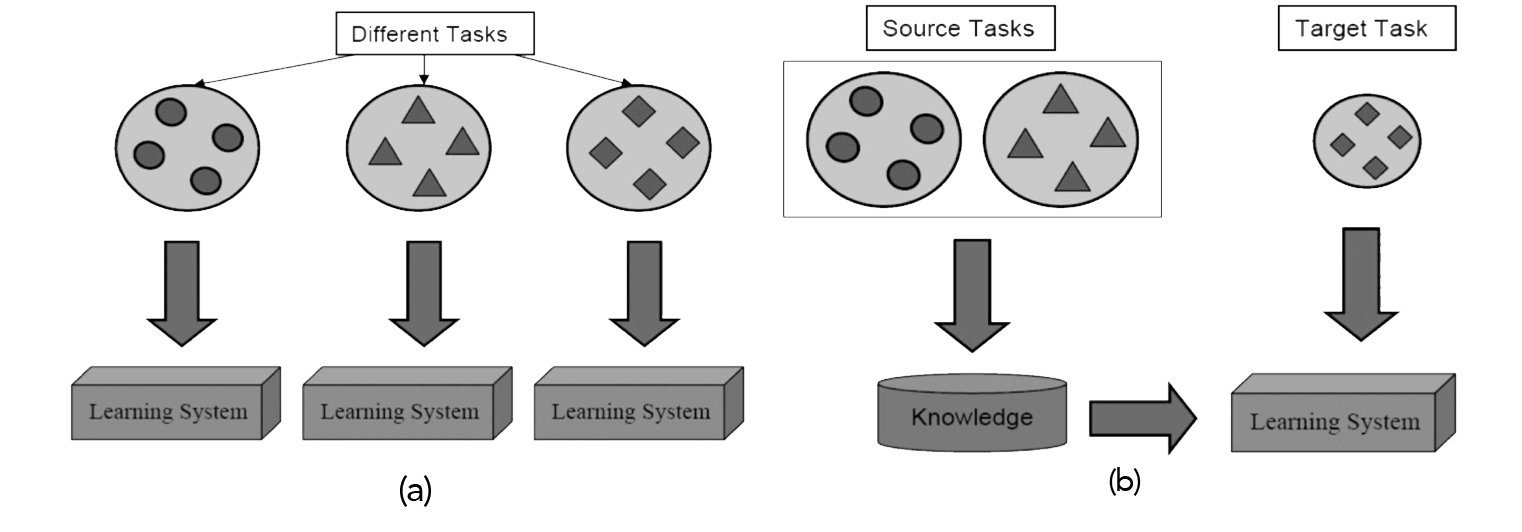
\includegraphics[width=0.8\linewidth]{ml_tl}
		\caption{Difference between traditional machine learning (a) process and feature learning (b) \cite{Pan2010}}
		\label{fig:mesh4}
	\end{figure}
	
	The same idea can be understood from a mathematical point of view as the analysis of the relationship between the two different spaces from types of targets \cite{Pan2010}. 
	
	Considering a \textit{domain} $D$ that is composed by a feature space denoted by $X$ and a marginal probability named $P(X)$, where $X = \{x_1,..., x_n\} \in \chi$. The whole domain can be expressed as $D = \{\chi P(X)\}$ \todo{CPM: no entiendo esta notación, ¿está bien transcrita?} where $x_{ith}$ \todo{CPM: ¿es necesaria la th?. Yo diría  where $x_i$ is the $i{th}$ vector in the feature space} is a certain vector inside the feature space.
	
	In the same way, a \textit{task} can be defined as $T$ formed by a label space $\gamma$ and an objective predictive function $\eta$. The task formulation is $T = \{\gamma, \eta\}\}$ \todo{CPM: aquí falta o sobra una llave}. This predictive function cannot be observed, however the intention is to learn it from the training data, that is composed by pairs of the form $\{x_i, y_i\}$, $x_i \in X$ and $y_i \in \gamma$.
	
	The predictive function $\eta$ can be used to predict a corresponding label of a new sample $x$. From a probabilistic perspective, this new label can be expressed as $P(y|x)$. So, the task $T$ can be defined as $T = \{y, P(Y|X)\}$, in which $Y = \{y_1,..., y_n\} \in \gamma$. For each vector $x_i$, the function $\eta$ finds a prediction $y_i$.
	
	Once these parameters have been defined, considering the source domain $D_S$, task of source domain $T_s$, the target domain as $D_T$ and its respective task as $T_T$, the transfer learning has the purpose of obtain the condition distribution in the target domain $P(Y_T|X_T)$ with the information extracted from $D_S$ and $T_S$ where $D_S \neq D_T$ or $T_S \neq T_T$ \cite{Ruder2017}.
	
	\todo{CPM: aquí añadiría un párrafo diciendo por qué esto es relevante en nuestro problema y en qué lugar de la memoria se sigue con esta idea.}
	
\section{Violent Event Detection}

	All the multimedia information available can be applied to many fields and with different connotations. One of the variants that has appeared in the acoustic scenes and events field is the one applied to violence detection. For this case, an essential point before addressing any problem is to decide what kind of definition the word 'violence' is going to adopt since it is a subjective concept. An objective perspective has been given by the World Health Organization as "The  intentional  use  of physical  force  or  power,  threatened  or  actual,  against oneself, another person, or against a group or community, that either results in or has a high likelihood of resulting in injury,  death,  psychological  harm,  mal-development  or deprivation" \cite{Krug2002}. There are other definitions found in different works as "physical violence or accident resulting in human injury or pain" \cite{Demarty2013} or "any situation or action that may cause physical or mental harm to one or more persons" \cite{Giannakopoulos2006}.
	
	Recent studies have treated this problem in different ways due to all types of conditions that this may take place in. During the last years, the possibility of creating and providing audiovisual content has grown widely, which has led to an enormous variety of topics in which, some of them, could be considered inappropriate for certain  audiences. This is the reason why there have just been done works related to the field of video content analysis and detection of violence. 
	
	In some cases, audio and image features have been combined to address these problem \cite{Giannakopoulos2010}. However, it has been found that sound information could be really useful and a more efficient way of working compared to image, since it is easier to process and the cost is lower. Related works have utilized audio features in the time-domain and in the frequency-domain, similar to the ones explained for \acrshort{asc}, then combined with a normal SVM classifier \cite{Giannakopoulos2006}. Other researches have tried more complicated models with the intention of improving the classification task. It is the case of using \acrshort{dnn}, fed with both image and audio data, which performs the task more efficiently \cite{Ali2018}. Violence detection has also been used for other applications such as video surveillance. For example, one of the scenarios for this purpose consists on preventing violent acts inside elevators \cite{Chua2014}. For this case, the considered dangerous situations are composed of anti-social actions that are likely to happen in this kind of places, concretely, urinating, vandalism and attacks on vulnerable victims, such as women, children or elderly. The framework proposed is based on audio-visual data, but the master classifier is driven by audio, due to the possible subtleness of the scenes that are desired to detect. So, first the audio incident detector triggers the process when a non-silent event takes place. Then, the image processing begins in order to extract information related to who is involved in the action and how aggressive is it. Another utilization of the surveillance approach is its use for the evolution of smart cities \cite{Garcia-Gomez2016}. For this goal, since the system will be implemented in real-life environments, one of the advantages about working with data coming from sounds is the respect for privacy, that, otherwise, using video recordings would be violated.
	
	The difference in these two applications, apart from the task they are addressing, resides on the data they are working with. For violent content analysis, the data usually comes from fictional audio sources as movies or video-games. However, for real-environment systems, the data is extracted straight from actual day-to-day life situations. In this second case, some disadvantages can be appreciated. For example, the signals are not preprocessed, which means the original properties of the sound are not modified so the processing part before classification becomes tougher. Also, the presence of background noise is more common and loudness of some events, as speech, may vary with time \cite{Bautista-Duran2017}. \todo{Makes sense? CPM: it does}

\subsection{Gender-based violence}

	\doubt{Throughout history, women have been subjected to abuse and suffering in many different situations even though in those that were considered as their close familiar environments. They have been bashed, sexually harmed and psychologically miss-treated by those who were supposed to be one of their closest intimates \cite{UnitedNations1989}.}
	
	 In the same way, in the recent times, late studies have shown that 35\% of women from all over the world have been victims of physical or sexual damage \cite{WHO2013}, and 43\% of women from Europe have declared going through some psychological or mental violence at least once in their lives \cite{EuropeanUnionAgencyforFundamentalRights2014}. In this context, it is necessary to define the concept of gender-based violence, which can be described as the set of harmful behaviours that are focused on women and girls just because of their sex, such as female children and wife abuse, sexual assault, dowry-related murder and marital rape, among others. Particularly, violence against women involves any act of verbal or physical force, extortion or lethal denial which has a woman or girl as a target and provokes the physical or psychological hurt, humiliation or irrational privation of liberty and contributes to continue women subordination \cite{Heise1999}. Within this definition, it can be considered that most of the times that these violent situations take place, they are originated due to persons that are supposed to be part of the victims' closest circle of trust, i.e., their husbands or boyfriends. This is called \acrfull{ipv} and it is recognized as a public health problem affecting women across their life span resulting in different undesirable unhealthy outcomes, such as depression, chronic pain and even dead \cite{Beyer2015}.
	
\subsection{Our point of view} \todo{Explicación EMPATIA?}
\label{subsection:our-point-of-view}

	As a contribution to the EMPATIA-TC project\todo{CPM: poner una cita formal al proyecto: Department  of  Research  andInnovation of Madrid Regional Authority, in the EMPATIA-CM research project(reference  Y2018/TCS-5046). } developed by \acrlong{uc3m}, the main goal in this work is to make progress in detecting gender-based violence situations, specifically applied to day-to-day scenes, in which \acrshort{ipv} is likely to be present. One of the parts from the proposed system is composed by wearable devices that the victim can carry to collect diverse types of information and process them to obtain conclusions and increase the efficiency. Among these accessories, we can find a pendant that senses the user's voice and the surrounding audio to analyse what is happening at a given moment. For our purpose, the interesting part resides on achieving auditory data so as to detect violent incidents that consists of sounds already known for characterizing these episodes considered dangerous by the victim.
	
	The definition that is assigned to violence is really important in order to define which audio events should be taken into account. However, considering the subjectiveness of this concept, categorizing violence for every type of user is an extremely difficult task. For this reason, the final idea to answer this question is to make the victim able to decide which kind of hearing events the system must be aware of. In the complete project, this can be carried out by a phone user interface which displays a list of sound events and she has the labour of picking up those that are violent according to her criteria. Since the development of this tool is out of the scope of this work, we have decided to implement a simpler mechanism which will be explained in subsection \ref{subsection:violent-classes}.
	
%\subsection{\doubt{Embeddings}}
%
%	\doubt{It can be easy appreciated in the literature that most of the efforts done by the researches are dedicated to the task of gathering enough data and processing it in order to extract features so that it can be adapted to the final problem. Nowadays, there have been created plenty of resources that ease the solution of these tasks, such as the development of multiple public databases that can be applied to many different problems and the implementation of a lot of software libraries that allow to easy extract the desired features. However, when a new investigation process appears in the machine learning field, one of the first common questions is how and where the data is going to be obtained and how it should be look like.}
	

\section{Databases}

	A main objective was to find a database that allows for building a system with the desired characteristics, so a rich variety of acoustic events is needed with an essential big representation of violent sounds. In the table \ref{table:1} is represented a relation of the different databases that have been considered for the realization of this work.
	
	% Databases table
	% !TeX spellcheck = en_GB
% Databases table

\begin{table}[h!]
\begin{center}
	\begin{tabular}{|| m{5em} | m{12em} | m{17em} ||}
	\hline
	\textbf{Name} & \textbf{Description} & \textbf{Considerations} \\
	\hline\hline
	URBAN-SED \cite{Salamon2017} & 10,000 soundscapes with sound events. Every soundscape contains 1 to 9 sound events with strong annotations. & Events are completely specified but it just contains three interesting types of classes. \\
	\hline
	UPC-TALP \cite{Mapell2012} & It belongs to \acrshort{chil} project, for the \acrshort{aed} task. Isolated acoustic events that occur in a meeting room environment. & Payment is needed to achieve the data and the classes are a little out of our topic. \\
	\hline
	MIVIA: Audio Events Data Set for Surveillance Applications \cite{Foggia2015} & 6,000 events with background noise. & The classes included belong to our topic, but they are just three: glass breaking, gun shots and screams. \\
	\hline
	TUT rare sound events \cite{Fagerlund2017} & Source files for creating mixtures of rare sound events (classes baby cry, gun shot, glass break) with background audio. & Similar problem to MIVIA: just from three interesting classes. \\
	\hline
	IEEE AASP Challenge \cite{Stowell2013} & Composed by ASC and AED. It is formed by two subtasks: OL (Office-live) and OS (Office Synthetic) & Labels for both subtasks are out of our scope since they are likely to happen in an office environment: keyboard clicks, hitting table, etc. \\
	\hline
	TUT-SED Synthetic 2016 \cite{Cakir2016} & Isolated sound event samples were selected from commercial sound effects & The variety of classes is large enough but for our purpose just four of them are useful. \\
	\hline
	VSD benchmark \cite{Demarty2015} & Violent events from 32 Hollywood movies and 86 YouTube web videos, together with high-level audio and video concepts. & Payment is needed to purchase the movies and the videos do not specify the type of violent event \\
	\hline
	AudioSet \cite{Gemmeke2017} & An ontology of 632 audio event classes and a collection of 2,084,320 human labeled 10-seconds sound clips from YouTube videos. & The final pick. Plenty of the videos have more than one audio label but we were able to adapt the data to the problem because of the huge amount of clips. \\
	\hline
	Freesound dataset (FSD) \cite{Fonseca2017} & Filling AudioSet ontology with 297,144 audio samples from Freesound. & This may seem a very good option as well but it is not available yet. \\
	\hline
	\end{tabular}
\end{center}
\caption{Table of studied databases}
\label{table:1}
\end{table}

	
	The last three options shown in table \ref{table:1} are the ones that better suit the problem of this project. \textit{VSD Benchmark} was the first option we chose. Within the two ways of working given, the movies and the YouTube videos, the former was the easiest to use since the annotation specified exactly what kind of violent events were present in the scene and the onset and offset time stamps within the whole film. However, this data is copyright restricted and it was necessary to pay for the contents. The latter was accessible but just indicated the presence of violence, without determining the type of event. Another choice was the \textit{Freesound dataset} because it contains all types of videos so we could extract those classes that are more interesting for us. However, it is still under an annotation process and it is not ready to download yet. As a final conclusion, we decided to go for \textit{AudioSet}, which \doubt{will be explained further on. CPM: recuerda poner la sección específica.}.
	
	


\chapter{Resources and Methods for Acoustic Violent Detection}
% !TeX spellcheck = en_GB

	In this chapter we are going to explain the different resources we have chosen to create an approach that allowed us to implement our final models. First, we include a detailed description of the database that we have chosen in section \ref{section:audioset}. Then, we comment and analyze the system we are going to employ so as to obtain high level features for our classification experiments in section \ref{section:feature-extractor}. In this point, the model is itemized step by step and also a theoretical explanation is included in \ref{subsection:ann-cnn}.
	
\section{Database: AudioSet}
\label{section:audioset}

\subsection{What is AudioSet} \todo{How cite? CPM: como misc, por ejemplo en la página web y con el artículo que la describe}
\label{subsection:what-is-audioset}

	Audio Set can be described as a large-scale sound dataset with the goal of putting the availability of audio and image data on the same level. It is composed by a huge variety of 2,084,320 manually-annotated audio events in video format and it is organized by following an ontology formed by 632 different audio classes. The data has been extracted from YouTube videos and the labelling process has been based on diverse factors such as metadata, context and content analysis. It has been developed by Google with the purpose of producing an audio event recognizer that can be applied to plenty of acoustic situations coming from the real world \cite{Gemmeke2017}.
	
	Due to some limitations found during the building process that will be explained along the section, the current final release of the dataset is composed by 1,789,621 segments, where each video usually last 10 seconds which results in a total duration of 4,971 hours of video and audio. After executing the selection process in which the different labels were populated with the final corresponding segments, a total of 527 classes were gathered, out of which 485 counted with at least 100 samples.

\subsection{Ontology}
\label{subsecition:ontology}

	In order to put this dataset together the events have been organized in an abstract hierarchy. This is composed by higher-level classes which describe a certain type of sound event and also act as parents of other labels that refer to more specific events. With this purpose, the relationship among different classes needs to be non-exclusive, so labelling similar audio events may result into a more general class, the parent, if there was ambiguity. This is also helpful for labellers due to group the clips in an easier and faster way.
	
	The Audio Set Ontology was collected considering some fundamental guidelines explained below:
	% List
	% !TeX spellcheck = en_GB
\begin{itemize}
	\item \doubt{A complete collection of all labels must be prepared} so that it can be used to define sound events from real-world aural data.
	\item When labelling an audio event the result must match the criteria of a common listener.
	\item Different categories should be easy to distinguish by an ordinary listener. In the case that two different labels do not satisfy this requirement, these should be merged. With this condition, the spectrum of possible labels remains limited.
	\item The distinction of two different classes must be done by relying just on the audio, it cannot be accompanied by image or visual information.
	\item The hierarchy should not be very deep by keeping the number of children per parent class to no more than 10. This also eases the annotation labour. 
\end{itemize}

	
	It is easy that an ontology of this volume gets leaned or biased towards a particular direction due to several factors, such as the subjectiveness of its creators or the selection of the initial set of classes used when starting to label. With the intention of generating a primary list that covers a wide range of audio events in an objective way, the researchers decided to apply an impartial, web-scale text analysis from the very beginning. They agreed on detecting hyponyms of the word "sound" by utilizing a modified version of the famous technique called \textit{Hearst patterns} \cite{Hearst1992}, a method proposed to automatically acquire hyponymy lexical relations from unrestricted text. As a result, an enormous collection of terms came up. This was filtered by considering how well these terms represented audio, i.e. by combining together the global frequency of occurrence and how exclusively these are recognized as hyponyms of "sound" instead of other terms. As an output of the final process, a list of 3000 terms was obtained.
	
	With respect to the hierarchical relation among categories, it was constructed by the authors with the main intention that this satisfied their human comprehension of the sounds. Event though this is a subjective manner, it also makes sense since this is how the hierarchy best performs its labour on helping human labelling.
	After all the organization process, the model is not based on a strict organization as a singular node can appear in many different locations, i.e., a single node can be child of different parent nodes. As we said before, the final result is composed by 632 audio event labels and, in the hierarchy, the deepest class is six level away from the top parent. Figure \ref{fig:mesh1} shows the nodes that belong to the two top layers of the ontology.
	
	% Figure of ontology
	\begin{figure}[h]
		\centering
		\captionsetup{justification=centering}
		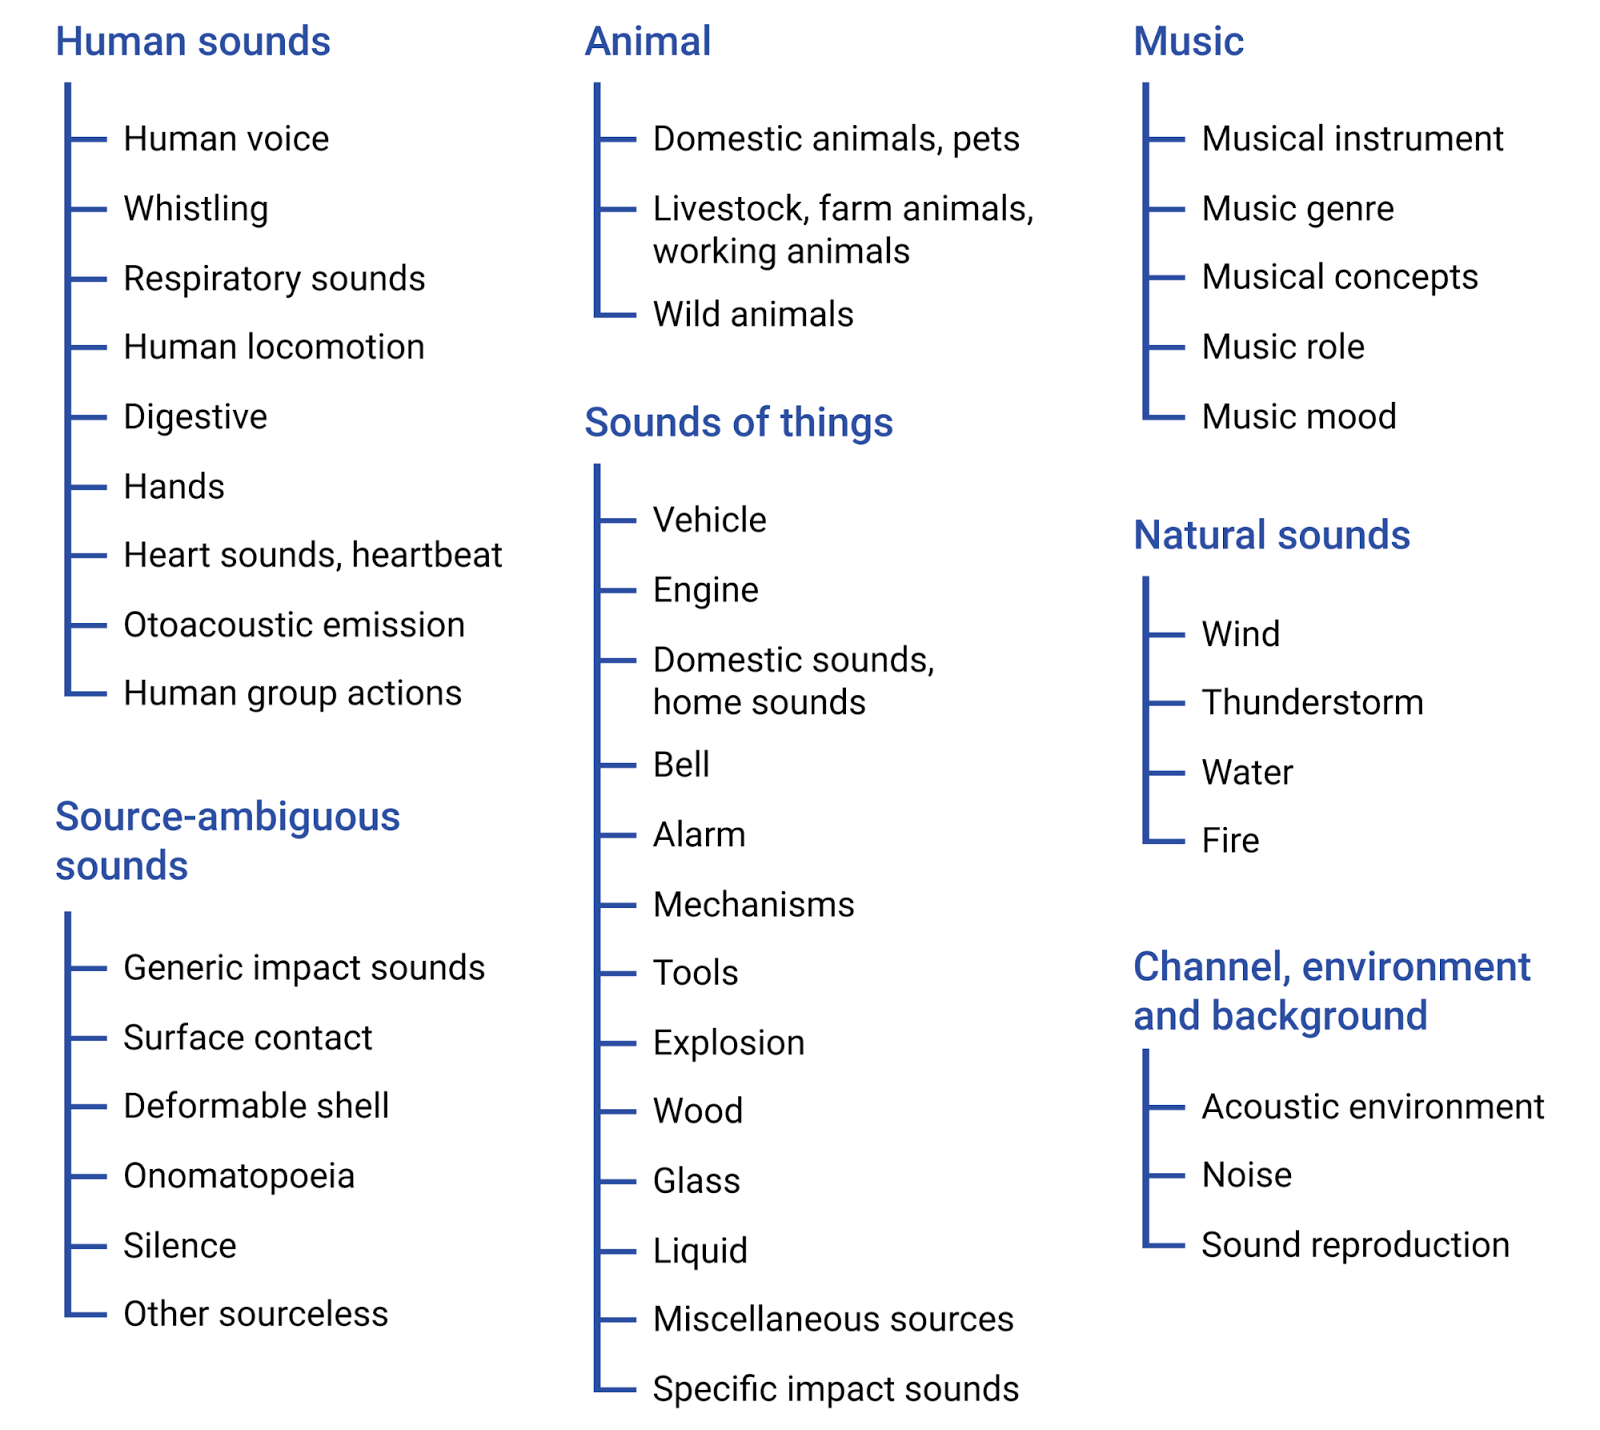
\includegraphics[scale=0.21]{audioset-ontology}
		\caption{First two layers of Audio Set Ontology \cite{Gemmeke2017}}
		\label{fig:mesh1}
	\end{figure}
	
	This whole structure is offered to any user as a file in JSON format. A couple of fields have been included for each label in order to describe its meaning and make clear its position within the hierarchy. A description for all of these can be found in table \ref{table:2}. 
	
	% !TeX spellcheck = en_GB
% Ontology-fields table

\begin{table}[h!]
\begin{center}
	\begin{tabular}{|| m{7em} | m{22em} ||}
		\hline
		ID & This field includes the Knowledge Graph \acrfull{mid} that best describes the sound or its source. It is used as a primary identifier for the class. \\
		\hline
		Display name & Short name formed by one or two words that identifies the audio class. It sometimes includes a small alternative separated by a comma so it does not feel ambiguous. \\
		\hline
		Description & One or two explaining sentences so the meaning of the category is more defined. These can be extracted from Wikipedia or WordNet. \\
		\hline
		Examples & At least one example of the label is provided as a URL of a YouTube video. \\
		\hline
		Children & An array filled by the \acrfull{mid}s from all immediate children of the class. \\
		\hline
		Restrictions & It specifies if the category in question either has been discarded or there are no audio clips under it. \\
		\hline
	\end{tabular}
\end{center}
\caption{Fields per category in the ontology.}
\label{table:2}
\end{table}
	
	For the field \textit{ID}, the identifiers are known as \acrfull{mid} and belong to the \textit{Knowledge Graph} designed by Google \cite{Singhal2012}. This is a knowledge base that Google services use to improve the quality of its search results and it is composed with information extracted from a wide variety of sources. The \acrshort{mid}s are the identifiers of the different elements that belong to this huge dictionary. For instance, the \acrshort{mid} of the word "Speech" is "/m/09x0r". Another field that deserves a special explanation is the one corresponding to \textit{Restrictions}. Within all the categories of sound events, there are two flags that indicate an exclusive behaviour that differ from a typical label: "blacklisted" and "abstract". The former refers to a class that has been hidden from labellers due to its confusing meaning. The latter has been used for those classes that are just employed as intermediate nodes in order to provide a better grouping inside the organization, and are not expected to be used in the implementation tasks. In total, out of the 632 categories, 56 have been categorized as "blacklisted" and 22, as "abstract".


\subsection{Data access}
\label{subsection:data-access}

	The data can be obtained through the website \cite{SoundUnderstandinggroup2017} in two different formats:

	\begin{itemize}
		\item Files in \acrshort{csv} format that include for each video segment its YouTube video ID, start time, end time and the one or more labels it belongs to. 
		\item Instead of the audio files themselves, they provide already extracted audio features for each segment in compressed files that are available in \acrfull{tf} \cite{GoogleResearch2015} record files that can be easily downloaded.
	\end{itemize}
	
	Together with these two options of obtaining the data, a neural network model is also provided in the database website which can be used to extract embeddings as high-level features. It is called \textit{\acrshort{vgg}ish} \cite{Hershey2017} and it has been pre trained on a preliminary version of the database YouTube-8M \cite{Abu-El-Haija2016}. A more detailed explanation of this system is later included in \ref{subsection:vggish}.
	
	Based on the first choice, we did some attempts of downloading a couple of videos from YouTube using the information given in the \acrshort{csv} files. Then, we decided to try to extract our own embeddings features by running the \acrshort{vgg}ish network with the downloaded videos in order to see how they look and check their behaviour on a classification task. Also, for the second option, we downloaded the provided embeddings already extracted by the Google developers and see if they were also useful for our problem. A little experiment explained in \ref{subsection:exploring-differences-between-two-types-of-data-access} were implemented so as to check if the two manners of obtaining the embeddings were equivalent.

\section{Feature extractor}
\label{section:feature-extractor}

	\acrshort{vgg}ish model design was based in an already existed network called \acrshort{vgg}. In order to describe the embedding features extractor we used, it is first needed to make a clear explanation of what a \acrlong{ann} is and how \acrlong{cnn} behave. Then, an explanation about how the \acrshort{vgg} model is implemented included. Then, we can move to analyze the differences and changes included in \acrshort{vgg}ish. 

\subsection{\acrlong{ann}s (\acrshort{ann}) and \acrlong{cnn}s (\acrshort{cnn})}
\label{subsection:ann-cnn}

	Before going deep in the description of \acrshort{cnn}, the core idea of \acrshort{ann} must be explained. As it was already mentioned at the end of subsection \ref{section:features-and-methods-for-asc-aedc}, these are based on the communication way that the neurons follow inside a brain to interpret the stimuli they receive. This is actually the hidden concept behind the \acrshort{ann} intention, which is transforming input data into a desired output so that it can be used to perform a given task. %it can understandable by a machine. 

	A basic architecture is usually composed by an \textit{input layer} of neurons, a certain number of \textit{hidden layers} and an \textit{output layer}. The model receives some input, typically a feature vector, and pass it trough the hidden layers in order to perform some transformations. The neurons of a layer are completely connected to the neurons of the next layer but neurons in the same layer are not usually connected. For this case, we can say that they are \acrfull{fc} layers. Finally, the output layer gives the resulting outcome of the network \cite{Kwon2011}. This is just the basic and initial nature of the idea but it was implemented in many different ways depending on the input data and the desired task.

	Within the different possibilities of designing an artificial neural network, there are two main options. The selection of one of them depends on the complexity of the problem, the format of the input data and how it is combined with other techniques. One of them covers all the models that are structured with a shallow architecture. An example of this would be a basic type of network known as \acrfull{mlp} that follows the structure explained for \acrshort{ann} with \acrlong{fc} layers but composed just by one hidden layer. This type of systems have performed well in many tasks but they have shown some limitations in more complicated applications \cite{Deng2014}.

	When working in real-world cases such those that involve natural signals, such as human voice, natural sounds and visual scenes, for example, it is needed the development of a deeper architecture in order to extract and understand the complexity inside this type of data so as to build. For example, visual and speech recognition tasks are exploited with system that follows the hierarchical transformations that the humans perform when understanding this type of data. reliable and useful internal representations. This type of models are collected inside the \acrfull{dnn} field. \acrshort{dnn} has been one of the most studied fields since it was proposed in 2006 \cite{Deng2014}. In figure \ref{fig:mesh48}, it can be found a comparison between shallow and deep models.

	\begin{figure}[ht]
		% Whole figure
		\captionsetup{justification=centering}
		\begin{subfigure}[b]{\textwidth}
			% Start with figure wav
			\centering
			\captionsetup{justification=centering}
			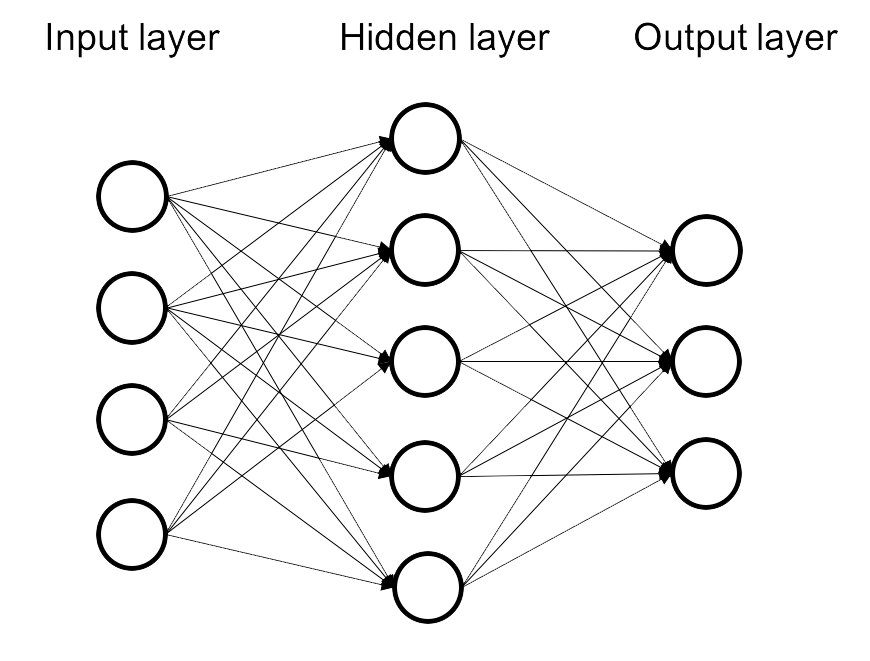
\includegraphics[width=0.45\linewidth]{shallow}
			\subcaption{Shallow architecture}
		\end{subfigure}
		\vskip\baselineskip
		% Start with figure tfrecord
		\begin{subfigure}[b]{\textwidth}
			\centering
			\captionsetup{justification=centering}
			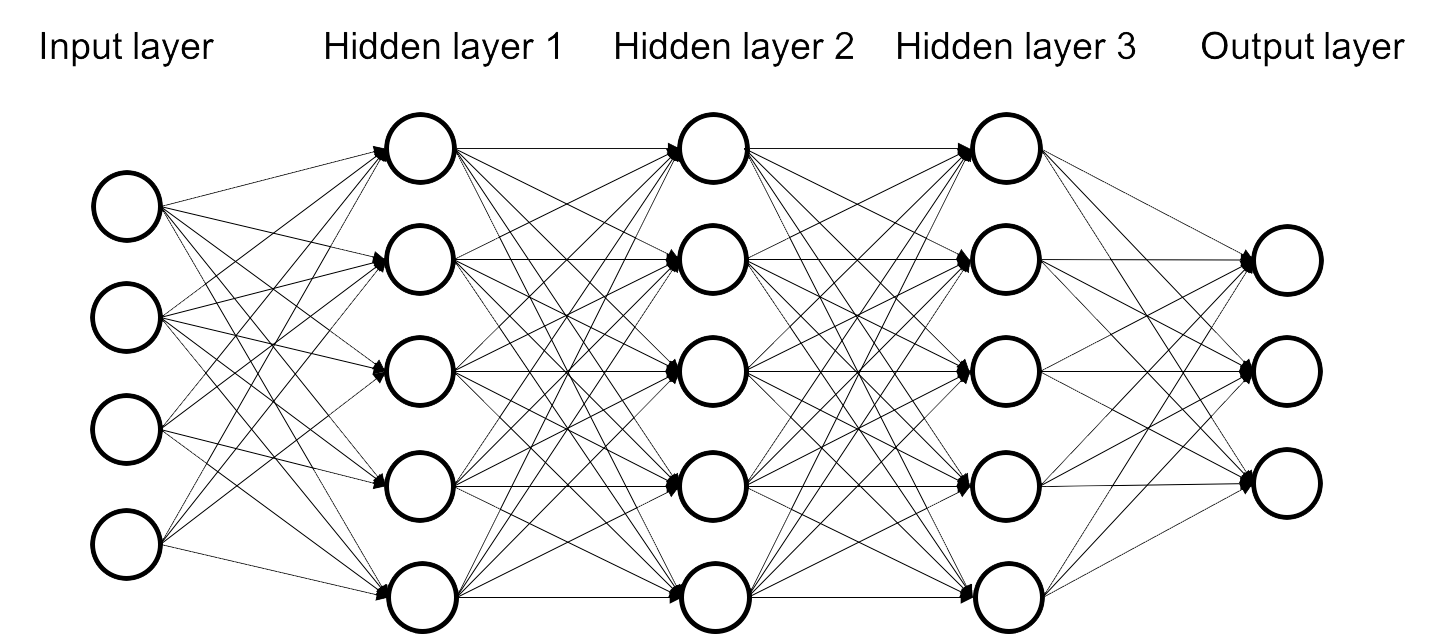
\includegraphics[width=0.6\linewidth]{dnn}
			\subcaption{Deep architecture}
		\end{subfigure}
		
		\caption{Comparison between shallow networks and deep neural networks \cite{Di2018}}
		\label{fig:mesh48}
	\end{figure} 

	% !TeX spellcheck = en_GB
% CNN explanation

\label{section:cnn}

	One of the most explored implementations is the one related to \acrfull{cnn}. This maintain the basic idea of receiving some inputs and apply a dot product operation to them before subject the data to a non-linear function but with the difference that input data are expected to be images \cite{Karpathy2016}. The architecture of a \acrlong{convnet} is based on the organization of the Visual Cortex in the human brain. This means that single neurons responds to some stimuli only in a certain region of the visual field, the Receptive Field. Then, a collection of these fields overlap with each other so as to cover the full visual space \cite{Saha2018}.
	
	About the input data, it is introduced as a matrix instead of as a row vector. Then, the architecture of the layers adapt to the fact that input data are images. They do not consist of a single row of neurons, but they have a shape constituted by three dimensions: heigh, width and depth \cite{Karpathy2016} \todo{include image?}. In this way, the net can capture the spatial and temporal relations present in an image by applying some filter functions. With this construction, the model can be trained with a smaller number of parameters and also reuse the weights.
	
	A \acrlong{convnet} can be described as a sequence of layers in which every layer converts a volume of activation results from the previous layer to another by computing a differentiable function. The architecture of a \acrshort{cnn} is always composed by three type of distinguishable layers which are \textit{Convolutional}, \textit{Pooling} and \textit{\acrlong{fc}}. A normal architecture will follow the next succession of layers \cite{Karpathy2016}:
	
	\begin{itemize}
		\item INPUT: this represents the image at the entrance of the whole model. It commonly is a 3\acrshort{d} matrix , one dimension per channel of colour, and contains the values of the original pixels.
		\item CONVOLUTIONAL: considering the neurons that are connected to a region of the input image, this layer computes their output by performing a dot product between the weights and the value of the pixels. The depth of the resulting data will coincide with the number of filters used.
		\item POOL: this performs a fixed operation that consists of a downsampling of the spatial dimension. It typically reduces by half the height and the width of the input image.
		\item \acrshort{fc}: this is the final layer which gives the output of the whole net. It is a vector-shape layer and is completely connected to the previous layer. In a classification task the number of neurons matches the amount of classes of the problem.
	\end{itemize}
	
	Note that this list represents the order of the layers in the architecture, however, the number of layers of each type vary depending on how the model is designed and how deep it is desired to be. For example, some examples of deep architectures can be found later in section \ref{subsection:vgg}, in table \ref{table:3}.
	
	With this building, a \acrlong{convnet} passes the information of the pixels layer by layer while reducing the input images in a way that is much easier to process. This is performed without missing any feature since all of them are essential to compute a good prediction outcome.
	
	In the convolutional layer, a convolution operation is performed for each small region of the input image. The element that carries out this operation is called \textit{kernel} or \textit{filter}. This partial region that the kernel covers in the input data is set by deciding the height and the width as a designing parameter. About the depth, it must match the depth of the input data so the filter can slide trough the image along its 2\acrshort{d} and obtaining the results of the convolution operation by computing between the pixels inside the region and the values of the filter. An example can be observed in figure \ref{fig:mesh11}. For each filter, a 2\acrshort{d} activation map is obtained after subjected the result of the convolution to a non-linear operation as the \acrfull{relu} function. Finally, we will pack all these in a unique volume that will consists in the output of the convolutional layer \cite{Karpathy2016}. For example, if we have a number of 64 filters, we will get then a group of 64 2\acrshort{d} activation maps that will be the input of the next layer. Traditionally, it was the first convolutional layer the one that was responsible of capturing low-level features related to edges or colours in the image. The upper layers were the ones in charge of extracting high-level features so the network was able to understand the image similar to how the humans do \cite{Saha2018}.
	
	\begin{figure}[ht]
		\centering
		\captionsetup{justification=centering}
		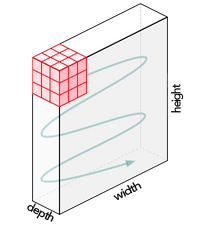
\includegraphics[scale=0.6]{movement-of-kernel}
		\caption{Movement of the kernel represented as a red block along the width and the height of the original input image. It is clear that it occupies the whole depth of the input image. The arrow indicates an approximation of the movement that the filter follows \cite{Saha2018}.}
		\label{fig:mesh11}
	\end{figure}

	We have included how the input interacts with the convolutional layer and also introduced the concept of depth of the resulting volume. However, it is needed to explain the how the total size of this output is computed and what it depends on. There are three main parameters that play a role in this decision: \textit{depth}, \textit{stride} and the \textit{zero-padding} \cite{Karpathy2016}.
	
	\begin{itemize}
		\item DEPTH: it is a hyperparameter that corresponds to the amount of kernels used in the convolutional layer when learning from the input.  The set of neurons that extent through the depth dimension operating in the same region is called depth column. This is the previous mentioned red block shown in figure \ref{fig:mesh11}.
		\item STRIDE: this indicates the displacement of the sliding filter along the image. If it has a value of 1 (non-strided), this means that the kernel will shift a position of one pixel along the width. When it is set to 2, then it moves two pixels. It rarely has values greater than 2. The moving process consists on the filter going from right to left with a hop determined by the stride value. When the right margin is reached, then it jumps to the beginning of the next row from the left margin and repeats the process in the same way until the image is completed \cite{Saha2018}. The bigger the stride, the smaller the size of the output volume.
		\item ZERO-PADDING: this is also called just \textit{padding}. It consists on adding zeros to the borders of the image. What is a hyperparameter in design is the size of this padding. This allows to control the width and height of the output volume so we can keep it the same through the different layers. When it is indicate a "valid padding", it means that no padding is added and the output size will be reduced. If we indicate "same padding", then it has a value of 1 and means that the resulting volume will have the size of the input \cite{Keras}.
	\end{itemize}

	As shown below, the total size of the obtained volume, $D$, can be computed as function of the input size, $W$, the spatial 2\acrshort{d} dimensions of the convolutional filter, $F$, the stride of the filters shifting, $S$,  and the amount of padding in the zero-padding, $P$ \cite{Karpathy2016}. 
	
	\[ D = \frac{W - F + 2P}{S} + 1 \]
	
	The convolutional layers can be grouped all together, one after another, but they are usually interpolated by what it has been previously defined as \textit{pooling} layer. This habit has the objective of reducing the the width and the height of the resulting volumes in a progressive manner in order to decrease the total number of training parameters and control the computational cost, and, therefore to avoid overfitting \cite{Karpathy2016} \todo{Include definition of overfitting or just cite it}. There can be performed two types of pooling operation: the max-pooling or the average-pooling. The former just returns the maximum value from the portion of the image where the filter is placed. The latter, computes the average of all the values in this portion \cite{Saha2018}. The pooling layer acts in an independent way on every input depth level. 
	
	Two hyperparameters are needed in order to configure the spatial portion in which the pooling is computed: the  filter size, related to length of height and width, and the stride. However, for this operation zero parameters are introduce since it consists on a fixed operation over the input data. In figure \ref{fig:mesh12}, it is shown how the max-pooling operation is performed \cite{Karpathy2016}. 
	
	\begin{figure}[ht]
		\centering
		\captionsetup{justification=centering}
		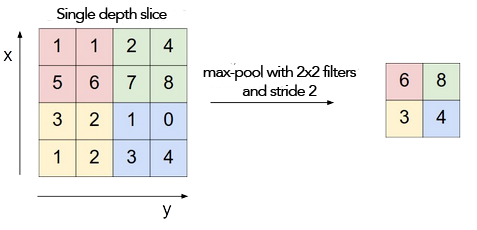
\includegraphics[scale=0.7]{max-pooling}
		\caption{Max-pooling operation with a filter size of 2 and a stride of 2 for a single depth filter. Each colour represents a the action portion for each operation \cite{Karpathy2016}}
		\label{fig:mesh12}
	\end{figure}
	
	Together a convolutional layer and a pooling layer constitute a complete layer structure typical in a \acrlong{convnet}. The number of these complete layers can vary depending on the design and the task needs. These represent the main core of the network before passing to the last layers and calculating the final output \cite{Saha2018}.
	
	For the final step, a common way of acting is to apply some non-linear activations in order to learn from the high-level features resulted from the output volume of the last convolutional layer. This takes place in the \acrlong{fc} layers ending the model. This part has the shape of a Fully-Connected layer, as the one described in the basic model of \acrshort{ann}. To make the weights from the convolutional layers available to feed this last part of the model, it is necessary to flatten the output volume and obtain a column vector. The learning process is possible due to a backpropagation operation performed in every epoch of training. As a total output, the values that represent the classification of the different samples into one or another category are obtained \cite{Saha2018}. A common classification technique is the one called \textit{Softmax}. This normalizes the result of the previous \acrshort{fc} layer into a vector whose values follow a distribution that total sum results in 1. This type of output is called \textit{soft predictions} and represent the probability for each sample of belonging to a category in the classification \cite{Mahmood2018}. However, there exists other activation functions that can compute the classification output in other ways. 
	
	In figure \ref{fig:mesh13} an scheme of a common \acrlong{cnn} is shown. This takes an input image, compute the features along three groups of convolutional layer plus max-pooling and, finally, includes three \acrlong{fc} layers, being the last one a softmax function layer with as many neurons as classes that gives the soft predictions for this image of belonging to each class.
	
	\begin{figure}[ht]
		\centering
		\captionsetup{justification=centering}
		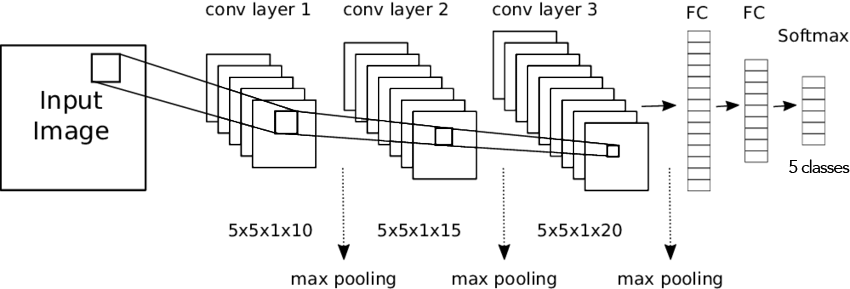
\includegraphics[scale=0.4]{cnn}
		\caption{Representation of a typical CNN model \cite{Hinz2016}}
		\label{fig:mesh13}
	\end{figure}

	\acrfull{cnn} were originally designed to work with images but they have been applied to other fields as audio. An image can be defined as a matrix of values, i.e. pixels, in two or three dimensions, so the only prerequisite to use a \acrshort{cnn} is to have the input data in this form. For audio researching, it has been commonly used the log-scaled mel spectrogram, that is a way of representing audio in a scale different than frequency that is more similar to humans perception. It has been used in plenty of works with \acrshort{cnn} and also combined with other techniques \cite{Salamon2017} \cite{Piczak2015} \cite{Kumar2017}.
	
	
	

	

	
	
	
	
	


\subsection{\acrfull{vgg} model}
\label{subsection:vgg}

	\acrshort{cnn} are usually able to achieve really good results and even improve human skills on \acrlong{cv} tasks, for example, on recognizing object in an image. With the exponential growth of the researching works on this field, some challenges have appeared so as to promote the creation of new systems and test their efficiency and results. This is the case of the \acrfull{ilsvrc}, based on the database of the same name, ImageNet. As a solution for the proposed exercise, the investigators from the \acrfull{vgg} in the University of Oxford implemented a new system achieving the first position and winning the challenge in 2014 \cite{ImageNet2014}. The work they proposed consists of a study of the depth in a \acrlong{convnet} architecture and how this can affect to the accuracy on the goal of large-scale image recognition \cite{Simonyan2015}. To try this, it was necessary to increase the number of layers in the network, which was viable due to use a small size of convolutional filters in all of them.

	For the training step of their system, they used an input image with standard size of $224 \times 224$ in \acrshort{rgb} format. The principles to build the architecture are detailed below:
	
	\begin{itemize}
		\item The input image crosses a bunch of convolutional layers in which the kernel has a size of $3 \times 3$.
		\item The convolutional stride has a value of 1 pixel.
		\item The padding is fixed to 1 pixel, so the dimensions of the input do not change during the convolution.
		\item Max-pooling is also included with a window size of $2 \times 2$ and a stride value of 2 pixels.
		\item Two \acrfull{fc} layers with 4096 channels after all the \acrlong{convnet} layers.
		\item One \acrshort{fc} layer with 1000 channels to perform the \acrshort{ilsvrc} classification.
		\item A soft-max layer is employed for the final layer.
		\item All hidden \acrlong{convnet} layers use the non-linear function \acrshort{relu} as activation function.
	\end{itemize}
	
	All the designs that the creators came up with are based on these initial guidelines, except from just one case where \acrfull{lrn} is applied, previously mentioned in subsection \ref{subsection:ann-cnn}. They just differ from each other on the number of layers, starting with 11 the first approach and ending with 19 the last one. The different architectures are specified in the table \ref{table:3} \cite{Simonyan2015} and are ordered from A to E.
	
	% Table configuration of VGG
	\begin{table}[t!]
		\begin{center}
			\captionsetup{justification=centering}
			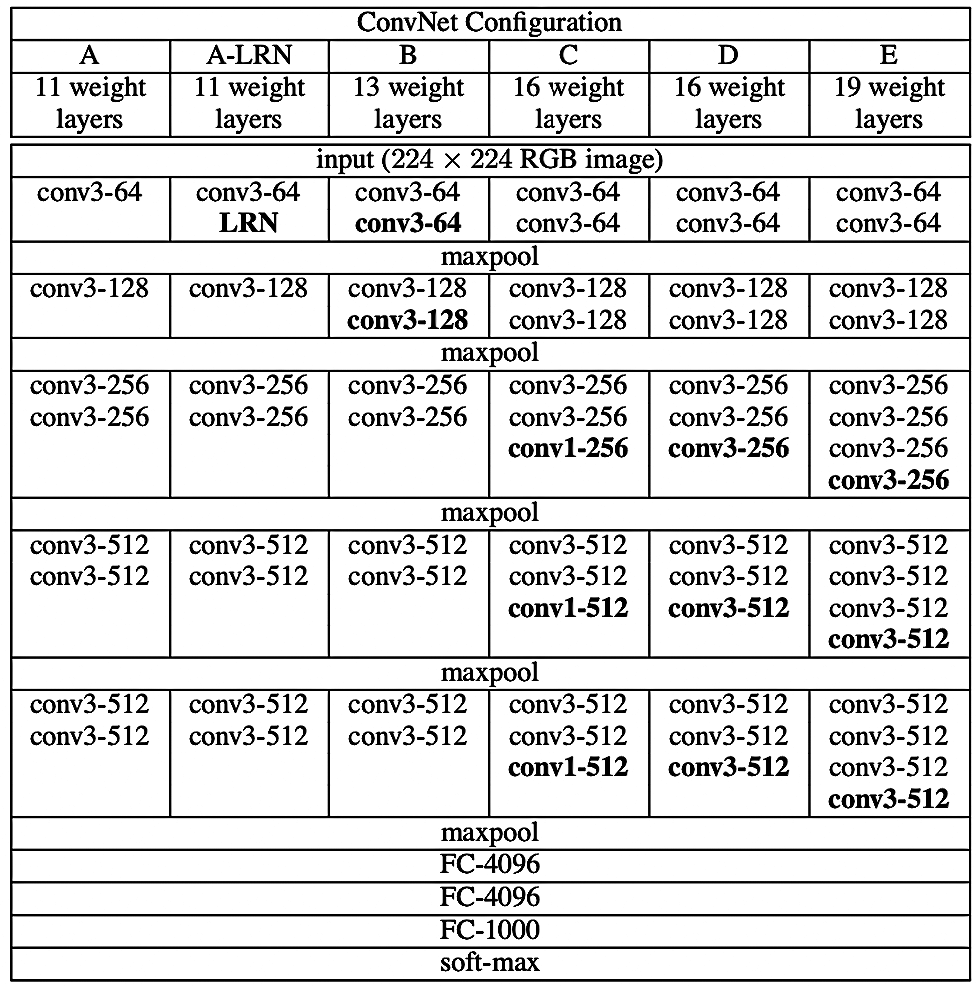
\includegraphics[scale=0.4]{vgg-confs}
			\caption{VGG ConvNet configurations.}
			\label{table:3}
		\end{center}
	\end{table}

\subsection{\acrshort{vgg}ish model}
\label{subsection:vggish}

	The model we used in our project for feature extraction presents a configuration with principles similar to the ones explained in the previous subsection \ref{subsection:vgg} but with slight changes that their developers have included in order to adapt it to the audio approach. As previously mentioned in subsection \ref{subsection:data-access}, the implementation of this model has been obtained from the website of the database Audio Set, in which a code repository is public available \cite{Ellis2017} and all the information about the implementation is included.
	
	The architecture is based in the configuration A from table \ref{table:3} with 11 weights. The differences respect to the original network are listed below: 
	\begin{itemize}
		\item The input size was changed from $224 \times 224$ to $96 \times 64$ because of the log-mel spectrogram audio inputs.
		\item They built the implementation with just four groups of convolutional and max-pool layers, instead of five.
		\item For the last \acrshort{fc} layer, they decided to build it just with 128 channels since it is the layer that compacts the final embedding and defines its dimensions.
		\item Also the final \textit{Softmax} layer is not used.
	\end{itemize}
	Figure \ref{fig:mesh2} shows how the configuration of the final \acrshort{vgg}ish model looks.
	
	\begin{figure}
		\centering
		\captionsetup{justification=centering}
		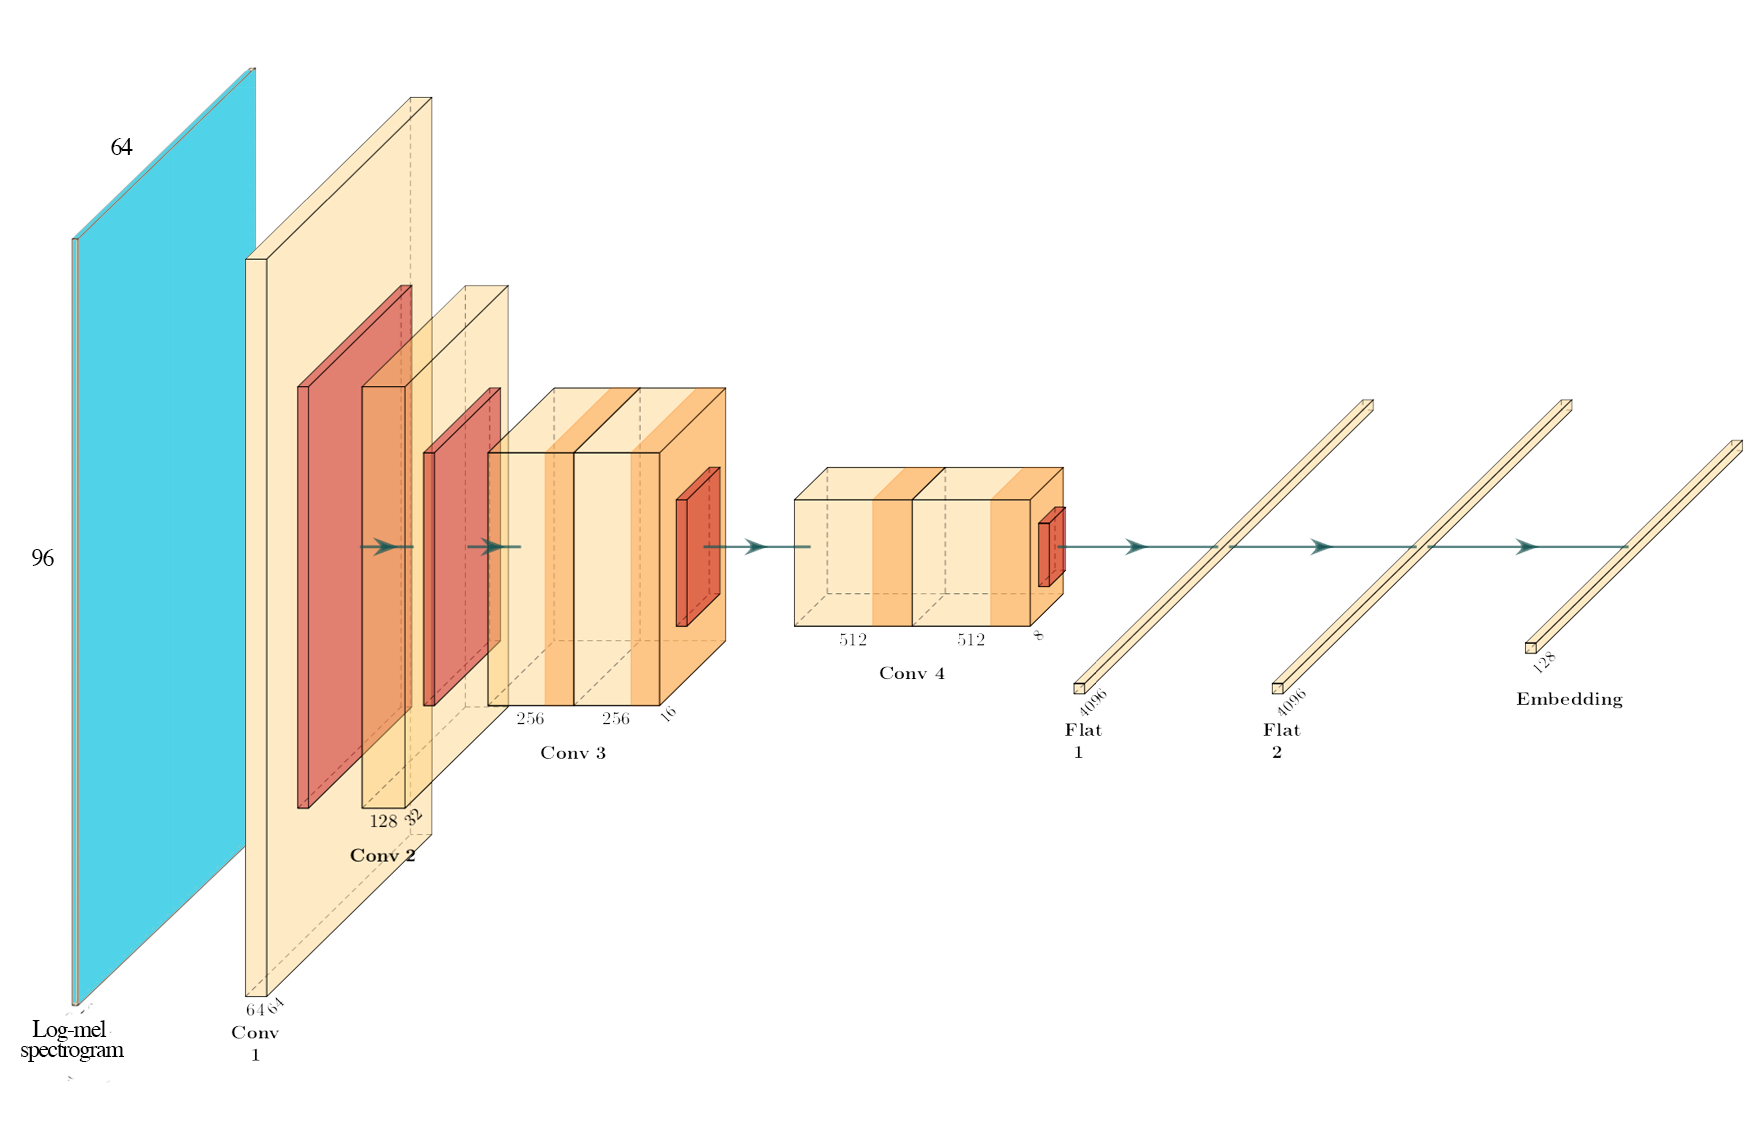
\includegraphics[scale=0.25]{model-vggish}
		\caption{VGGish architecture}
		\label{fig:mesh2}
	\end{figure}

\subsubsection*{Input stage}

	Before passing the data through the whole \acrshort{cnn}, a preprocessing stage has been included by the developers in which the input audio will suffer some transformations. 

	\begin{enumerate}
		\item In the first place, after loading the input audio, the sample rate and the number of channels are checked to be 16 kHz and monochannel, otherwise the file is transformed to satisfy these conditions.
		\item When the data is ready, the next step is computing the spectrogram. For this, it is necessary to calculate first the \acrfull{stft} of the signal. The operation is performed by using a sliding Hanning window of 25 ms with a hop size of 10 ms. As a result, just the magnitudes that correspond to the positive frequencies are retained, since the ones corresponding to the negative part of the spectrogram are redundant.
		\item  Transforming the spectrogram to Mel scale is what follows. To do so, they compute all mel frequency bins that are going to modify the values of the spectrogram in frequency domain by following a hertz to mel conversion formula, that can be found in appendix \ref{section:spectrogram-mel-scale}. The result is a mel spectrogram from 125 Hz to 7,500 Hz divided in 64 bins.
		\item Then, the log-mel spectrogram is calculated by doing the logarithm of the previous result plus a small offset value to avoid the logarithm of $0$.
		\item As a final step, they compute a framing operation over the log-mel spectrogram. The resulting are non-overlapping examples of 0.96 seconds, in which 64 mel bands and 96 frames are contained, each frame with a duration of 10 ms.
	\end{enumerate}

	Therefore, the result obtained is an ensemble of 10 frames, approximately one per second, each of them with size $96 \times 64$, i.e, 96 frames and 64 mel bands.

\subsubsection*{Embedding stage}

	Once the initial processing part is done and the log-mel spectrogram matrix is computed and divided into the desired number of frames, it is used as input data for the \acrshort{vgg}ish \acrshort{cnn}. After all the computations inside the network, each example is converted into an embedding of size 128 giving a result of one of these per second of the original audio file.

\subsubsection*{Postprocessing stage}

	As final step, they performed some post-processing of the resulting embeddings. A \acrfull{pca} \cite{Abdi2010} transformation is done joint with a whitening process. Also, a quantization to 8 bit for each embedding element. All these actions are computed with the purpose of making the final output compatible with the embeddings obtained from the YouTube-8M database.

	\todo{Transfer learning and why choosing this type}


\chapter{Our approach for Acoustic Violent Detection}
% !TeX spellcheck = en_GB

	In this chapter we want to make clear why we think that the \acrshort{vgg}ish network is a good option for our problem in \ref{section:why-vggish}. Then, the procedure when starting to prepare the data and to extract the feature embeddings with this model is included in \ref{section:our-approach}. Also, the demonstration of the similarity between both types of embeddings previously mentioned in \ref{subsection:data-access} is described in \ref{subsection:exploring-differences-between-two-types-of-data-access}. Finally, the last section \ref{section:models} includes an explanation of the different algorithms that we use for the experiments explained in chapter \ref{chapter:experiments}.

\section{Why \acrshort{vgg}ish}
\label{section:why-vggish}

	For our goal, one of the toughest tasks consisted on the selection of data that properly adapted to our problem and its preparation so as to obtain features that allowed us to characterize every acoustic event from a violent point of view. Since our first efforts of finding an available dataset containing enough violent scenes was driving us to a dead end, we decided to take advantage of a huge database which let us rethink the standpoint about how we were going to address the problem. As it was mentioned in subsection \ref{subsection:our-point-of-view}, one of the main questions was how to define the term violence for each victim depending on  her certain situation. After finding the Audio Set database, previously explained in section \ref{section:audioset}, with all its variety of samples, we had a wide range of audio data to work with. This is how we came up with the system explained below in \ref{subsection:violent-classes}.

	At this point, not only we had an idea but we had already found a data resource to start with. However, the issue was related to what kind of features could be extracted in order to categorize events from different nature with a unique violent label. An acceptable conception of the term violence could be expected to cover all kinds of impulsive events such as hits, smashes, gunshots, yells, etc. Also, we would like to introduce sounds that were likely to happen in a domestic environment within a tense atmosphere as children crying, dog barking or glass breaking. We also wanted to take into account the possibility of including other cases not usually considered violent a priori. For example, the sound of keys jangling or the noise produces by a shaver machine. These situations may be too particular and just would be present in few uses, but this is how we understand the problem given the advice of the social sciences experts in the UC3M4Safety team.

	So, our first intention was to apply some audio processing techniques to extract low-level features, as the ones previously explained in \ref{subsection:features-and-methods}. Even though there are plenty of previous works and a lot of tools to work in this way, it was not sure which path should we take in order to decide what features better fitted our task. Apart from this, since the database had such a big volume it would have supposed an enormous cost of time to compute features every time we wanted to try new type of categories. Moving on, by following the advances on finding new level features already mentioned in \ref{subsection:features-and-methods}, we decided to investigate new methods of extraction based on the use of \acrlong{nn} models. Nevertheless, even thought the features obtained in this case had been more appropriated, the time consumption of training a big model was one of the aspects that did not totally convince us.

	The previous selection of Audio Set as our dataset allowed us to get to know the \acrshort{vgg}ish model proposed by Google researchers for feature extraction. This system loads the parameters already learnt from training with another huge dataset as YouTube-8M. This is possible due to apply transfer learning idea, explained above in subsection \ref{subsection:transfer-learning}, that consists of leveraging features or weights extracted from certain models and use them in simpler ways for different tasks \cite{Sarkar2018}, so all the computational cost and training time is not a problem any longer. Finally, we decided to put in practice this pre trained embedding extractor by loading the given parameters so as to obtain our final input representations.

\section{Our approach}
\label{section:our-approach}

	In order to start describing our approach, we will first explain in \ref{subsection:input-data} how we obtained the input data to work with by using the resources previously explained in \ref{section:audioset} and \ref{section:feature-extractor}. Then, we will move to the implementation of the whole model in chapter \ref{chapter:experiments}.

\subsection{Input data}
\label{subsection:input-data}

	Different phases took place when trying to obtain all the necessary data from the YouTube videos specified in the database. We will explain them from the first step of deciding which classes better fit our problem to the last part in which the desired embeddings are achieved.

\subsubsection{Violent classes}
\label{subsection:violent-classes}

	In subsection \ref{subsection:our-point-of-view} we mentioned our idea about giving the victim a choice of defining her own perception of violence, so the final implementation can adapt to her situation in a better way. To do so, we have taken advantage of the ontology provided by the Audio Set creators we explained in subsection \ref{subsecition:ontology}. 

	Our system has been implemented based on the idea of using the parent-children relationship among the different nodes to ease the process of selecting among the 632 classes. It must go through all the branches so as to offer the victim the possibility of choosing any of the audio event categories. However, instead of consider each label individually, this starts the way from the parent classes down to the children ones.
	
	% Flowchart of user interact system
	\begin{wrapfigure}[18]{R}[-18mm]{0.4\textwidth}
		\centering
		\captionsetup{justification=centering}
		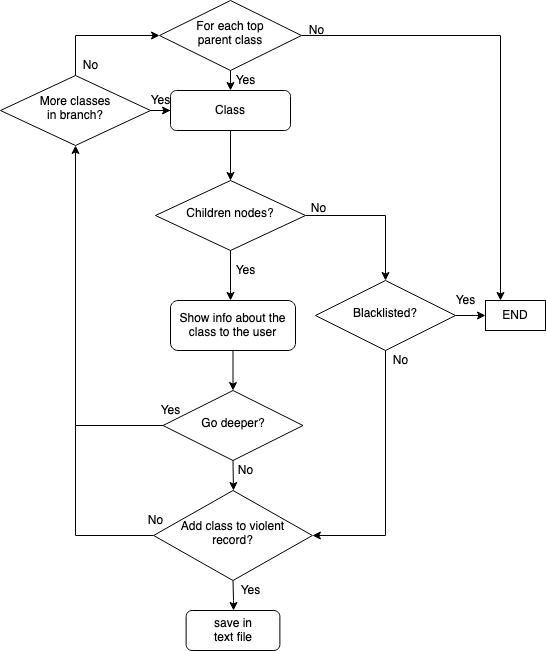
\includegraphics[scale=0.4]{select-vio-cls}
		\caption{Flowchart about selecting violent classes}
		\label{fig:mesh3}
	\end{wrapfigure}
	
	
	Let's say we begin from the class "Human sounds" that is the top level of all sounds emitted by humans contained in the dataset. The system will ask the user if she wants to advance in that direction, i.e., to go across the branches that belong to that part of the tree. If the answer is positive, it would go for the next class, that in this case it would be "Human Speech". It will advance this way until there were no children nodes in the actual class. When this happens, the user will be asked to add the label to the record of \textit{violent classes}, that will be saved in a text file so they can be read by other parts of the model further on. If the user does not want to go deeper, she will be asked to add the current class to the record. If the answer is "No", then they system will jump to the next sibling category. The corresponding flowchart is shown in figure \ref{fig:mesh3}.
	
	This way of flowing through the different classes allows to skip those parts that are not related to our problem. For example, as we can see in figure \ref{fig:mesh1}, one of the top parent labels is "Natural sounds", that relates to sounds from weather phenomena. In most of the cases, these classes will not be selected so the whole branch can be skipped. 

\subsubsection{Downloading videos}

	The following step consists in achieving audio files that belong to the chosen labels. For this purpose, we have made use of the \acrshort{csv} files that were explained in subsection \ref{subsection:data-access}. For each included video, we took its ID and build the corresponding YouTube \acrshort{url}. Once downloaded, we trimmed the file considering the onset and offset and, finally, converted it to audio format (\acrshort{wav}). In our script, we can pass as a parameter the identifier of the desired classes in comma-separated format and either the number of videos per class for a balanced set or a total number of downloads for an unbalanced set. However, there might be some errors when obtaining all the data: the two most common cases are due to lack of enough videos of the desired type in the dataset or because the video is not available anymore on YouTube. When this happens, a message is shown to the user.
	
	It it also worth mentioning that throughout the developing of this downloading task, a script has been coded to achieve the whole dataset in both formats, video and audio, for future works. We are not going to specify anything else since this feature was not finally used.

\subsection{Extracting embeddings}
\label{subsection:extracting-embeddings}

	At this point, all the desired data has been already downloaded to extract the embedded features that will be used to train the model. For this part, we have used the \acrshort{vgg}ish network explained in subsection \ref{subsection:vggish}. Since the audio files duration is usually 10 s, and the embedding extractor gives as a result a vector of size $1 \times 128$ for each second, we will obtain a $10 \times 128$ feature matrix composed by values within the range 0 - 255. Therefore, our input feature matrix will have a size of $(number\ of\ audios) \times 10 \times 128$. The corresponding labels will be stored in a vector of size $(number\ of\ samples)$.
	
	There are some points about the data obtained in this step that should be commented. One of them is about the length of the audio files. As it was previously indicated in \ref{subsection:what-is-audioset}, most of them last 10 s because the creators decided to set this duration for the audio events, but this can change if the video is originally shorter. For these situations, since the model is configured to have an input of $10 \times 128$, the embedding matrix of the shorter clip must be padded with zero-rows to achieve the required dimensions. Even though this does not happen very often, there might be some silent segments that will be labelled with the category of the rest of the audio. A solution for this problem explained later in \ref{section:input-data-preparation} was implemented.
	
	The other case is related to what was explained in \ref{subsection:data-access}. For the recent explanation of how to extract the input features from the audio files we have utilized the first manner of accessing the data, i.e., by reading the \acrshort{csv} files with the videos information before downloading. There is a second option of using the already extracted embedding features. However, these do not look exactly the same when comparing them to the ones obtained by running the \acrshort{vgg}ish with the downloaded videos. This difference is because the implementation of the given code differs from their internal production system in computing issues such as underlying libraries in the installation of \acrshort{vgg}ish and hardware equipment. In spite of this, the result in classification tasks are expected to be equivalent. In order to prove this assumption, we decided to try a small system with both kinds of data. The reason for this check is that although, for this work, the development of the methodologies could be made by using the first and faster manner of accessing the data, for the real implementation in the pendant device within the EMPATIA project (out of our scope) only the second way will be feasible.

\subsection{Assessing the differences between the two types of data access}
\label{subsection:exploring-differences-between-two-types-of-data-access}

	In order to check what is explained above in \ref{subsection:extracting-embeddings}, we have decided to run a little experiment in which a toy classification is performed. Also, we wanted to visualize the different features to check if we could appreciate common patterns by using the \acrfull{tsne} algorithm, which will be explained later in this section.

	Our first step consisted in determining a subset extracted from the original dataset. We thought about choosing for this small application a set composed by three classes that could be considered violent and other three that were non-violent. Apart from this, we paid attention to the number of samples per category to pick some classes over others. Finally, we ended up picking up the labels detailed in table \ref{table:4} and a number of 80 samples for each of them, which led us to a total of 480.
	
	% Table for chosen classes
	\begin{table}[h]
		\begin{center}
			\begin{tabular}{||m{7em} | m{23em} ||}
				\hline
				\textbf{Class} & \textbf{Description} \\
				\hline\hline
				Screaming & A sharp, high-pitched human vocalization; often an instinctive action indicating fear, pain, surprise, joy, anger, etc. Verbal content is absent or overwhelmed, unlike Shout and Yell. \\
				\hline
				Crying, sobbing & Sound associated with the shedding of tears in response to an emotional state, arising from slow but erratic inhalation, occasional instances of breath holding and muscular tremor. \\
				\hline
				Gunshot, gunfire & The sound of the discharge of a firearm, or multiple such discharges. \\
				\hline
				Animal & All sound produced by the bodies and actions of non-human animals. \\
				\hline
				Engine & The sound of a machine designed to produce mechanical energy. Combustion engines burn a fuel to create heat, which then creates a force. Electric motors convert electrical energy into mechanical motion. Other classes of engines include pneumatic motors and clockwork motors. \\
				\hline
				Printer & Sounds of a computer peripheral which makes a persistent human readable representation of graphics or text on paper or similar physical media. \\
				\hline
			\end{tabular}
		\end{center}
		\caption{Chosen classes for a small classification. \textit{Screaming}, \textit{Crying, sobbing} and \textit{Gunshot, gunfire} are considered as the violent ones.}
		\label{table:4}
	\end{table}
	
	For the classification task, we decided to create a small \acrshort{cnn} composed by few layers. Since our input data are matrices of shape $10 \times 128$, these were treated as images so the model was built with layers that perform spatial convolution \cite{Levoy2012}. The architecture is detailed in figure \ref{fig:mesh5}. We used a small kernel size of $3 \times 3$, zero padding so as not to change the shape of the output and a activation of function \acrshort{relu}. Two dense\footnote{Dense is a also a common form to refer to \acrlong{fc} layers. Since each neuron is fed with an input from all the neurons in the previous layer we can say that they are densely connected \cite{Rampurawala2019}} layers are added at the end, first one with also \acrshort{relu} as activation function and the second one with \textit{softmax} to perform the classification, and as many filters as the number of classes.
	
	In order to measure the results, since our subset is balanced, we could have evaluated our model by computing the accuracy and the confusion matrix. More information about these metrics can be found in the appendix \ref{appendix:metrics}. In figure \ref{fig:mesh7}, the four confusion matrices corresponding to the training and test phases for both types of data are shown. Also, in table \ref{table:5}, it is included the accuracy for each case. The results are more accurate when training with the embeddings extracted directly from the audio files we downloaded. When obtaining them from the \acrlong{tf} files, they value of the metrics indicate a worse performance. However, we opted for this second manner because the performance difference is not too big and it requires  much less computational cost and time loss.
	
	% Four confussion matrices
	\begin{figure}[htb]
		% Whole figure
		\captionsetup{justification=centering}
		\begin{subfigure}[b]{\textwidth}
			% Start with figure wav
			\centering
			\captionsetup{justification=centering}
			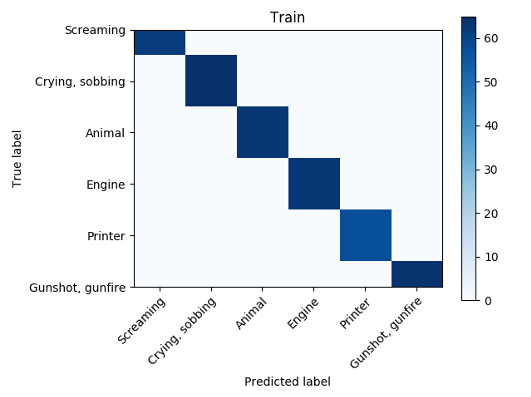
\includegraphics[width=0.5\linewidth]{wav_train}%
			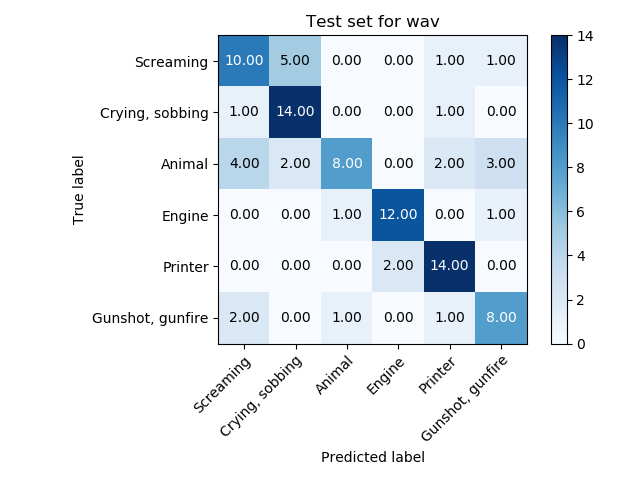
\includegraphics[width=0.5\linewidth]{wav_test}
			\subcaption{Confusion matrices when embeddings are extracted from audio files}
		\end{subfigure}
		\vskip\baselineskip
		% Start with figure tfrecord
		\begin{subfigure}[b]{\textwidth}
			\centering
			\captionsetup{justification=centering}
			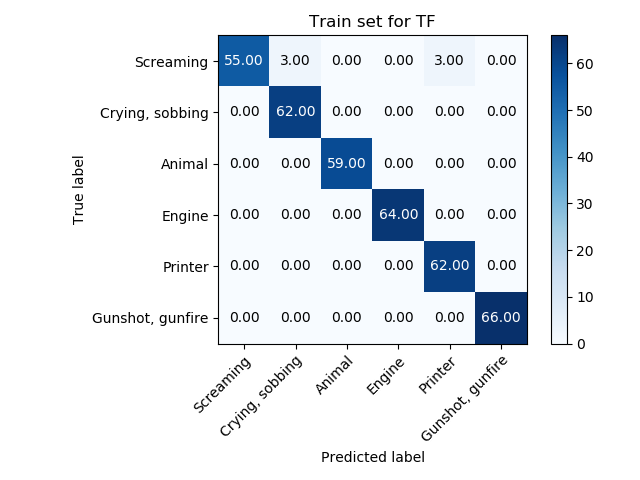
\includegraphics[width=0.5\linewidth]{tfrecord_train}%
			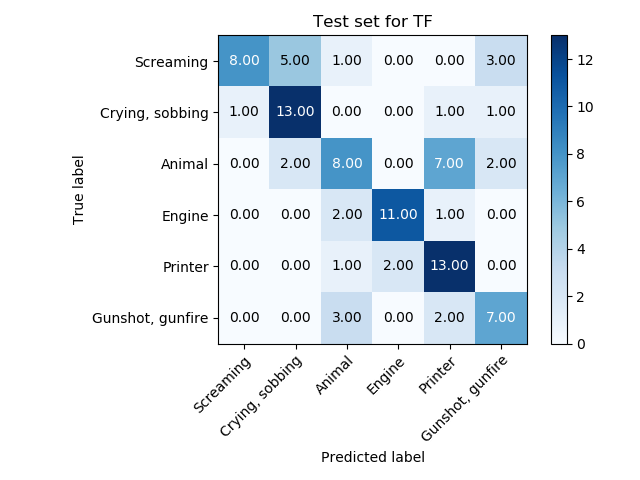
\includegraphics[width=0.5\linewidth]{tfrecord_test}
			\subcaption{Confusion matrices when embeddings are taken from .\textit{tfrecord} files}
		\end{subfigure}
		\caption{Confusion matrices}
		\label{fig:mesh7}
	\end{figure}
	
	% Accuracy values train and test
	\begin{table}[h]
		\begin{center}
			\centering
			\begin{tabular}{|| m{7em} | m{7em} | m{7em} ||}
				\hline
				format / subset & \textbf{Train} & \textbf{Test} \\
				\hline\hline
				\textbf{Audio file} & 0.98 & 0.63 \\
				\hline
				\textbf{.\textit{tfrecord}} & 1.0 & 0.72 \\
				\hline
			\end{tabular}
		\end{center}
		\caption{Accuracy values for audio and .\textit{tfrecord} files}
		\label{table:5}
	\end{table}
	
			% Architecture of model of user interact system
	\begin{wrapfigure}[15]{R}{0.4\textwidth}
		\centering
		\captionsetup{justification=centering}
		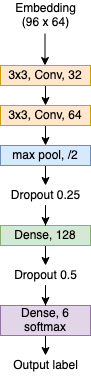
\includegraphics[scale=0.6]{try-wav-tf}
		\caption{Architecture to see how the different embeddings work}
		\label{fig:mesh5}
	\end{wrapfigure}
	
	For the training phases, it can be appreciated that there may be an overfitting since the accuracy is perfect. This means that the \acrshort{nn} stop improving its capacity of learning how to solve the problem in a certain moment of the training task. Instead, it does learn some behaviour pattern that the training data follows. This impacts negatively in the model since the new data that the system will have to learn from will look different and will not follow these same rules \cite{Jabbar2015}. In spite of this result, we did not give it so much importance since we just wanted to do a quick check of the similarity between the two types of data which can be appreciated due to the similarity of both metrics results.
	
\subsubsection{Dimensionality reduction for visualization}
\label{subsection:dimensionality-reduction-for-visualization}

	Apart from the classification exercise, we wanted to see if by plotting the data samples we were able to identify or appreciate some common patterns. In our problem, each of our samples is characterized by a matrix of features with 128 columns, which means that we were working with data belonging to a high-dimensional space. Visualizing this type of data has always been a case of study for many different fields. Plenty of methods have been published so as to find a solution for this task. Some of the most accepted consist on reducing the dimensionality of the data so this can be transformed from the high-dimensional space to a lower one and can be visualize in a common scatter plot of 2D or 3D. These techniques rely on the idea that within a multivariate sample denoted as $x_i = [x_{i1},..., x_{in}]^T$ and considered to be a point that corresponds to a $n-dimensionality$ space, a $d-dimensionality$ space can be found, so that $d < n$. %, in which the data \doubt{is included}. 
	If this is possible, then the observations can be transformed to this lower dimensional space $d$ without any loses \cite{Kaski2011}. 
	
	One of the most common and well-known dimensionality reduction methods is the one known as \acrfull{pca}. This follows the idea previously explained. It specifically aims at extracting the \textit{important} information from the original data and transform them into a set formed by orthogonal variables which are actually known as principal components. This is done by multiplying the matrix data $X$ by a projection matrix $Q$ that contains the coefficients of the linear combinations that allow the conversion. The projections must be orthogonal to each other and they represent the data maximum variance in descending order, being the first component the one with largest variance \cite{Abdi2010}. In fact, each of the projections correspond to an eigenvector in descending order following the value of the eigenvalue. So, the first component will be the eigenvector with the highest eigenvalue. It has been proved to be one of the most appropriated options in dimensionality reduction nowadays. Its use is completely accepted and it is implemented in many famous software libraries. However, it presents some limitations. One of them consists on just considering linear combinations of the original data. When the relation is non-linear, a dimensionality reduction with this technique may result in a loss of information \cite{AmatRodrigo2017}. 
	
	For these cases, other methods have been developed such as \acrfull{tsne}. This algorithm appears as an extension of the previously published \acrfull{sne} \cite{Hinton2003}. Both are based on the same idea of a new way of measuring the similarity between samples. Instead of comparing two observations, let's call them $x_i$ and $y_j$, by computing the euclidean between them, this is done by calculating the conditional probability $p_{j|i}$ of $x_j$ being picked as a neighbour of $x_i$ considering that the samples belong to a Gaussian distribution centered at $x_i$. This depends on how far the samples are from each other, i.e., it is high when they are close and minimum when there are totally separated \cite{VanDerMaaten2008}. Apart from this, two analogous observations are created in the subspace of lower-dimensionality, $y_i$ and $y_j$, and conditional probability $q_{j|i}$ is computed in this situation. It is important that, for $y_i$ and $y_j$ to be faithful representations of $x_i$ and $x_j$, both conditional probabilities must be equal.
	
	In order to calculate the probabilities, a crucial factor is the variance of the Gaussian distribution. There is not a unique valid choice for this parameter, so \acrshort{tsne} performs a binary search so as to find the optimal one \cite{AmatRodrigo2017}. This is also influenced by what is called the perplexity. This can be defined as an assumption of the number of adjacent neighbours for each point. It is a value that is fixed by the user, but it usually belongs to a range from 5 to 50 \cite{VanDerMaaten2008}. 
	
	There are several considerations that should be known before looking at a representation of data from this algorithm \cite{Wattenberg2016}. Actually, it is not an easy task to understand this kind of plots, since the distance between points in the new subspace are not related to the real euclidean distance, which has been denoted as "The Crowding Problem" \cite{VanDerMaaten2008}. This means that the groups cannot be interpreted as real collections of data in the original dimension. However, in order not to misunderstand the data distribution, a couple of visualizations varying the parameters usually tends to be done so that the conclusions can be based on more than one result. In figures \ref{fig:mesh8} and \ref{fig:mesh52}, we show ten \acrshort{tsne} outputs, five for each type of data for diverse values of perplexity from 2 to 50, respectively.
	
	% Four confussion matrices
	\begin{figure}[H]
		% Whole figure
		\captionsetup{justification=centering}
		\begin{subfigure}[b]{\textwidth}
			% Start with figure wav
			\centering
			\captionsetup{justification=centering}
			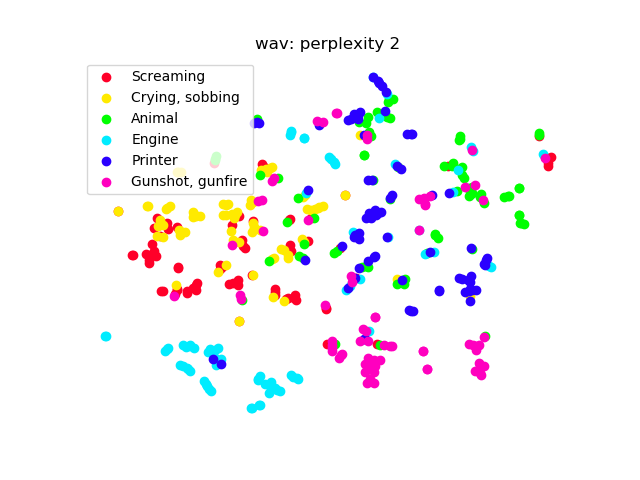
\includegraphics[width=0.5\linewidth]{wav-perp-2}%
			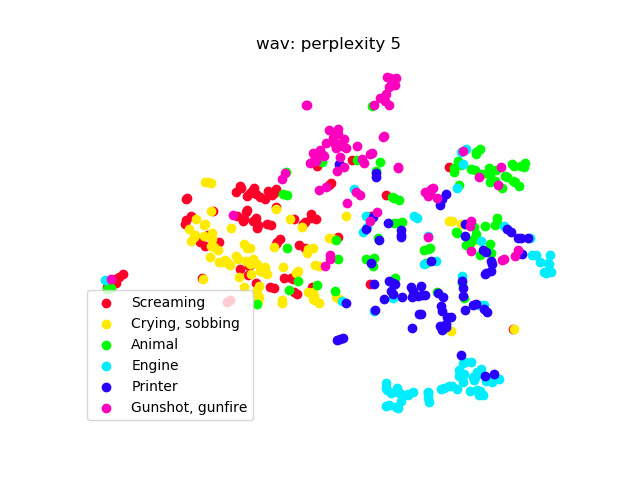
\includegraphics[width=0.5\linewidth]{wav-perp-5}%
		\end{subfigure}
		\vskip\baselineskip
		% Start with figure tfrecord
		\begin{subfigure}[b]{\textwidth}
			\centering
			\captionsetup{justification=centering}
			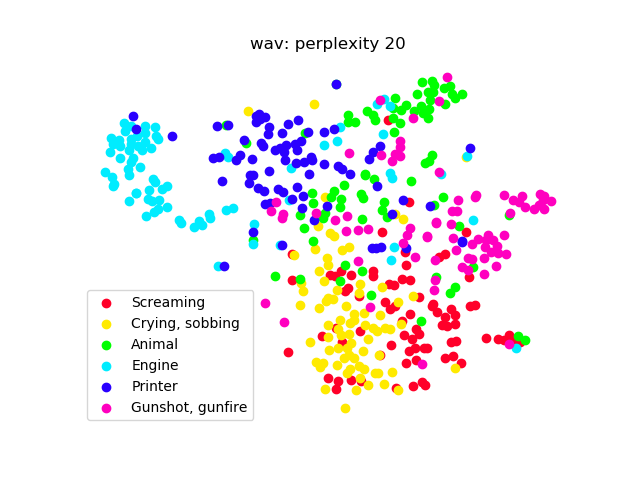
\includegraphics[width=0.5\linewidth]{wav-perp-20}%
			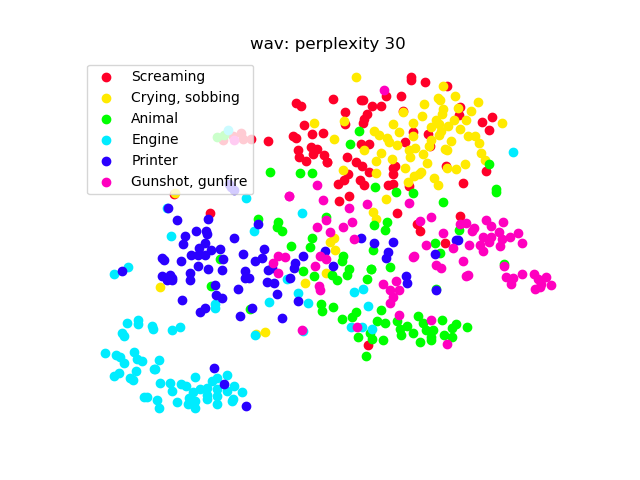
\includegraphics[width=0.5\linewidth]{wav-perp-30}%
		\end{subfigure}
		% 
		\begin{subfigure}[b]{\textwidth}
			\centering
			\captionsetup{justification=centering}
			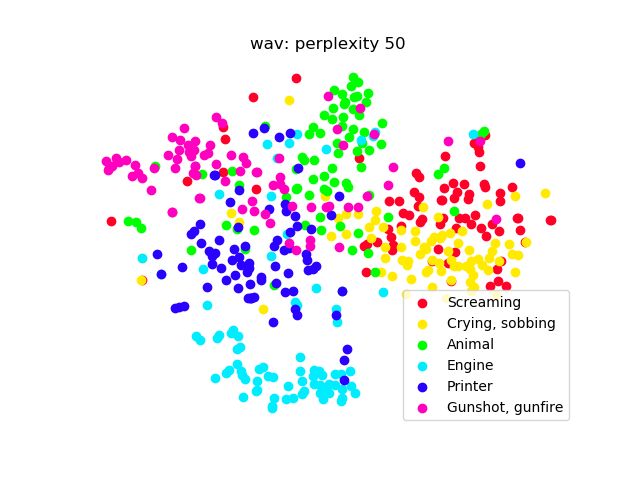
\includegraphics[width=0.5\linewidth]{wav-perp-50}
		\end{subfigure}
		\caption{t-SNE results for wav format with a legend that shows the labels of the corresponding samples in the original 128D space}
		\label{fig:mesh8}
	\end{figure}
	
	\todo{CPM: aumentar las figuras para que se puedan leer las leyendas.}
	
	The selection of the perplexity value depends on the number of observations per class \cite{Wattenberg2016}. Since our subset has 80 samples for each category, we can consider that a proper value is 20 or 30. As we can see, a boundary cannot be extracted among the different labels, but we can see some grouping patterns in the data that correspond to the original labelling and helps us to confirm the similarity of the two different given types. It is true that this method should never be used as an algorithm for clustering itself, but it is a good resource as a backing strategy to other results, as in this case. 
	
	% Four confussion matrices
	\begin{figure}[H]
		% Whole figure
		\captionsetup{justification=centering}
		\begin{subfigure}[b]{\textwidth}
			% Start with figure wav
			\centering
			\captionsetup{justification=centering}
			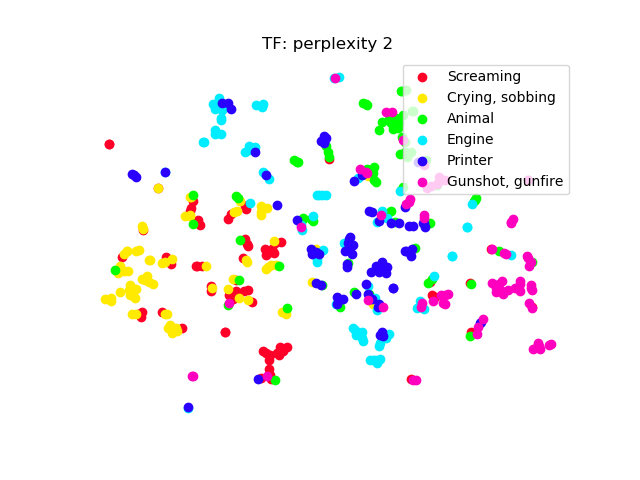
\includegraphics[width=0.5\linewidth]{TF-perp-2}%
			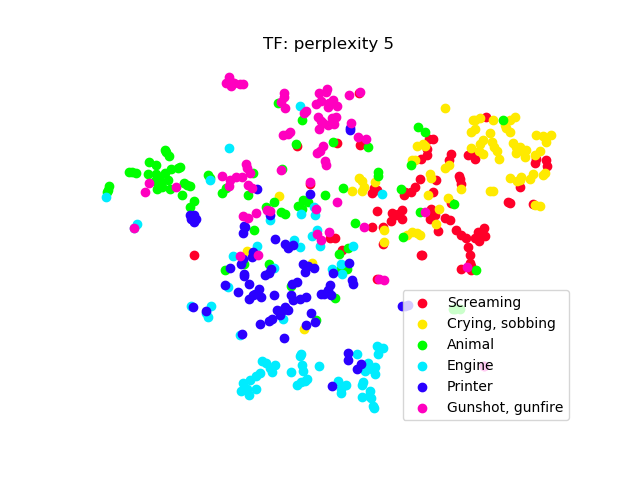
\includegraphics[width=0.5\linewidth]{TF-perp-5}%
		\end{subfigure}
		\vskip\baselineskip
		% Start with figure tfrecord
		\begin{subfigure}[b]{\textwidth}
			\centering
			\captionsetup{justification=centering}
			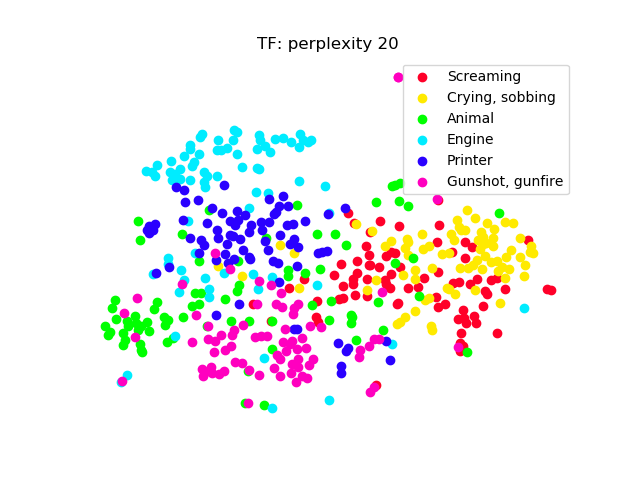
\includegraphics[width=0.5\linewidth]{TF-perp-20}%
			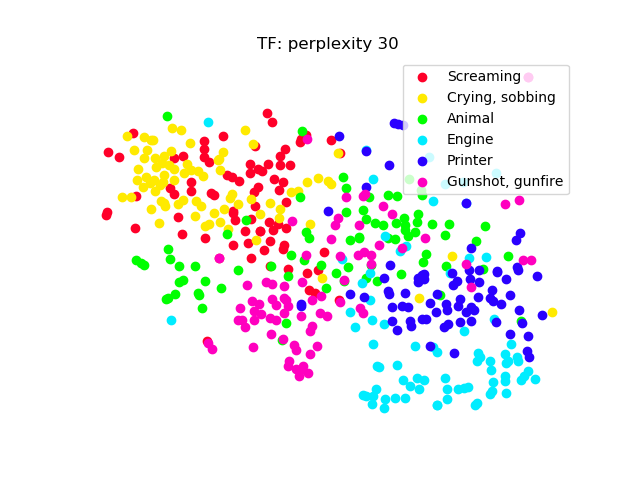
\includegraphics[width=0.5\linewidth]{TF-perp-30}%
		\end{subfigure}
		% 
		\begin{subfigure}[b]{\textwidth}
			\centering
			\captionsetup{justification=centering}
			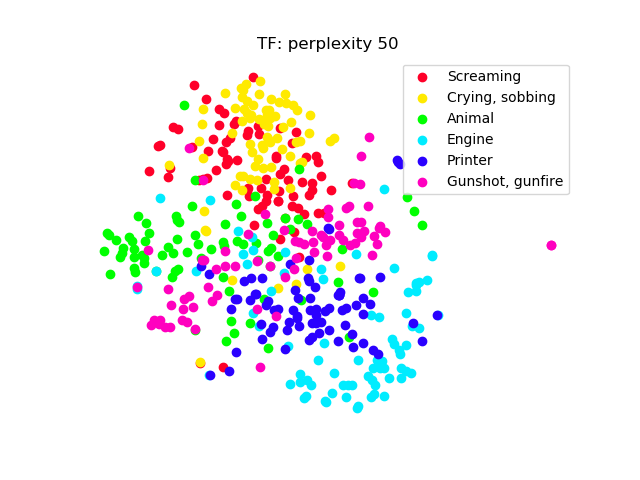
\includegraphics[width=0.5\linewidth]{TF-perp-50}
		\end{subfigure}
		\caption{t-SNE results for .\textit{tfrecord} format with a legend that shows the labels of the corresponding samples in the original 128D space}
		\label{fig:mesh}
	\end{figure}

\section{Methodology}
\label{section:models}
	
	\todo{Debería poner ejemplos de aplicación al audio como hice en las CNNs o simplemente dejarlo así y ya tratarlo como una parte del estado del arte de related work}
	
% Explain the methods used:
% 1) Data augmentation and SMOTE
% 2) SVM 
% 4) CNN
% 5) LSTM

% !TeX spellcheck = en_GB

\subsection{\acrfull{smote}}
\label{subsection:smote}

	\acrshort{smote} consists of an over-sampling method whose function is to generate synthetic samples in order to populate the minority class in a classification problem by making use of the proper observations that are already contained in the data \cite{Chawla2002}. 
	
	Essentially, this technique works by choosing samples from the minority class that are represented in the features space, placing a line between two of these samples and then select a point inside the line at a random position. First, an arbitrary sample is picked from the minority class and then a number of \textit{k} closest neighbours in the feature space are selected from the same class. One of the neighbours are randomly chosen and a synthetic sample is generated between these two \cite{Browniee2020}. The number of neighbours \textit{k} can vary depending on the amount of over-sampling needed. The value proposed in the publication paper is \textit{k = 5} \cite{Chawla2002}. 
	
	For the generation of the synthetic samples, the distance between the feature vector first arbitrarily selected and one of the nearest neighbours is computed. Then, the resulting value is scaled by multiplying it by a random number that lies in the uniform distribution $U(0,1)$. Finally, this new sample, \textit{S}, is added to the initial feature vector and placed in between these two observations in the feature space \cite{Chawla2002}. \textit{S} can be defined as follows:
	\[S = x + u\cdot(x^{R} - x) \]
	where \textit{x} is the arbitrary selected sample the first time, \textit{u} is the random value from $U(0,1)$ and \textit{x\textsuperscript{R}} is the closest neighbour \cite{Blagus2013}. In figure \ref{fig:mesh47}, it shown a graphical representation of the algorithm. In this case, \textit{X} is the original sample for which the closest neighbours are represented as $X_{i}$, $i=1,2,3,4,5$. The generated samples are $Y_{1}$ and $Y_{2}$ that are place in the line segments.
	
	\begin{figure}
		\centering
		\captionsetup{justification=centering}
		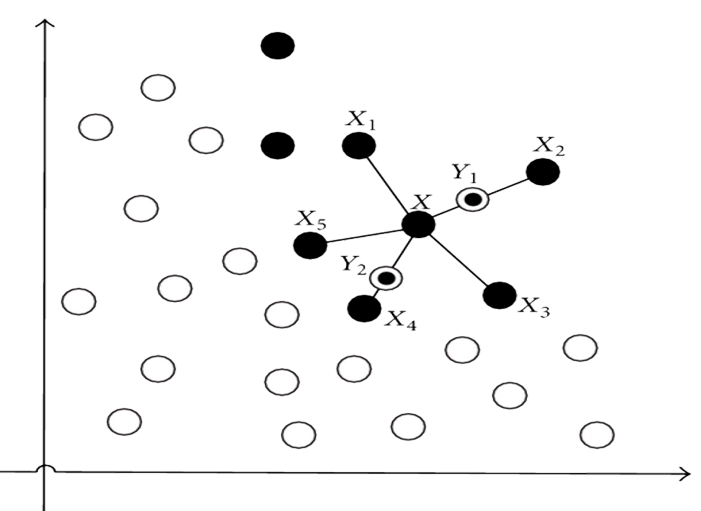
\includegraphics[scale=0.3]{SMOTE}
		\caption{SMOTE algorithm \cite{Xie2015}}
		\label{fig:mesh47}
	\end{figure}

	The common way of applying this technique is in the train set before performing the fit of the model. Usually, an under sampling is performed in the most populated classes and, then, the data augmentation is done for the minority ones \cite{Browniee2020}. Our implementation follows this rule and it is explained in section \ref{section:input-data-preparation}.
	
	 

% !TeX spellcheck = en_GB

\subsection{\acrfull{svm}}
\label{subsection:svm}

	\todo{Adapt...}
	Considering instances of data with their respective ground-truth labels, this classifier finds the frontier defined as a hyperplane that maximizes the distance between the two observations closest to each other that belong to different classes and are more likely to be misclassified. These two points are called support vectors \cite{Fu2011}. This type of method is characterized for being a binary classifier. However, its implementation has been transported to multiclass problems by combining various \acrshort{svm}s in order to stablish a decision criterion so the whole system can chose among $Q$ categories. This can be done by following either one-versus-all or one-versus-one approach. The former addresses the problem training $Q$ classifiers so as to differentiate between data from one class and data from the other $Q-1$ classes. The latter treats the problem by training $Q(Q-1)/2$ \acrshort{svm}s to distinguish among all possible combinations of categories. In any of the approaches, the classification of a certain observation is performed by computing the distance between the sample data and the hyperplane that defines the frontier \cite{Barchiesi2015}. The one-versus-one is the one implemented by \acrfull{svc} from Scikit-learn library and is the one we will use in one of the experiments explained in section \ref{}. In figure \ref{fig:mesh10} it is shown a representation of the decision boundaries that could designed by other type of methods against the hyperplane a \acrshort{svm} classifier would draw.
	
	\begin{figure}[h]
		\centering
		\captionsetup{justification=centering}
		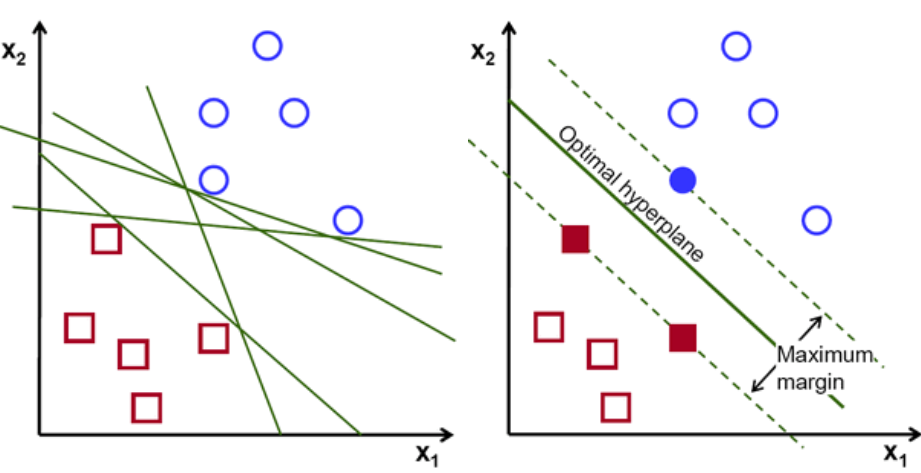
\includegraphics[scale=0.2]{svm}
		\caption{Visualization of a hyperplane set by \acrshort{svm} and other decision boundaries \cite{Drakos2018}}
		\label{fig:mesh10}
	\end{figure}
	
\todo{Add requisites for sklearn algorithm and details about implementation in our model}
\todo{Include definition of kernel and cases}

% !TeX spellcheck = en_GB

\subsection{\acrlong{rnn} and \acrlong{lstm}}

	Human learning does not happen at each moment independently in the sense that every time something new is learned, it depends on the previous knowledge in order to interpret it. This can also be explained by saying that our understanding is persistence.
	
	Traditionally, \acrlong{ann} are not able to act in this way. They \doubt{cannot use the time} as a property to infer conclusions or predictions from the previous instances that belong to a sequence of data. To address this task \acrfull{rnn} have been developed, so they can take information and make it persistent. In figure \ref{fig:mesh39}, it is shown a block of a \acrshort{rnn} in which the network, \textit{A}, is fed with an input \textit{x\textsubscript{t}} that is actually a sequence of data. The output is the value \textit{h\textsubscript{t}}. An inner loop takes the information from the outcome and pass to the input for the next learning step. This can be easily seen in the unrolled part of the right, how the information flows from one element to the next one \cite{Olah2015}. 
	
	\begin{figure}[h]
		\centering
		\captionsetup{justification=centering}
		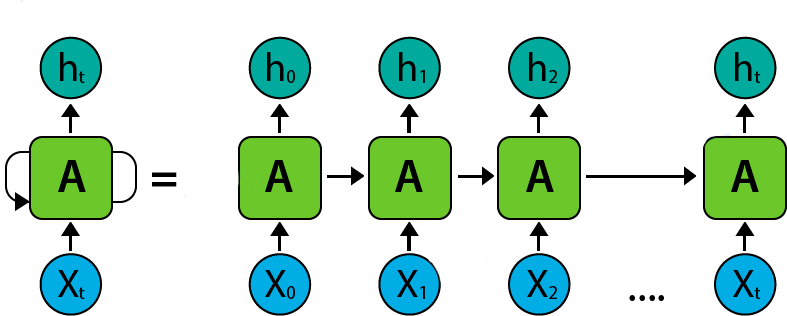
\includegraphics[scale=0.35]{rnn}
		\caption{Scheme or a recurrent neural network about how the loop works }
		\label{fig:mesh39}
	\end{figure}

	This type of networks has became the standard when dealing with sequential data. They have been applied in many tasks, such as language modelling, speech recognition, translation, etc. However, the most simple approach present a problem when the information that must be considering when long-term dependencies. For example, if the task consists of predicting a new instance based on the previous ones in a not really long sequence in which the dependency resides on close instances, normal \acrshort{rnn} can be used and work in the way explained above. When the distance inside the sequence between the predicted element and the ones with the important information that this new one depends on is too large, the network cannot learn this connection \cite{Olah2015}. 
	
	\begin{figure}[h]
		\centering
		\captionsetup{justification=centering}
		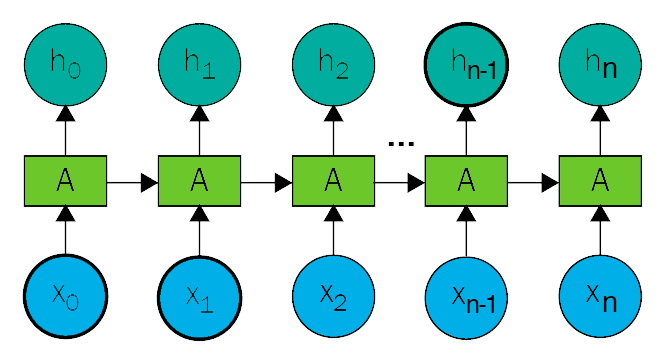
\includegraphics[scale=0.35]{long-term-dependencies}
		\caption{Example of long-term dependencies situation. If the predicted output h\textsubscript{n-1} depends on x\textsubscript{0} and x\textsubscript{1}, the vanishing gradient problem may appear.}
		\label{fig:mesh40}
	\end{figure}
	
	This happens due to the value of the gradients becomes very small during the backpropagation in the learning process. Once the loss function for the new predicted output is calculated, this must be propagated through the rest of the network in order to update the weights. In a typical neural network model, \doubt{the neurons that get updated are those from the hidden layer directly previous to the output one}, but, since the data is a sequence, the neurons from all the earlier layers must be updated as well. The actual problem appears when renovating the value of the weights through time, i.e. updating the weights used to connect the hidden layers in the unrolled temporal loop. So, if the value of the gradient becomes very small the updating process start to be null when finding the new values of the weights and the model stop learning. This is known as the vanishing gradient problem \cite{SuperDataScienceTeam2018}.
	
	As a solution, a new type of \acrshort{rnn} was developed and named as \acrfull{lstm} networks. These can be defined as a recurrent network that can learn long-term dependencies, so the vanishing gradient problem is not an issue for these models. Nowadays, they are widely used in several fields, since they can remember information along long periods \cite{Olah2015}. The main structure along is the same shown above in figure \ref{fig:mesh39}. The difference from the way of working in a common \acrshort{rnn} is the inner architecture in the neural network. In \acrshort{lstm}, the \textit{A} modules are defined as shown in figure \ref{fig:mesh41}. The notation used is as follows: the rectangles denotes a neural network layer, the circle shapes refer to point-wise operations and the arrows means vector transferring.
	
	\begin{figure}
		\centering
		\captionsetup{justification=centering}
		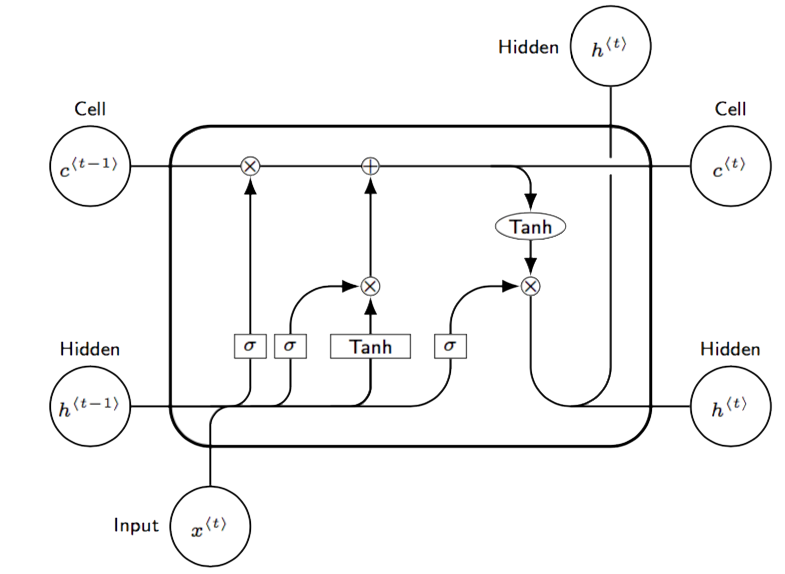
\includegraphics[scale=0.29]{lstm-module}
		\caption{LSTM module with the representation of the different operations that take place inside of it}
		\label{fig:mesh41}
	\end{figure}

	The main concept of a \acrshort{lstm} network resides on its cell state and the different gates. The cell state, represented in the diagram by the upper arrow, is the one in charge of transferring information all the way through the chain of modules. It can be thought as the memory of the whole network. Its objective is to just carry information considered relevant for the model. This way is how the \acrshort{lstm} brings the information from the first layers to the last ones without suffering the vanishing gradient problem. The content of the cell state is modified by the point-wise operations that acts by following the gates criteria. These are in fact neural networks that has the goal of deciding which information can be treated as relevant and so added to cell state. This process can be understood as a learning/forgetting stage \cite{Nguyen2018}. 
	
	In order to understanding how this process works, we are going the interaction of the different gates in the learning stage.

	\begin{wrapfigure}{l}{0.26\textwidth}
		\centering
		\captionsetup{justification=centering}
		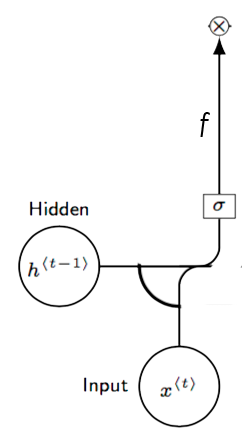
\includegraphics[scale=0.25]{lstm-forget-gate}
		\caption{Step 1. Forget gate}
		\label{fig:mesh42}
	\end{wrapfigure}

	The first step is performed by what is called the \textit{forget gate} layer. It must decide which information must be included in the cell state that travels through the time chain. This is way the layer contains a sigmoid function that outputs values between  0 and 1, in which  0 means dropping the information in the previous cell state and 1 implies to keep it. As shown in figure \ref{fig:mesh42}, this is done by paying attention to the hidden state which is the output of the previous module, \textit{h\textsuperscript{<t-1>}}, and the input of the current one, \textit{x\textsuperscript{<t>}} \cite{Nguyen2018}. The resulting function $f$ is defined as follows, where $W_{f}$ are the weights of the \acrshort{rnn} and $b_{f}$ the bias.
	\[
	\ f = \sigma(W_{f}[h^{t-1}, x^{t}] + b_{f})
	\]
	
	\begin{wrapfigure}{r}{0.3\textwidth}
		\centering
		\captionsetup{justification=centering}
		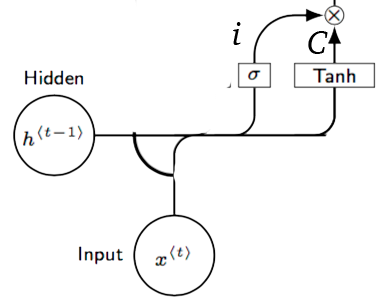
\includegraphics[scale=0.27]{lstm-input-gate}
		\caption{Step 2. Input gate}
		\label{fig:mesh43}
	\end{wrapfigure}
	
	Next, the decision about what information from the current input \textit{x\textsuperscript{<t>}} must be taken to the cell state is performed. The gate that computes this operation receives the name of \textit{input gate}. This part can be divided into two different steps. First, the previous hidden state,\textit{x\textsuperscript{<t-1>}} ,and the current input feed a \acrshort{rnn} with a sigmoid for the activation function, which takes the decision of \doubt{which values must be updated} by converting them into a range limited by 0 and 1. This result denotes the importance of the value, being 0 non-important and 1, important. Then, also \textit{h\textsuperscript{<t-1>}} and \textit{x\textsuperscript{<t>}} are used as input for the \acrshort{tanh} layer so the values are mapped between -1 and 1. This last activation function is included in order to \doubt{avoid the vanishing gradient problem previously mentioned, since a function whose second derivative takes more time to tend to zero is needed}. Finally, both outputs are multiplied before the updating process in the cell state \cite{Nguyen2018}. The equations for the output of each \acrshort{rnn} module are included below, where $W$ and $b$ denotes the weights and bias for each layer \cite{Olah2015}.
	\[ i = \sigma(W_{i}[h^{t-1}, x^{t}] + b_{i}) \]
	\[ C = \tanh(W_{C}[h^{t-1}, x^{t}] + b_{C}) \]
	
	In the step 3, the output of the multiplication from the input gate layer and the output $f$ of the sigmoid function from the forget gate, modify the old cell state from the previous module, \textit{c\textsuperscript{<t-1>}}, so it can be updated. For the outcome of the step 1, a point-wise multiplication is performed, $f * C^{<t-1>}$. Then, to the output of this operation is added the resulting product of the input gate, $i * C$. This two operations can be translated as a forgetting and a learning stage. First, the values the forget gate decided to remove from the cell state are actually forgotten. Then, it must learn the new values belonging to the current input also weighted by their importance, what denotes how much the state values are going to be updated \cite{Olah2015}. The new cell state expression $c^{t}$ is included below and the process is shown in figure \ref{fig:mesh44}.
	
	\begin{wrapfigure}{l}{0.4\textwidth}
		\centering
		\captionsetup{justification=centering}
		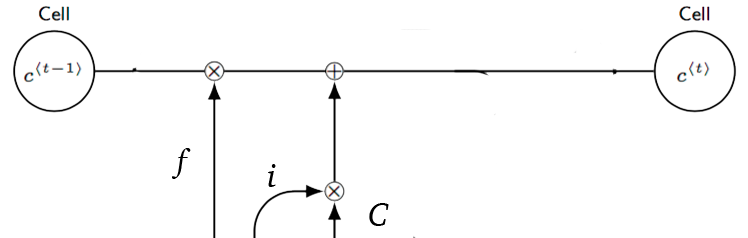
\includegraphics[width=\linewidth]{lstm-cell-state}
		\vspace{-10pt}
		\caption{Step 3. Update cell state}
		\label{fig:mesh44}
	\end{wrapfigure}
	
	
	\[c^{<t>} = f * C^{<t-1>} + i * C\]
	
				
	Finally, the last step of the module corresponds to the \textit{output gate}. This has the function of deciding how the next hidden state is going to be like. First, \textit{x\textsuperscript{<t>}} and \textit{h\textsuperscript{<t-1>}} are used as input for a layer with a sigmoid activation function and the output $o$ is obtained. Also, the cell state \textit{c\textsuperscript{<t>}} feeds a point-wise \acrshort{tanh} so its values are clipped between -1 and 1. Both outputs are multiplied. The $o$ result decides what values form the current input must be kept in the future hidden state,\textit{h\textsuperscript{<t>}}. The actual output of the module is the hidden state. It also transports the relevant information updated together with the cell state to the next network. The outputs $o$ and $h^{t}$ can be defined as shown below. Also, in figure \ref{fig:mesh45}, the stage of this last part is included.
		
	\begin{figure}{h}
		\centering
		\captionsetup{justification=centering}
		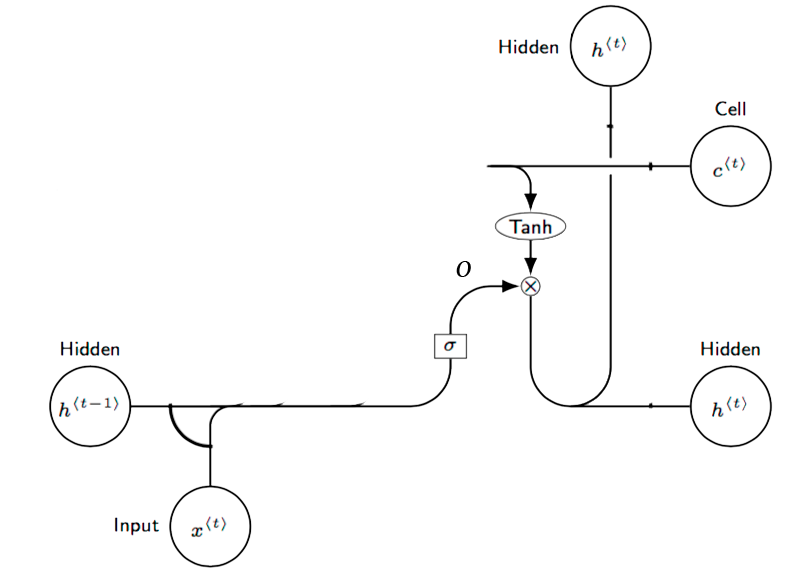
\includegraphics[scale=0.25]{lstm-output-gate}
		\caption{Step 3. Output gate}
		\label{fig:mesh45}
	\end{figure}
	
	\[ o = \sigma(W_{o}[h^{<t-1>, x^{t}}] + b_{o}) \]
	\[ h^{<t>} = o * \tanh(C) \]
	
	
	
	
























\chapter{Experiments}
% !TeX spellcheck = en_GB
\label{chapter:experiments}

	In this chapter we are going to explain the final models we chose for our work and the input data preparation to feed these models with. For the different solutions, we have used the algorithms previously explained in the methodology section \ref{section:methodology}. Below, it is presented a list including the 6 implementations compared:
	
	\begin{itemize}
		\item \acrshort{svm} classifier for multiclass classification
		\item \acrshort{svm} multiclass + \acrshort{svm} for a final binary classification
		\item \acrshort{lstm} for multiclass classification
		\item \acrshort{lstm} multiclass + \acrshort{svm} for a final binary classification
		\item \acrshort{cnn} for multiclass classification
		\item \acrshort{cnn} multiclass + \acrshort{svm} for a final binary classification
	\end{itemize}
	

\section{Input data preparation}
\label{section:input-data-preparation}

	For the proposed experiments, we have decided to build a small dataset with the embeddings extracted form the .\textit{tfrecord} files that belong to 14 classes: half of them \textit{violent} and the other half, \textit{non-violent}. To find these, we first did a run on the simple user-interaction program that is explained in \ref{subsection:violent-classes} as if we were gender-based violence victims. As we said, a total of 28 classes were selected. From this set, we picked 7 as the violent classes. The other 7 were chosen just by looking at the ontology to provide negative classes.
	
	It is important to mention that this collection of data is composed by samples with just one label assigned. As explained before in \ref{section:audioset}, the Audio Set database is highly unbalanced. Some of the most appropriated classes to be considered violence are scarcely populated. When doing the selection of categories, apart from paying attention to the own meaning of the class, we also checked the number of samples. For the non-violent type, this was not a problem, since we took some of the most populated labels. However, in the violent case, we had to deal with the requirement of representing violence and also having enough observations. So, due to these limitations, we could not obtain a naturally balanced set. In table \ref{table:7}, the 14 selected labels are shown. %that were selected divided in violent and non-violent. 
	In figure \ref{fig:mesh14}, a bar plot shows the number of samples obtained per class right after the selection. 
	
	\begin{table}[ht]
		\centering
		\begin{tabular}{|| m{10em} | m{10em} ||}
			\hline
			\textbf{Violent} & \textbf{Non-violent} \\
			\hline\hline
			Baby cry, infant cry & Printer \\
			\hline
			Slap, smack & Music \\
			\hline
			Screaming & Speech \\
			\hline
			Machine gun & Vehicle \\
			\hline
			Breaking & Animal \\
			\hline
			Slam & Dishes, pots, and pans \\
			\hline
			Yell & Wind \\
			\hline
		\end{tabular}
	\caption{Relation of \textit{violent} and \textit{non-violent} selected classes}
	\label{table:7}
	\end{table}
	
	\begin{figure}[t]
		\centering
		\captionsetup{justification=centering}
		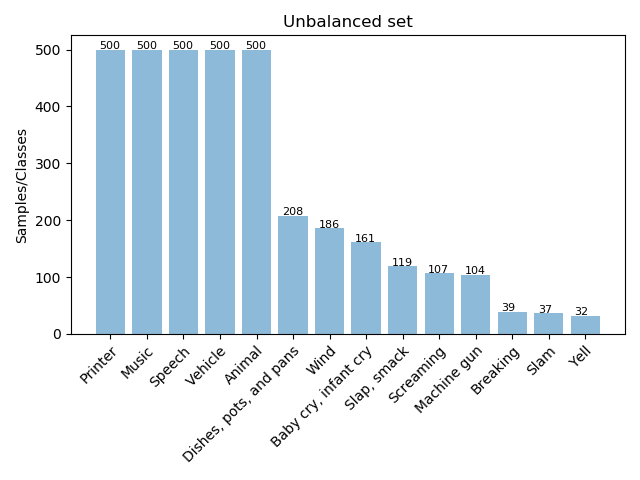
\includegraphics[scale=0.5]{samples-class-experiments}
		\caption{Bar plot that shows the number of samples for each of the selected classes. Clearly, the violent categories are much less populated than the others, that did not have to much any semantic criteria}
		\label{fig:mesh14}
	\end{figure}

	Some initial preprocessing steps were performed before passing the data to the different models. As mentioned in \ref{subsection:extracting-embeddings}, we had to deal with the zero-filling problem, which means that some of the rows of the embeddings matrices are completely zero because the duration of the original video is less than 10s. As a solution, we decided to substitute the zero numbers in all the data with the machine epsilon\footnote{The machine epsilon value is considered the smallest value that satisfies $1 + \epsilon_{match} > 1$. It is the difference between one and the next closest number that is representable as a machine value \cite{Kaw}} value. 
	
	However, in the two models that use \acrshort{svm} for the multiclass classification a different solution was proposed. This algorithm needs the input data matrix to be in the form [$number\ of\ samples\ \times\ number\ of\ features$], which differs from the originally shape of our data, [$number\ of\ samples\ \times\ number\ of\ seconds\ \times\ number\ of\ features$]. For this reason, we decided to reshape our data to the required form which resulted in a matrix of shape [$(number\ of\ samples\ \times\ number\ of\ seconds)\ \times\ number\ of\ features$]. With this conversion, instead of working with full audio instances, the data samples became the seconds of those instances. In order to remove zero data, we first checked the amount of zero-rows in every class. Since it was not a very significant portion of the data, we took them out of the dataset. 
	
	Once we had our data with all non-zero values, we needed to convert the unbalanced set to balanced. First, for the classification task, we divided our data into train, validation and test subsets, using a 20\% for last one. Then, we decided to exclude half of the samples from the most populated classes from the train and validation sets %half of the samples from the most populated classes 
	\footnote{\textit{Speech}, \textit{Music}, \textit{Vehicle} and \textit{Animal}}. In figure \ref{fig:mesh15}, subfigure (a) shows the distribution of data per class in the dataset for the models that use \acrshort{svm} multiclass classifier. In subfigure (b), the distribution for the other four cases is shown. Then, we wanted to generate new data for those with less observations by applying the data augmentation technique \acrshort{smote}, explained in subsection \ref{subsection:smote}, in order to generate samples until equalize the most populated category. Just the train and validation sets were subjected to this conversion process, leaving the test set with the original number of embeddings in their natural a priori state. The final shape of the input data for each of the experiments is shown in table \ref{table:8}.
	
	\begin{figure}[H]
		% Whole figure
		\captionsetup{justification=centering}
		\begin{subfigure}[b]{\textwidth}
			% Start with figure wav
			\centering
			\captionsetup{justification=centering}
			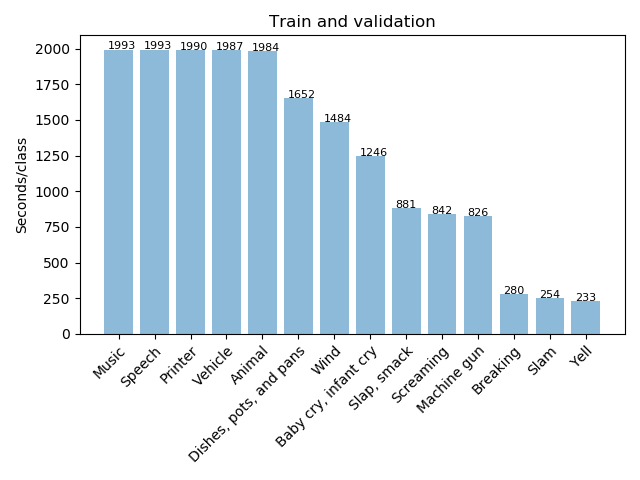
\includegraphics[width=0.5\linewidth]{tr_val_unbal_svm}%
			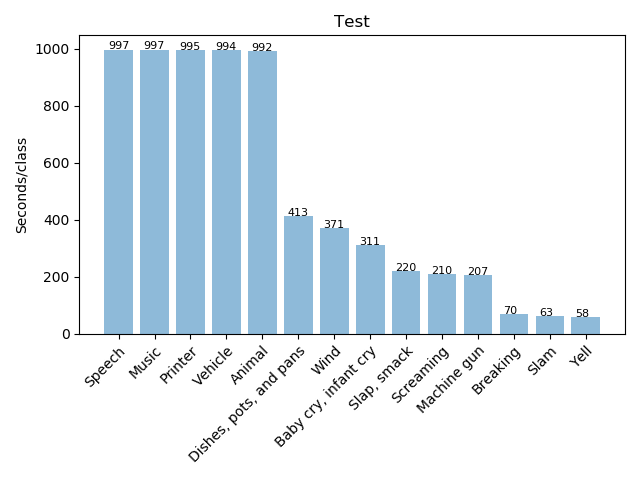
\includegraphics[width=0.5\linewidth]{tst_unbal_svm}
			\subcaption{This are the resulting subsets after downsampling the most populated classes and removing the zero-rows for the experiments that involve an SVM classifier}
		\end{subfigure}
		\vskip\baselineskip
		% Start with figure tfrecord
		\begin{subfigure}[b]{\textwidth}
			\centering
			\captionsetup{justification=centering}
			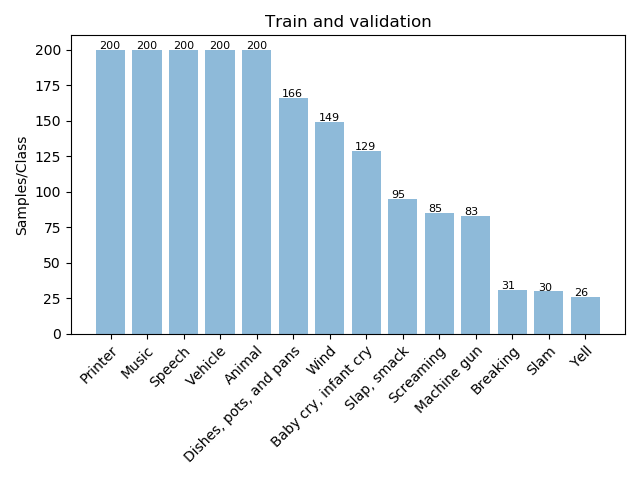
\includegraphics[width=0.5\linewidth]{tr_val_unbal}%
			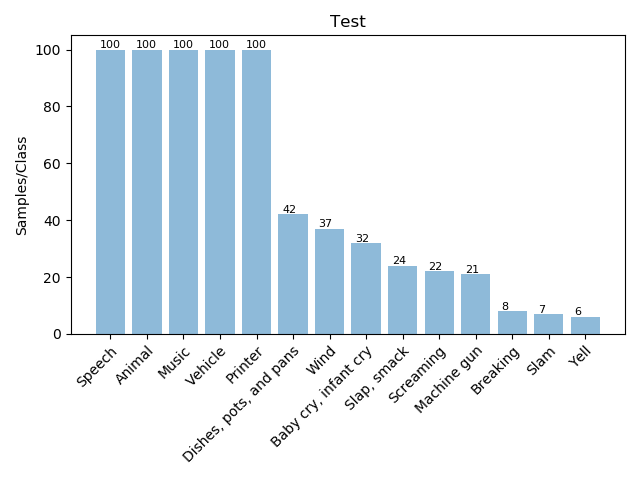
\includegraphics[width=0.5\linewidth]{tst_unbal}
			\subcaption{This are the resulting sets after downsampling the train and validation sets. The test set remains the same after the split.}
		\end{subfigure}
		
		\caption{Number of observations for train, validation and test subsets used in the different experiments}
		\label{fig:mesh15}
	\end{figure}
	
	
	\begin{table}[H]
		\centering
		\begin{tabular}{|| m{5em} | m{9em} | m{9em} | m{9em} ||}
			\hline
			& \textbf{SVM multi and \acrshort{svm} + \acrshort{svm} binary} & \textbf{\acrshort{lstm} multi and \acrshort{lstm} + \acrshort{svm} binary} & \textbf{\acrshort{cnn} multi and \acrshort{cnn} + \acrshort{svm} binary}  \\
			\hline\hline
			\textbf{Train and validation} & 17645 (1993 per class) & 2800 (200 per class) & 2800 (200 per class) \\
			\hline
			\textbf{Test} & 6898 & 699 & 699 \\
			\hline                    
		\end{tabular}
		\caption{Train, validation and test set for different experiments}
		\label{table:8}
	\end{table}

\section{Implementations and results}

	For all the experiments, as mentioned above, the dataset was split by randomly selecting a 20\% of the data for the testing procedure. The other part was divided into train and validation subsets with a \acrlong{kfold} technique, with 10 folds, i.e. 10-fold cross-validation. A more detailed explanation about this resampling technique can be found in appendix \ref{appendix:kfold}. The average and standard deviation of the results from the different folds were obtained for train and validation. Then, a final measurement was performed for the test set. 
	
	The way of checking the model performance was by finding the accuracy and confusion matrix, whose explanation can be found in the Appendix \ref{appendix:metrics}. For the cross-validation procedure, a matrix with the average values\footnote{In the average matrices, the results for each cell are shown just with one decimal in order to make a better and more comfortable visualization. However, the colour bar on the right of the plots must be taking into account since there might be some cells in which the value shown is $0.0$ but it is actually greater.} was obtained and also one for the standard deviation,\footnote{In the standard deviation matrices the results are shown multiplied by $10^{2}$ in order to see the value in the different cells of the matrix} so the estimation of the model is represented for the corresponding subsets. Finally, a last evaluation of the model is performed by checking the accuracy just once with the test set. The testing step is performed by using the model for which the highest value of accuracy was obtained during the validation process.
	
	Also, for the test set, in order to show an orientation of a binary solution performed with the original embeddings, the multiclass matrix result is adapted to a binary approach by building a new matrix that relates the number of predicted labels for the violent and non-violent classes. This way, we want to give an idea of how a binary classification directly performed with data labeled with just these two tags would be ended.
	
	In order to compare the results for the three sets, an error bar plot is also shown for each implementation. This includes the average value of the accuracy for the train and validation set and the accuracy obtained the only time the model was evaluated with the test set. These are shown in a two decimals format for a better visualization. About the standard deviations, they are also included in the plot if they are high enough. Sometimes, the values obtained are too small to make a good visualization of them so they are just commented.
	
	As mentioned above, we have developed a total of six final implementations. Three of them for a multiclass classification problem that consists of predicting the right label for each sample within the fourteen labels already explained. The other three are basically \acrshort{svm} binary classifiers that take as input the output probabilities of the multiclass classifications. The purpose of these three is to adapt the model to the final objective of creating a system to distinguish between violent and non-violent scenarios. In figure \ref{fig:mesh17}, two block diagrams are included in order to represent the flow in the multiclass and binary classification approaches.
	
	\begin{figure}[ht]
		% Whole figure
		\captionsetup{justification=centering}
		\begin{subfigure}[b]{\textwidth}
			% Start with figure wav
			\centering
			\captionsetup{justification=centering}
			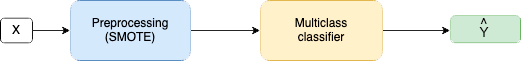
\includegraphics[scale=0.65]{multiclass-classifier}
			\caption{General model for the the three multiclass classification approaches.}
		\end{subfigure}
		\vskip\baselineskip
		% Start with figure tfrecord
		\begin{subfigure}[b]{\textwidth}
			\centering
			\captionsetup{justification=centering}
			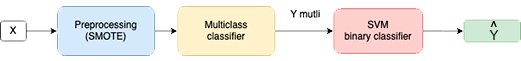
\includegraphics[scale=0.7]{mutli+svm-binary}
			\caption{Block diagram that shows the concatenation of multiclass classifier and the SVM binary classifier.}
		\end{subfigure}
		
		\caption{Confusion matrices for SVM multiclass classification for train and validation sets}
		\label{fig:mesh17}
	\end{figure}

	As previously explained in \ref{section:our-system}, as output of the multiclass systems, the soft values were obtained. These are the probabilities of a certain sample to belong to each class, being the highest value the one that usually corresponds to the correct predicted label. So this is exactly what we did: we took the highest probability and consider it the predicted category in order to transform the resulting outputs into hard format. This is the \textit{\^{Y}} in the figure. 
	
	For the binary approach, we just took the original soft outputs, \textit{Y multi}, to feed the binary classifier in order to be trained. The model for which the best accuracy value is obtained in the validation set was saved so as to, finally, use it in the testing process.
	
\subsection{Implementation 1: \acrshort{svm} classifier for a multiclass classification}
\label{subsection:implementation-1}

	We decided to establish a baseline by making a first experiment based on a \acrshort{svm} classifier that is used for a multiclass classification. In this case, we wanted to check the results of the performance of one of the most employed techniques in this filed different from \acrshort{nn}. It is true that this method is originally designed for binary problems but, as explained in \ref{subsection:svm}, we took advantage of the multiclass algorithm. To define our model, we used mainly the default parameters. In this work, we have not investigated which type of kernel could better fit our problem, however we found in the literature that the default option of \acrshort{rbf} is the most appropriated for real world applications \cite{Prajapati2010}. 
	
	Below, we can find the results for the different sets. In figure \ref{fig:mesh18}, the confusion matrices for the train and validation sets are shown. In figure \ref{fig:mesh19}, the confusion matrix for the evaluation on the test set is included. Finally, in the bar plot of figure \ref{fig:mesh20}, the accuracy values for the three sets are represented.
	
	\begin{figure}[ht]
		\hspace*{-2cm}
		% Whole figure
		\captionsetup{justification=centering}
		\begin{subfigure}[b]{\textwidth}
			% Start with figure wav
			\captionsetup{justification=centering}
			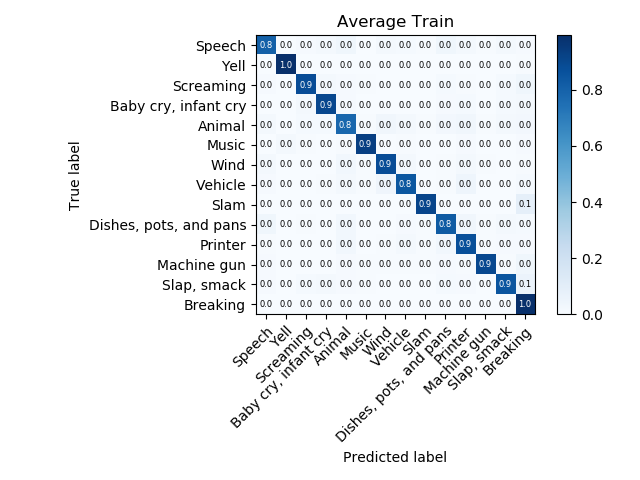
\includegraphics[width=0.6\linewidth]{svm-multi-cm-tr-av}%
			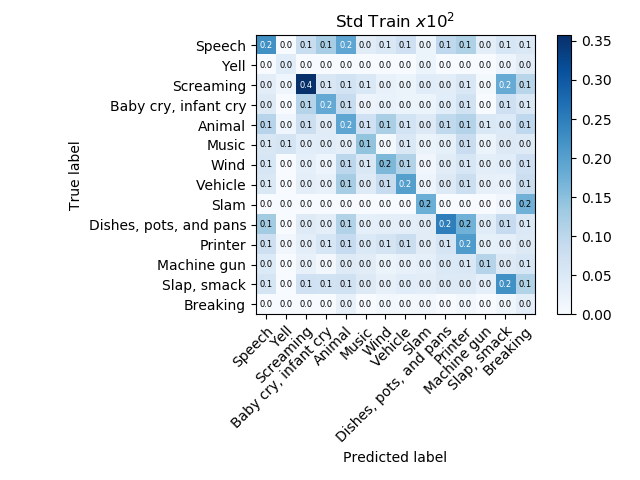
\includegraphics[width=0.6\linewidth]{svm-multi-cm-tr-std}
			\subcaption{Average and standard deviation for the train set}
		\end{subfigure}
		\vskip\baselineskip
		% Start with figure tfrecord
		\hspace*{-2cm}
		\begin{subfigure}[b]{\textwidth}
			\captionsetup{justification=centering}
			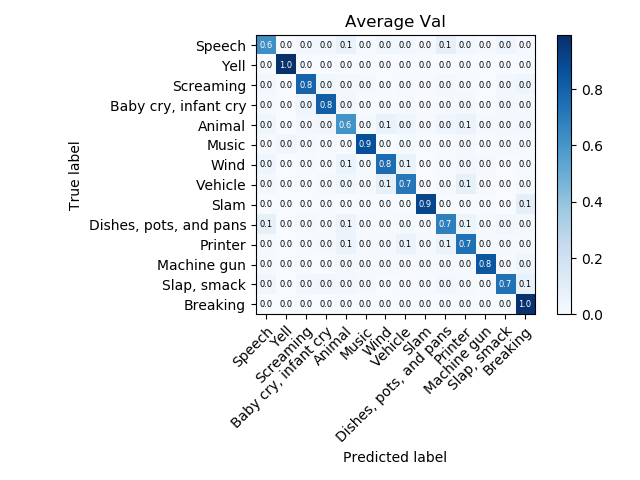
\includegraphics[width=0.6\linewidth]{svm-multi-cm-val-av}%
			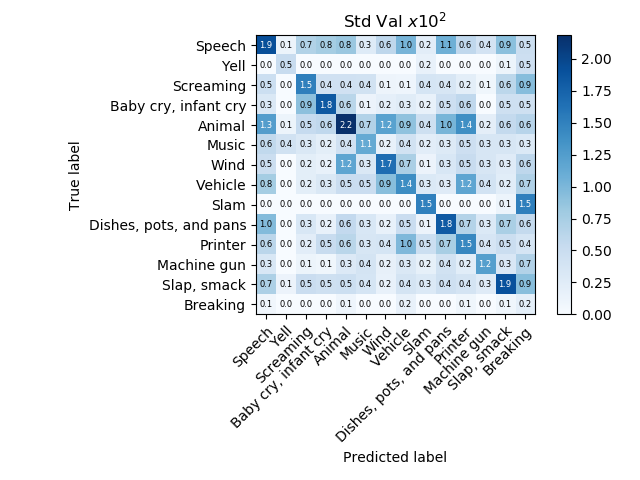
\includegraphics[width=0.6\linewidth]{svm-multi-cm-val-std}
			\subcaption{Average and standard deviation for the validation set}
		\end{subfigure}
		
		\caption{Confusion matrices for SVM multiclass classification for train and validation sets}
		\label{fig:mesh18}
	\end{figure}

	\begin{figure}[H]
		\centering
		\captionsetup{justification=centering}
		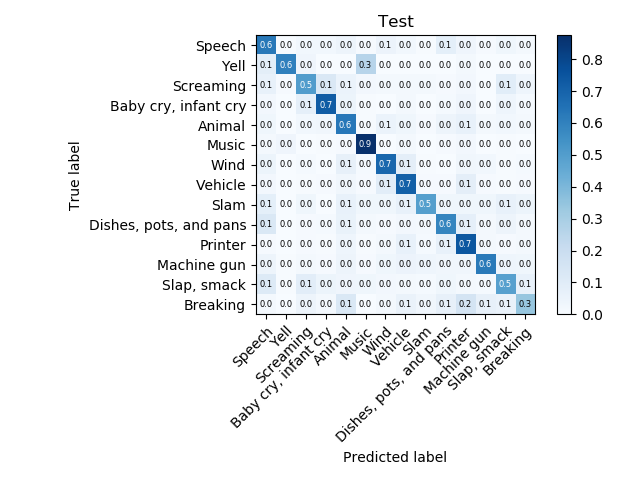
\includegraphics[width=0.6\linewidth]{svm-multi-cm-tst}
		\caption{Confusion matrix for the test set for the SVM multiclass classification}
		\label{fig:mesh19}
	\end{figure}

	\begin{figure}[H]
		\centering
		\captionsetup{justification=centering}
		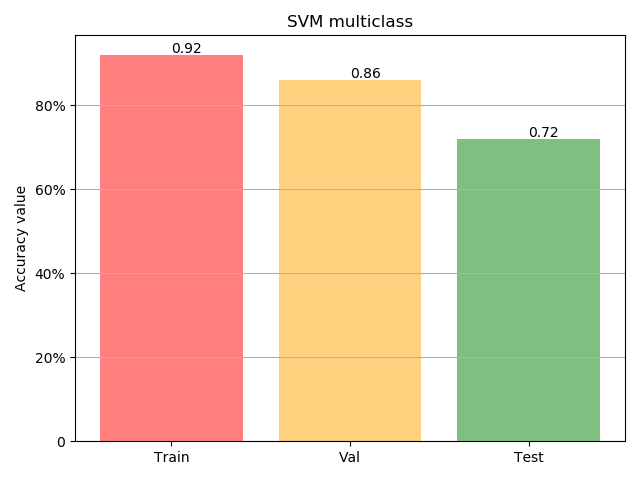
\includegraphics[width=0.55\linewidth]{svm-multierrorbar}
		\caption{Accuracy values for the three sets for the SVM multiclass classification}
		\label{fig:mesh20}
	\end{figure}

	The accuracy values are a $89\% \pm 0.087\%$ for the training set, a $79\% \pm 0.56\%$ for the validation and $69\%$ for test. This can also be appreciated in the average confusion matrices. The diagonal for the training and the validation stands out the other cells but they do not present a clear sense of overfitting due to they are not completely uniform. In the test results, we can see greater values in the true positive sections for the most populated classes, mentioned above in section \ref{section:input-data-preparation}. This makes sense since the test set has more samples in these categories. We can consider a good result for this case. The accuracy of the final testing process is not much lower than the one obtained for the validation set. It would be a good option to populate more the violent labels, but we did not want to use synthetic data in the final evaluation.
	
	In the table \ref{table:11}, a binary grouping considering the violent and non-violent classes is included. This was generated by taking the violent samples predicted as violence, even though the prediction did not match the specific class, it just had to be violent. Same for non-violent events. Also, the rest of the observations were grouped as predicted violent label for non-violent samples and vice versa.
	
	\begin{table}[H]
	\begin{center}
		\begin{tabular}{| m{6em} || m{6em} | m{6em} ||}
			\hline
			True/Predicted & \textbf{Non-violent} & \textbf{Violent} \\
			\hline\hline
			\textbf{Non-violent} & 5274 & 485 \\
			\hline
			\textbf{Violent} & 269 & 870 \\
			\hline
		\end{tabular}
	\end{center}
	\caption{Adaptation of the results for SVM multiclass classifier to binary}
	\label{table:11}
	\end{table}

	The accuracy value for this table is $89.07\%$, which was calculated by using the indicated formula in appendix \ref{appendix:metrics}. A grate difference is notable between the true positive section of the non-violent label with respect to the other parts of the matrix. However, we can considered an accurate result since plenty of the samples belong to true positive regions for all the classes in the confusion matrix for the test set in figure \ref{fig:mesh19}.

\subsection{Implementation 2: \acrshort{svm} multiclass classification and \acrshort{svm} binary classification}

	The \acrshort{svm} multiclass model is then incorporated to the previous stage of the preprocessing. So, it predicts the multiclass probability for each value, what can also be interpreted as it is converting the data to a new feature space before the binary classification.
	
	The results in accuracy and confusion matrices for the different evaluations can be found below. Figure \ref{fig:mesh23} includes the average and standard deviation of confusion matrices for train and validation sets. In figure \ref{fig:mesh24}, the confusion matrix for test is included. Then, in figure \ref{fig:mesh25}, the accuracy values for the three sets are shown.


	\begin{figure}[H]
		\hspace*{-2cm}
		\centering
		\captionsetup{justification=centering}
		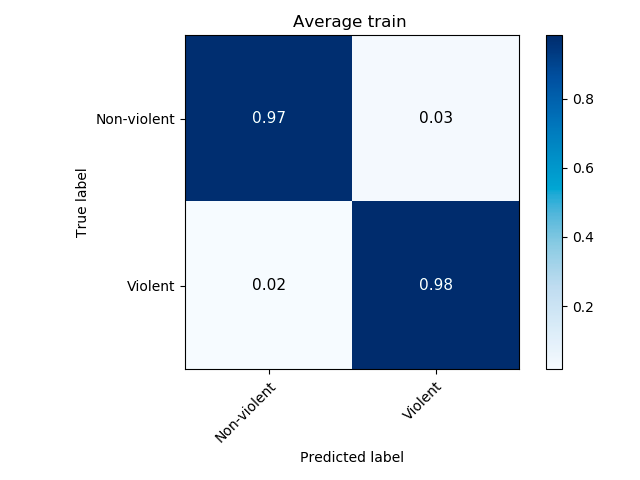
\includegraphics[width=0.6\linewidth]{svm-svm-cm-tr-av}%
		\includegraphics[width=0.6\linewidth]{svm-svm-cm-val-av}
		\caption{Confusion matrix for the train and validation sets for the SVM multiclass + SVM binary classification}
		\label{fig:mesh23}
	\end{figure}
	
	\begin{figure}[H]
		\centering
		\captionsetup{justification=centering}
		\includegraphics[width=0.6\linewidth]{svm-svm-cm-tst}
		\caption{Confusion matrix for the test set for the SVM multiclass + SVM binary classification}
		\label{fig:mesh24}
	\end{figure}

	In this performing model a more accurate interpretation can be obtained from paying attention to both metrics. In the accuracy bar plot, we can see that the values are $96\% \pm 0.024\%$ for the train set, a $96\% \pm 0.021\%$ for the validation set and a $90\%$ for the test. At first, it can be interpreted that the results are really good. This can be due to the high number of samples for a binary classification. Considering the test value of 90\%, we can see that the merit of the good performance is thank to the good classification of the non-violent observations, while the result on differentiating the violent classes is not as good since just the 67\% of the labels were correctly predicted. For the train and validation sets, the results are pretty good for both types, being a 96\% for both cases. Again, the fact of creating a big amount of the samples artificially for the training and validating parts is given a considerable difference in the results respect to the testing. However, this output also allows to see that with a more balanced test set the performance would be more even in the tree sets, as it happened with the multiclass task explained before, and that those observations which belong to the original embeddings show a satisfying outcome.

	\begin{figure}[H]
		\centering
		\captionsetup{justification=centering}
		\includegraphics[width=0.55\linewidth]{svm-binaryerrorbar}
		\caption{Accuracy values for the three sets for the SVM multiclass + SVM binary classification}
		\label{fig:mesh25}
	\end{figure}

	
\subsection{Implementation 3: \acrshort{lstm} for multiclass classification}

	\begin{wrapfigure}[12]{r}{0.35\textwidth}
		\centering
		\captionsetup{justification=centering}
		\includegraphics[width=0.5\linewidth]{lstm}
		\caption{LSTM architecture}
		\label{fig:mesh26}
	\end{wrapfigure}
	
	For this implementation we have decided to use a network composed by a total of three layers: two \acrshort{lstm} and a final \acrlong{fc} with a softmax activation function for the classification task. The first two \acrshort{lstm} layers are set with a drop-out of 0.05 and a recurrent dropout of 0.35. For the first one, the number of units was set to 128, in order not to change the dimensions of its output. In the second layer, it was set to 32 layers so as to reduce the dimensionality before the final prediction in the dense layer. In figure \ref{fig:mesh26}, an schema of the model is shown.
	
	The function minimized in the process was the categorical cross-entropy, which is a common way to evaluate multiclass classification problems. A more detailed explanation of this function can be found in appendix \ref{appendix:categorical-cross-entropy}. With respect to the training process, a number of 50 epochs were used and also a batch size of 32 samples. Also, a \acrshort{nadam} optimizer was used and a learning rate of $2e^{-3}$. An optimization algorithm is in charge of updating the internal parameters for a better performance and to minimize the loss function. The epochs is a hyperparameter that establishes how many times the learning algorithm pass through the entire train set in the training process. Finally, the batch size is the one that defines the number of observations the algorithm works through before assigns the internal parameters an updated value \cite{Browniee2018a}
	
	Below, the results for the classification are included. In figure \ref{fig:mesh27}, the average and standard deviation matrices for the train and validation sets are shown. Then, in figure \ref{fig:mesh28}, the confusion matrix for the testing process is included. In figure \ref{fig:mesh29}, a bar plot shows the accuracy for every set with their standard deviation values.
	
	\begin{figure}[H]
		% Whole figure
		\captionsetup{justification=centering}
		\hspace*{-3.5cm}
		\begin{subfigure}[b]{\textwidth}
			\centering
			\captionsetup{justification=centering}
			\includegraphics[width=0.6\linewidth]{lstm-multi-cm-tr-av}%
			\includegraphics[width=0.6\linewidth]{lstm-multi-cm-tr-std}
			\subcaption{Average and standard deviation for the train set}
		\end{subfigure}
		\vskip\baselineskip
		\hspace*{-3.5cm}
		\begin{subfigure}[b]{\textwidth}
			\centering
			\captionsetup{justification=centering}
			\includegraphics[width=0.6\linewidth]{lstm-multi-cm-val-av}%
			\includegraphics[width=0.6\linewidth]{lstm-multi-cm-val-std}
			\subcaption{Average and standard deviation for the validation set}
		\end{subfigure}
		\caption{Confusion matrices for LSTM multiclass classification for train and validation sets}
		\label{fig:mesh27}
	\end{figure}
	
	\begin{figure}[H]
		\centering
		\captionsetup{justification=centering}
		\includegraphics[width=0.6\linewidth]{lstm-multi-cm-tst}
		\caption{Confusion matrix for the test set for the LSTM multiclass classification}
		\label{fig:mesh28}
	\end{figure}
	
	\begin{figure}[H]
		\centering
		\captionsetup{justification=centering}
		\includegraphics[width=0.55\linewidth]{lstm-multierrorbar}
		\caption{Accuracy values for the three sets for the LSTM multiclass classification}
		\label{fig:mesh29}
	\end{figure}

	For this model, we obtained an accuracy of $79\% \pm 2.28\%$ for the training set, a $73\% \pm 2.41\%$ for the validation and a $61\%$ for the test. This can be due to the possible confusion regions mainly between classes such as \textit{Screaming} and \textit{Baby cry, infant cry}, and \textit{Wind} and \textit{Vehicle}, whose standard deviation values are the most emphasized. Also, a prominent failing region is the cell \textit{Slam}/\textit{Vehicle}, showing a not expected behaviour. About the \textit{Yell} class, there is a big misclassification that results in a majority of predicted \textit{Music} labels. The other violent classes have fewer correct predictions but also due to the fewer samples that belong to them in the test subset. We can discard heavy overfitting since the values of accuracy in the training and validation sets with respect to the test one are not too different. %away from each other.
	
	In table \ref{table:13}, the adaptation to the binary problem is included. The accuracy for this case is $88.27\%$. Of course, the true positive region with more samples is again the one that corresponds to non-violent. The observations placed in the false negative cell for the violent class can be a consequence of the misclassification of the samples form \textit{Yell} as \textit{Music}. Other cases of failed prediction as \textit{Breaking} for \textit{Slam} do not affect this matrix since the confusion occurs between violent classes.
	
	\begin{table}[H]
		\begin{center}
			\begin{tabular}{| m{6em} || m{6em} | m{6em} ||}
				\hline
				True/Predicted & \textbf{Non-violent} & \textbf{Violent} \\
				\hline\hline
				\textbf{Non-violent} & 517 & 62 \\
				\hline
				\textbf{Violent} & 20 & 100 \\
				\hline
			\end{tabular}
		\end{center}
		\caption{Adaptation of the results for LSTM multiclass classifier to binary}
		\label{table:13}
	\end{table}
	
	
\subsection{Implementation 4: \acrshort{lstm} multiclass + \acrshort{svm} for a final binary classification}
	
	For this case, the predicted probabilities obtained from the \acrshort{lstm} multiclass classifier are passed as input to the \acrshort{svm} for the binary classification. 
	
	The accuracy value for the different sets are included. Figure \ref{fig:mesh30} shows the average and standard deviation of the confusion matrices for the train and validation sets. In figure \ref{fig:mesh31}, the confusion matrix for the test set is also included, and in figure \ref{fig:mesh32}, the error bar can be seen with the accuracy values for each of the sets.
	
	\begin{figure}[H]
		\hspace*{-1.3cm}
		\centering
		\captionsetup{justification=centering}
		\includegraphics[width=0.55\linewidth]{lstm-svm-cm-tr-av}%
		\includegraphics[width=0.55\linewidth]{lstm-svm-cm-val-av}
		\caption{Average and standard deviation for the train and validation set for the LSTM multiclass + SVM binary classification}
		\label{fig:mesh30}
	\end{figure}

	\begin{figure}[H]
		\centering
		\captionsetup{justification=centering}
		\includegraphics[width=0.55\linewidth]{lstm-svm-cm-tst}
		\caption{Confusion matrix for the test set for the LSTM multiclass + SVM binary classification}
		\label{fig:mesh31}
	\end{figure}
	
	\begin{figure}[H]
		\centering
		\captionsetup{justification=centering}
		\includegraphics[width=0.55\linewidth]{lstm-svmerrorbar}
		\caption{Accuracy values for the three sets for the LSTM multiclass + SVM binary classification}
		\label{fig:mesh32}
	\end{figure}

	As shown in the bar plot, the values of the accuracy for train and validation are $94\% \pm 0.1\%$ and $94\% \pm 1\%$, respectively. The average matrices are really good as well. The no variation between them could be understood as a symptom of overfitting. However, the accuracy for testing is $90\%$, which is similar to the train and test results. The interesting point can be read in the confusion matrix for the test set. The classification of the violent classes is almost as good as the one for the non-violent ones, despite of the less amount of samples in these categories. 
	
\subsection{Implementation 5: \acrshort{cnn} for multiclass classification}

	For this case, we have implemented a \acrshort{cnn} model based on the architecture presented in figure \ref{fig:mesh5} in subsection \ref{subsection:exploring-differences-between-two-types-of-data-access} for the small experiment to check the similarity of the embeddings from the .\textit{tfrecord} files and the naturally audio files.
	
	In the configuration of the network, the same hyperparameters from implementation 3 are used for the learning process: a categorical cross-entropy for the loss function, a \acrshort{nadam} optimizer, a number of 50 epochs and a batch size of 32 samples. We have kept the same value for this model since the number of observations is the same and the depth of the network is not very great. A learning rate of $2e^{-3}$ was also used. 
	
	In figure \ref{fig:mesh33}, the average and standard deviation matrices for the train and validation sets are shown. In figure \ref{fig:mesh34}, the confusion matrix for the test set. The bar plot in \ref{fig:mesh35}, shows the accuracy for every set with their standard deviation values.
	
	\begin{figure}[H]
		\begin{center}
		% Whole figure
		\captionsetup{justification=centering}
		\begin{subfigure}[b]{\textwidth}
			% Start with figure wav
			\hspace*{-2cm}
			\centering
			\captionsetup{justification=centering}
			\includegraphics[width=0.6\linewidth]{cnn-multi-cm-tr-av}%
			\includegraphics[width=0.6\linewidth]{cnn-multi-cm-tr-std}
			\subcaption{Average and standard deviation for the train set}
		\end{subfigure}
		\vskip\baselineskip
		% Start with figure tfrecord
		\begin{subfigure}[b]{\textwidth}
			\hspace*{-2cm}
			\centering
			\captionsetup{justification=centering}
			\includegraphics[width=0.6\linewidth]{cnn-multi-cm-val-av}%
			\includegraphics[width=0.6\linewidth]{cnn-multi-cm-val-std}
			\subcaption{Average and standard deviation for the validation set}
		\end{subfigure}
		\caption{Confusion matrices for CNN multiclass classification for train and validation sets}
		\label{fig:mesh33}
		\end{center}
	\end{figure}
	
	\begin{figure}[H]
		\centering
		\captionsetup{justification=centering}
		\includegraphics[width=0.65\linewidth]{cnn-multi-cm-tst}
		\caption{Confusion matrix for the test set for the CNN multiclass classification}
		\label{fig:mesh34}
	\end{figure}
	
	\begin{figure}[H]
		\centering
		\captionsetup{justification=centering}
		\includegraphics[width=0.55\linewidth]{cnn-multierrorbar}
		\caption{Accuracy values for the three sets for the CNN multiclass classification}
		\label{fig:mesh35}
	\end{figure}

	The values of the accuracy obtained for this implementation are $98\% \pm 1\%$ for the train set, $72\% \pm 3\%$ for validation and $65\%$ for the test set. In the error bar in figure \ref{fig:mesh35}, the difference between the red bar for train is considerable meaningful with respect to the other two. Also, the confusion matrix for train shows a very well marked diagonal, while the other two are not that perfect. In the validation set, there are some misclassifications but still the equality among cells is present. Some confusion regions can be found again between \textit{Screaming} and \textit{Baby cry, infant cry} or \textit{Wind} and \textit{Vehicle}. In the test set, we can see that the diagonal does not follow a regular shape, being this one the worst result of the experiments.
	
	As in the previous cases, the table to see the problem from a binary point of view is included in \ref{table:13}. For this case the value of the accuracy is $90\%$. Again this result is kind of delicate. The failed predictions happen between, for example, \textit{Screaming} and \textit{Baby cry, infant cry}, and also between \textit{Breaking} and \textit{Slam}. Errors that this matrix does not show.
	
	\begin{table}[H]
	\begin{center}
		\begin{tabular}{| m{6em} || m{6em} | m{6em} ||}
		\hline
		True/Predicted & \textbf{Non-violent} & \textbf{Violent} \\
		\hline\hline
		\textbf{Non-violent} & 531 & 48 \\
		\hline
		\textbf{Violent} & 22 & 98 \\
		\hline
		\end{tabular}
	\end{center}
	\caption{Adaptation of the results for CNN multiclass classifier to binary}
	\label{table:12}
	\end{table}

\subsection{Implementation 6: \acrshort{cnn} multiclass + \acrshort{svm} for a final binary classification}

	In this last approach we wanted to use the predictions from the \acrshort{cnn} to feed the binary classifier \acrshort{svm}.
	
	Figure \ref{fig:mesh36} shows the average and standard deviation of the confusion matrices for the train and validation sets. Figure \ref{fig:mesh37} includes the confusion matrix for the test set. Finally, figure \ref{fig:mesh38} shows the error bar in which the accuracy values for the three test can be seen.
	
	\begin{figure}[H]
		\hspace*{-1.7cm}
		\centering
		\captionsetup{justification=centering}
		\includegraphics[width=0.6\linewidth]{cnn-svm-cm-tr-av}%
		\includegraphics[width=0.6\linewidth]{cnn-svm-cm-val-av}
		\caption{Average and standard deviation for the train and validation set for the CNN multiclass + SVM binary classification}
		\label{fig:mesh36}
	\end{figure}
	
	\begin{figure}[H]
		\centering
		\captionsetup{justification=centering}
		\includegraphics[width=0.6\linewidth]{cnn-svm-cm-tst}
		\caption{Confusion matrix for the test set for the CNN multiclass + SVM binary classification}
		\label{fig:mesh37}
	\end{figure}
	
	
	\begin{figure}[H]
		\centering
		\captionsetup{justification=centering}
		\includegraphics[width=0.55\linewidth]{cnn-svmerrorbar}
		\caption{Accuracy values for the three sets for the CNN multiclass + SVM binary classification}
		\label{fig:mesh38}
	\end{figure}

	The values of the accuracy are $98\% \pm 0.32\%$, $98\% \pm 3\%$ and $90\%$ for train, validation and test set, respectively. Again the results are similar to the ones obtained in the experiment 4. In this case, the classification of the violent classes are good enough as well for the test. However, as seen in experiment 5, there are plenty of misclassifications for the test set but some of them happen between classes of the same kind, so this failures do not have an effect on the binary problem. Also, others have been mixed with categories from the other group, this is would be the reason of the lower output. 
	
\section{Comparison and results}
	
	The idea behind the different implementations was to check the usefulness of the embeddings extracted with \acrshort{vgg}ish for a violent/non-violent classification problem. We wanted to study the performance of different learning techniques to see how this type of data worked with them. To do so, we first ran a typical algorithm for classification that does not involve \acrlong{nn}s, an \acrshort{svm}. Then, we thought it could be a good idea to try neural models with different core concepts to exploit the nature of our data. The dimensions of our input allowed the use of the \acrshort{cnn}, while the sequential character of an audio instance makes the \acrshort{lstm} a possible approach. In this section, we are going to compare the six different results dividing the explanations according to the type classification: multiclass or binary. 
	
	For the multiclass problem, the results are shown again in table \ref{table:9}.
	
	\begin{table}[h!]
		\begin{center}
			\resizebox{0.7\columnwidth}{!}{%
			\begin{tabular}{|| m{5em} | m{7em} | m{7em} | m{7em} ||}
				\hline
				& \textbf{Train} & \textbf{Validation} & \textbf{Test} \\
				\hline\hline
				\textbf{SVM} & $92\% \pm 0.087\%$ & $86\% \pm 0.56\%$ & $72\%$ \\
				\hline
				\textbf{\acrshort{lstm}} & $79\% \pm 2.28\%$ & $73\% \pm 2.41\%$ & $61\%$ \\
				\hline
				\textbf{\acrshort{cnn}} & $98\% \pm 1\%$ & $72\% \pm 3\%$ & $65\%$ \\
				\hline
			\end{tabular}
		}
		\end{center}
		\caption{Accuracy results for the three different algorithms and the three sets for the multiclass approach}
		\label{table:9}
	\end{table}

	Initially, the best performance for this case is the one done by with \acrshort{svm}. It is expectable that this algorithm achieves a good result due to the way it works. Basically, it expresses the different data samples in a feature space in which the optimal boundary is computed, as explained in subsection \ref{subsection:svm}. However, this one is not totally comparable with the other two \acrshort{lstm} and \acrshort{cnn}, since the number of observations to feed the model is much greater because of the conversions explained in the subsection \ref{section:input-data-preparation}. This way, the method has more examples to learn how the different classes are distributed.
	
	For the \acrshort{cnn} approach, the results are maybe the least satisfactory. The system presents a clear overfitting due to the big difference of the results for within the three sets. It is learning the data in the training stage and not being able to generalize, so it does not perform a good enough classification for validation and test. Also, considering the errors in figure \ref{fig:mesh34}, the mismatches are the greatest of the three experiments.
	
	In the \acrshort{lstm} approach, the results are numerically the worst but also the ones that make more sense. The system does not present an overfitting since the accuracies for validation and test are similar to the one for train. Also, most of the errors that can be read in the confusion matrix in figure \ref{fig:mesh31} are understandable since the audio data for those classes involved in the confusion regions may look similar. For example, a recording that belongs to \textit{Baby cry, infant cry} is likely to be similar to one from \textit{Screaming}. The same explanation could be used for \textit{Wind} and \textit{Vehicle}, since they usually have sounds that belong to scenes in a rush. Just some cases are more weird as the misclassification of \textit{Yell} for \textit{Music}, or \textit{Screaming} for \textit{Slap, smack}.
	
	Let's look at some violent categories to check their performance. 
	
	\begin{itemize}
		\item The error when predicting \textit{Music} for \textit{Yell} samples appears in all the models in a more or less clear way. Maybe, the original audio data from which the embeddings were extracted had common similarities. It would not be weird that many samples from \textit{Music} had the presence of shouts and yells.
		\item The confusion region between \textit{Screaming} and \textit{Baby cry, infant cry} comes out in all matrices. This makes sense, since the semantics of these two type of audio events is quite similar.
		\item The predictions for \textit{Slam} vary in all the models obtaining half of the samples correctly labeled for the \acrshort{svm} approach. In the case of the \acrshort{lstm} the true positive region just counts with $30\%$ of the data but the rest is misclassified among other violent categories. For the \acrshort{cnn}, this class is a complete failure being most of it classified as \textit{Speech}.
		\item In the case of \textit{Machine gun} it has a pretty good performance for all the three models, getting a $80\%$ for \acrshort{lstm}, a $70\%$ for \acrshort{cnn} and a $60\%$ in the case of \acrshort{svm} in the true positive regions. The rest of them are shared uniformly along all the other classes.
		\item In the case of \textit{Slap, smack}, it is predicted in a similar way for all the models as well, achieving a $50\%$ of the samples right classified.
		\item The class \textit{Breaking} has not showed a really good result for \acrshort{lstm} and \acrshort{cnn} being $40\%$ of the samples predicted as \textit{Slam}. However, for \acrshort{svm} a $30\%$ was set as true positives being the rest of the samples uniformly distributed along the other classes, mainly in \textit{Animal} and \textit{Printer}.
	\end{itemize}
	
   The conclusion we can extract from this comparison is that the models which shows much better results are the \acrshort{lstm} and \acrshort{svm}. We can see that the classes have similar results for all the methods being the \acrshort{svm} the one that stands out. In the \acrshort{lstm}, it calls the attention the region between \textit{Wind}, \textit{Vehicle} and \textit{Slam} and also the amount of samples from \textit{Yell} predicted as \textit{Music}. We could establish that maybe the \acrshort{cnn} is not the best option due to the broken diagonal that it presents. Also, a general good performance of the non-violent classes appears in all the matrices. This may be due to the more number of samples that belong to these classes within in the test set. It is worth to mention that the quality of the labels previously described in \ref{subsection:labels-quality}, can also affect the resulting values. For example, \textit{Yell} presents a quality of the $50\%$ and also \textit{Slam} has a label quality of $20\%$. This could be taken into account for future implementations.
   
   For the binary problem, the results are included in table \ref{table:10}. Also the confusion matrices for test are shown again in figure \ref{fig:mesh46}, since they are really relevant for the final explanation.
	
	\begin{table}[h!]
		\begin{center}
			\resizebox{0.7\columnwidth}{!}{%
			\begin{tabular}{|| m{5em} | m{7em} | m{7em} | m{7em} ||}
				\hline
				& \textbf{Train} & \textbf{Validation} & \textbf{Test} \\
				\hline\hline
				\textbf{SVM} & $96\% \pm 0.024\%$ & $96\% \pm 0.021\%$ & $90\%$ \\
				\hline
				\textbf{\acrshort{lstm}} & $ 94\% \pm 0.1\%$ & $95\% \pm 1\%$ & $90\%$ \\
				\hline
				\textbf{\acrshort{cnn}} & $98\% \pm 0.32\%$ & $98\% \pm 3\%$ & $90\%$ \\
				\hline
			\end{tabular}%
		}
		\end{center}
		\caption{Accuracy results for the three different algorithms and the three sets for the binary approach}
		\label{table:10}
	\end{table}
	
	\begin{figure}[H]
		\begin{center}
			% Whole figure
			\captionsetup{justification=centering}
			\begin{subfigure}[b]{\textwidth}
				\centering
				\captionsetup{justification=centering}
				\includegraphics[scale=0.45]{svm-svm-cm-tst}
				\subcaption{SVM multiclass + SVM binary}
			\end{subfigure}
			\vskip\baselineskip
			% 
			\begin{subfigure}[b]{\textwidth}
				\centering
				\captionsetup{justification=centering}
				\includegraphics[scale=0.45]{lstm-svm-cm-tst}
				\subcaption{LSTM multiclass + SVM binary}
			\end{subfigure}
			%
			\begin{subfigure}[b]{\textwidth}
				\centering
				\captionsetup{justification=centering}
				\includegraphics[scale=0.45]{cnn-svm-cm-tst}
				\subcaption{CNN multiclass + SVM binary}
			\end{subfigure}
			\caption{Test confusion matrices}
			\label{fig:mesh46}
		\end{center}
	\end{figure}

	The actual solution of the problem would be this binary classification that allows us to distinguish between non-violent and violent events. The results apparently are really good if we look at the accuracy values, but the interpretability is much more clear when reading the confusion matrices. 
	
	In order to interpret the result for the \acrshort{svm}, we can read the confusion matrix in figure \ref{fig:mesh19} to check how the multiclass classification performed and related to the output obtained from the binary classifier. For this case, certain classes have can be predicted within the range of false negatives as non-violent categories, such as \textit{Yell} confused with \textit{Music}. Also, a couple of categories are predicted as \textit{Speech} and some others as \textit{Animal}. If we interpret this errors in a binary context, we can say that the system is taking advantage of the higher a priory of non-violent classes without learning the true distinctions. %they can be resumed by saying that violent labels are predicted as non-violent. 
	This fact is reflected in the only $67\%$ of true positives for the violent label in figure \ref{fig:mesh46} \textit{(a)}. 
	
	In the \acrshort{cnn} approach, the results are numerically smaller but the classification of the violent instances is much better. Almost a $80\%$ of these samples were correctly classified. Again, if we look at figure \ref{fig:mesh34}, some classes are confused within the two different binary labels. A $30\%$ of instances from \textit{Slam} have been wrongly identified as \textit{Speech}. The same happens with \textit{Yell} and \textit{Music} as in the case of \acrshort{svm}. So, these can affect the output of this binary approach and the result of the test confusion matrix. There is also a big mistake in predicting \textit{Slam} for samples that belong to \textit{Breaking}, but this fact does not involve errors in the binary classification.
	
	Finally, the \acrshort{lstm} is the method for which a better result is obtained in this problem. In the confusion matrix in figure \ref{fig:mesh28}, as explained above, we can see some misclassifications but they happen between data of the same type, except between \textit{Yell} and \textit{Music}. In a real application this would be a more reasonable result, in order to detect a violent situation without depending too much on the exact event occurred just considering if it is violent or not. This is why the percentage of true positive samples for the violent class is the best for this model with a $86\%$. We can say that this is the best approach from all of our experiments. %the final experiment of the work is the one that involves \acrshort{lstm} as multiclass classifier.

		
	

\chapter{Conclusion}


\chapter{Future work}
% !TeX spellcheck = en_GB

	As explained in the section \ref{section:objectives}, this work can be defined as the very first approach of one of the parts of a much larger and ambitious project. So, it is easy to understand the future work is very extensive in order to fulfill the final requirements. However, we propose a couple of details and considerations that we thought a good idea when trying to implement our approach.
	
	One of the most important aspects when working on machine and deep learning problems is the quality and amount of data. Finding these resources is actually a really tough and long task. This is one of the first points that should be taken into account in order to go further in this investigation line. Researchers from the EMPATIA-TC project are currently working to solve this problem by trying to develop a database that collects data related to stimuli, labels for emotions and reactions of victims \cite{UC3M4SafetyTeam2018} in situations of violence against women. However, within the scope of this work, since the violence databases that are available do not focus on this task or are little populated, it would be interested to make a public dataset that allow to fully adapt the problem to the gender-based violence, including a wide range of sounds that may really happen in this kind of situations. This could be done in a much less complicated way without recording any victims, for example, by collecting audio data that strictly belong to this field from public websites and subject them to a proper labeling process.
	
	More work on trying to establish a subjective definition of violence that could be implemented is also possible. For our case, considering the way we chose, explained in subsection \ref{subsection:our-point-of-view}, a better implementation could be designed to ease the contribution of the victim to the whole learning process so it is not so annoying to be selecting all the categories, or, maybe, an automatic system in which the victim does not need to directly participate.
	
	Related to the feature extraction process, more studies could be done in order to finally select a feature space that totally adapts to the problem and makes the separability between violent and non-violent events available. If we consider the embeddings extracted with \acrshort{vgg}ish, a more immediate research line could be to try different values of the parameters related to the final shape of the embedding and overlapping between rows, as mentioned in subsection \ref{subsection:data-access}, so as to see the different results when extracting embeddings from audio data.
	
	 A good study to dive into is to improve the system used in the learning process by trying to apply new methods and algorithms or just taking more advantage of the ones already used, explained in subsection \ref{section:methodology} and chapter \ref{chapter:experiments}. For example, adapting the \acrshort{cnn} architecture model to the available data or improving the performance of the \acrshort{lstm}. In this last aspect, we did try to study a little the possibility of implementing an attention-based approach mixed with \acrshort{lstm}, following the idea proposed in \cite{Wang2016a} for sentiment analysis, but it was going to become very complex and out of our initial scope.
	 
	 Finally, the implementation of a model for multilabel\footnote{Multilabel classification differs from multiclass classification in the way the samples are labeled. The former treats samples that belong to more than one class at the same time, and the latter, the one implemented in this project, works with samples that belong to just one class.} classification. This is actually a very important topic that could increase the scope of the problem, also paying attention to its real world application. We just worked with single label samples from the dataset, which supposed a big limitation on the process of class selection. A bit of research was also done in order to make an attempt on this task by trying to use \acrfull{cc}, which treats the multilabel problem as a combination of several single label classifications \cite{Read2011}, but we did not get any further.
	 


%--------------
%	ACRÓNIMOS
%--------------
% \chapter*{Acronyms}
\printnoidxglossary[type=acronym]
%\printglossary[type=\acronymtype]
\printacronyms



%----------
%	BIBLIOGRAFÍA
%----------	

%\nocite{*} % Si quieres que aparezcan en la bibliografía todos los documentos que la componen (también los que no estén citados en el texto) descomenta está lína

\clearpage
\addcontentsline{toc}{chapter}{Bibliography}
\printbibliography



%----------
%	ANEXOS
%----------	

% Si tu trabajo incluye anexos, puedes descomentar las siguientes líneas
% Las páginas de los anexos no se numeran

\begin{appendix}
	% !TeX spellcheck = en_GB

\section{Metrics}
\label{appendix:metrics}

	A fundamental part of a machine learning project consists of checking the performance. There are plenty of metrics to carry out this evaluation and the results will look in one way or another depending on the method utilized. The following two are the most used in this project
	
\subsection{Classification Accuracy}

	This is a technique commonly used and it is usually referred to as just accuracy. It can be defined as the relation between the amount of right predictions and the total number on input instances \cite{Scikit-learn}.
	% Formula of accuracy
	\[
	\ \ acc = \frac{Number\ of\ incorrect\  predictions}{Number\ of\ total\ input\ instances}
	\]
	
	This metric best works when dealing with a balanced dataset, i.e., the same of number of samples per class.
	If the problem is addressed with unbalanced data, then the accuracy value could be a higher value due to predict all the instances belong to the major class. For example, if $90\%$ of the data are part of the same class A and all the predictions results are this class, then the accuracy value will be $90\%$, which apparently is a satisfying output, even though we are misclassifying all the samples from class B \cite{Mishra2018}. 
	
\subsection{Confusion matrix}

		% Confusion matrix exmaple
	\begin{figure}[b]
		\centering
		\captionsetup{justification=centering}
		\includegraphics[scale=0.6]{confusion-matrix}
		\caption{Example of confusion matrix}
		\label{fig:mesh6}
	\end{figure}

	As it own name describes, the output of this type of metric consists of a matrix which shows a complete evaluation of the model. By definition, an entry $i,j$ of the matrix denotes the amount of observations that belong to group $i$ but are predicted as group $j$ \cite{Scikit-learn}. For example, considering a binary classification problem in which there are two classes, YES and NO, for a test set composed by 165 samples, the matrix included in figure \ref{fig:mesh6} is obtained. 
	
	There are four groups that can be extracted from this matrix: True positives, the samples that are predicted as YES and that is in fact their true label, True Negatives, those cases that were predicted as NO and they are originally labelled as NO, False Positives, in which the predicted label is YES but they are actually negative, and False Negatives, those in which the predicted label is NO when their original label is YES.
	
	This metric an the one explained before, accuracy, can be related by taking the diagonal of the matrix and computing the next operation:
	
	\[
	\ \ acc = \frac{TruePositives +\ FalseNegatives}{Total\ number\ of\ samples} = 
	\ \ \frac{100 +\ 50}{165} = 0.91
	\]
	
	When the classification task consists on more than two classes, a multiclass problem, a similar definition of the confusion matrix can be extended from the binary problem. Considering a certain observation $C_k$, the True positive part of the matrix is placed in the exact point where the column and the row of this certain observation are crossed, i.e, when the predicted label is equal to the true label. The False positives samples are placed along the column $C_k$ for all the rows $C_0, ..., C_{k-1}, C{k+1}, ..., C_n$ which refers to all the samples that have been misclassified with the class $C_k$. The False negatives are, however, all the samples that originally are labelled with $C_k$ tag but have been wrongly categorized with $C_0, ..., C_{k-1}, C{k+1}, ..., C_n$ classes. Finally, the True negative samples are distributed across all the other positions in the matrix. In figure \ref{fig:mesh9}, a good example for this explanation is shown.
	
	\begin{figure}[h]
		\centering
		\captionsetup{justification=centering}
		\includegraphics[scale=0.4]{conf-mat-multi}
		\caption{Confusion matrix for a multiclass classification \cite{Kruger2018}}
		\label{fig:mesh9}
	\end{figure}
	
\section{\acrlong{kfold}}
\label{appendix:kfold}

	The cross-validation technique consists in a resampling practice that is commonly used in order to evaluate machine learning algorithms when the dataset is not very large. It just depends on the parameter $k$ which represents the amount of folds or groups the data is going to be split into. This is the reason of the k-fold prefix. When the method is referred to in a situation in which the parameter is already fixed, for example, if $k = 5$, it can becomes named as 5-fold cross-validation.
	
	The purpose of this procedure is to check the performance of a machine learning model on unseen data. This is for not evaluating with the data used for the training process. It is really used nowadays and allows to obtain a less biased estimation than if using other kind of techniques as just a simple train and test split \cite{Browniee2018}. The steps followed by the method are listed below \cite{M2018}.
	
	\begin{enumerate}
		\item The data is split in a random way into $k$ folds. The value of this parameter can be chosen previously by running the algorithm for different options and picking the one with the best performance. However, a not very high value is usually chosen, keeping it in a range between 5 and 10.
		\item Fit the model by using the data in the $k - 1$ folds as train set, and the other part in the $k$ fold for the validation process. Collect the results for this configuration.
		\item The process must be repeated until all folds have been used as the validation set. Then, the average and standard deviation of all the results can be computed as the metric of the model. 
	\end{enumerate}

	Sometimes, instead of dividing the whole set of data in $k$ folds, it is first done a split into train and test sets. Then, the test set is excluded for a final measure and the train is split again with the \acrlong{kfold} procedure. The concept of the technique is shown in figure \ref{fig:mesh16}.
	
	\begin{figure}[ht]
		\centering
		\captionsetup{justification=centering}
		\includegraphics[scale=0.35]{k-fold}
		\caption{K-fold cross-validation scheme. The data is first split into train and test, and then the train is split again with this method \cite{Scikit-learna}}
		\label{fig:mesh16}
	\end{figure}

	

\end{appendix}



\end{document}